\documentclass[11pt]{amsart}
\usepackage[margin=1.1in]{geometry}
\usepackage{amsmath,amssymb,amsthm,mathtools}
\usepackage{booktabs}
\usepackage{microtype}
\usepackage{xcolor}
\usepackage{tikz}
\usetikzlibrary{arrows.meta}
\usepackage[colorlinks=true,linkcolor=blue!50!black,citecolor=blue!50!black,urlcolor=blue!50!black]{hyperref}

\newtheorem{theorem}{Theorem}[section]
\newtheorem{proposition}[theorem]{Proposition}
\newtheorem{lemma}[theorem]{Lemma}
\newtheorem{corollary}[theorem]{Corollary}
\newtheorem{conjecture}[theorem]{Conjecture}
\theoremstyle{definition}
\newtheorem{definition}[theorem]{Definition}
\newtheorem{question}[theorem]{Question}
\theoremstyle{remark}
\newtheorem{remark}[theorem]{Remark}
\newtheorem{example}[theorem]{Example}

\newcommand{\Z}{\mathbb{Z}}
\newcommand{\F}{\mathbb{F}}
\newcommand{\A}{\mathcal{A}}
\newcommand{\Aut}{\operatorname{Aut}}
\newcommand{\End}{\operatorname{End}}
\newcommand{\Sym}{\operatorname{Sym}}
\newcommand{\Cent}{\mathcal{C}}
\newcommand{\sh}{\sigma}

\title[Fronts at the speed of light]{Fronts at the speed of light: rigidity of permutive second-order cellular automata}
\author{Michael Dayah}
\email{michael@dayah.com}
\date{November 5, 2026}

\subjclass[2020]{Primary 37B15; Secondary 37B10, 37B51, 20E08}
\keywords{Reversible cellular automata, second-order cellular automata, automorphism groups of subshifts, centralizers, spacetime subshifts, self-similar groups}

\begin{document}

\begin{abstract}
For an elementary rule $f$, the second-order (Fredkin) automaton $F_f$ on $(\{0,1\}^2)^{\Z}$ is reversible, and the automorphism group of its spacetime subshift $X_{F_f}$ is the centralizer of $F_f$ in the automorphism group of the full $4$-shift. It always contains $\langle\sh,F_f\rangle$, generated by the shift and the automaton. We prove that $\Aut(X_{F_f})=\langle\sh,F_f\rangle\cong\Z^2$ for rule $30$, for all $16$ elementary rules that are permutive in an outer variable and not affine (the classes of $30$, $45$, $75$ and $135$ under reflection and complementation), and for the $8$ rules in the classes of $63$ and $187$, which read only two neighbours and are not permutive. More generally, for a second-order automaton of any radius whose local rule is permutive in its leftmost variable, four conditions imply that the automorphism group is $\Z^2$: a stripping condition on the local rule, stronger than non-affineness for radius above $1$; the absence of a cellwise complement symmetry; strong connectivity of the light-speed window graphs, for which we give a sufficient finite certificate; and an index condition on spatially periodic orbits. The second condition is necessary. The proof follows the front at which a local difference spreads at the speed of light. A maximum principle shows that every automorphism shifts this front by a constant, and the same holds backwards in time; an automorphism with both offsets zero depends only on a light cone, and it must be the identity. For the rules that read two neighbours, the window graphs are identified with the action of a self-similar group on the $4$-ary tree, and the one-sided automorphisms are determined by induction on the anticipation.
\end{abstract}

\maketitle

\section{Introduction}\label{sec:intro}

Let $\A$ be a finite alphabet and $\sh$ the left shift on $\A^{\Z}$. By the Curtis--Hedlund--Lyndon theorem \cite{Hedlund1969} the endomorphisms of the full shift are the block maps, and its automorphisms are the invertible block maps. The group $\Aut(\A^{\Z})$ is very large: it contains every finite group and free groups \cite{BLR1988}, and every countable, locally finite, residually finite group \cite{KimRoush1990}, while its center consists of the powers of the shift \cite{Ryan1972}.

A reversible cellular automaton $F\in\Aut(\A^{\Z})$ determines a two-dimensional subshift, its \emph{spacetime} $X_F\subset\A^{\Z^2}$, whose rows are the configurations $F^n(c)$, $n\in\Z$; see Cyr, Franks and Kra \cite{CFK2019} for the spacetime of a general shift endomorphism. The automorphism group of $X_F$ is the centralizer of $F$ in $\Aut(\A^{\Z})$ (Lemma~\ref{lem:spacetime}), and it always contains the group $\langle\sh,F\rangle$. We ask when it contains nothing else. This is a case of the commuting block maps problem of Coven, Hedlund and Rhodes \cite{CHR1979}: to find all block maps that commute with a given one.

The automata we study are second-order automata, built by the second-order technique of Fredkin \cite{TM1990,Wolfram2002}; for radius $1$ they are the elementary reversible cellular automata introduced and studied systematically by Takesue \cite{Takesue1987,Takesue1989}. For a Boolean function $f$ of $2r+1$ variables, on the alphabet $\A=\{0,1\}^2$ with cells written $(x,y)$, put
\[
F_f(c)_i=\bigl(y_i,\;x_i\oplus f(y_{i-r},\dots,y_{i+r})\bigr).
\]
Reading $y$ as the current row and $x$ as the previous one, this is the recursion $y_{t+1}=y_{t-1}\oplus f(y_t)$, which is reversible for every $f$. For $r=1$ and $f$ an elementary rule, one writes $f$R for $F_f$, following Takesue \cite{Takesue1987}. A rule $f$ is \emph{permutive} in a variable if complementing that variable always changes the value of $f$ \cite{Hedlund1969}, and \emph{affine} if it is a sum modulo $2$ of some of its variables and a constant. Two rules are in the same \emph{class} if one is obtained from the other by reflecting the neighbourhood, by complementing all cells, or both; the corresponding automata are then conjugate (Section~\ref{pm:sec:classes}). For the elementary rules these are the $88$ classes of Takesue \cite{Takesue1987}, \cite[Table~I]{Takesue1989}.

Whether $\Aut(X_{F_f})$ is as small as $\langle\sh,F_f\rangle$ depends on $f$. For rule $54$ and many other elementary rules, words that $F_f$ fixes in every context act as walls, and permuting the contents of trains of identical segments between walls embeds every finite group in $\Aut(X_{F_f})$ \cite{PaperC}. In this paper we prove the opposite conclusion for two other families of rules: those that are permutive in an outer variable and not affine, and some that read only two neighbours.

\begin{theorem}[Theorem~\ref{thm:rigidity30}]\label{intro:thm:30}
$\Aut(X_{F_{30}})=\langle\sh,F_{30}\rangle$, and $(a,b)\mapsto\sh^aF_{30}^b$ is an isomorphism $\Z^2\to\langle\sh,F_{30}\rangle$.
\end{theorem}

\begin{theorem}[Theorem~\ref{pm:thm:main}]\label{intro:thm:pm}
Let $f$ be an elementary rule that is permutive in its left or its right variable and is not affine, that is, one of the sixteen rules
\[
30,\ 86,\ 106,\ 120,\qquad 45,\ 101,\ 166,\ 180,\qquad 75,\ 89,\ 154,\ 210,\qquad 135,\ 149,\ 169,\ 225.
\]
Then $\Aut(X_{F_f})=\langle\sh,F_f\rangle\cong\Z^2$.
\end{theorem}

\begin{theorem}[Theorem~\ref{hr:thm:main}]\label{intro:thm:hr}
Let $f$ be one of the eight rules $63$, $119$, $238$, $252$, $187$, $207$, $221$, $243$, which are not permutive in an outer variable and depend on only two of their three arguments. Then $\Aut(X_{F_f})=\langle\sh\rangle\times\langle F_f\rangle\cong\Z^2$.
\end{theorem}

In all three theorems there is no bound on the radius of the automorphisms, and the proofs are by hand; the finite checks they contain are set out in tables. The rules of Theorems~\ref{intro:thm:pm} and~\ref{intro:thm:hr} make up six of the $88$ classes of elementary rules; their place in the classification of all of them is discussed in \cite{PaperD}. In Takesue's study of these automata, $30$R and $75$R appear as rules with neither an additive conserved quantity on two adjacent cells nor a local conservation law on at most six cells \cite[Section~4 and Fig.~4]{Takesue1989}. Rule $110$, which is neither permutive nor of the form of Theorem~\ref{intro:thm:hr}, is treated by a different method in \cite{PaperA}.

The hypothesis that $f$ is not affine cannot be dropped. For the linear rule $150$, which is permutive in both outer variables, the map $\mathrm{id}+\sh F_{150}$ is an automorphism of $X_{F_{150}}$ outside $\langle\sh,F_{150}\rangle$ (Remark~\ref{pm:rem:linear}), and the automorphism group of the linear rule $90$ contains every finite group \cite{PaperC}. The proof shows where nonlinearity enters: only in one derivative identity, in the step that removes the correction term (fact (c) in the proof of Lemma~\ref{r30:lem:gamma}, and Lemma~\ref{gen:lem:steer} in general).

The method extends to any radius. Fix $r\ge1$ and a rule of the form $f(y_{i-r},\dots,y_{i+r})=y_{i-r}\oplus g(y_{i-r+1},\dots,y_{i+r})$, permutive in its leftmost variable, and let $F$ be the corresponding second-order automaton. Theorem~\ref{gen:main} uses four hypotheses (Definition~\ref{gen:def:hyp}): (N), that a second derivative $\partial_0\partial_jg$ is nonzero for some $j\ge r$, which for $r=1$ is non-affineness; (D), that $g$ is not self-dual, so that the cellwise complement $\kappa$ does not commute with $F$; ($\Lambda$), that the light-speed window graphs $\Lambda_M$ are strongly connected for every $M$; and (I), an index condition on the $\Z^2$-orbits of spatially periodic points.

\begin{theorem}[Theorems~\ref{gen:main} and~\ref{gen:structure}]\label{intro:thm:gen}
Under \textup{(N)}, \textup{(D)}, \textup{($\Lambda$)} and \textup{(I)}, $\Aut(X_F)=\langle\sh,F\rangle\cong\Z^2$. Under \textup{(N)}, \textup{(D)} and \textup{($\Lambda$)} alone, $\Aut(X_F)\cong\Z^2$, and $\langle\sh,F\rangle$ is a subgroup of index dividing $2r$ with cyclic quotient. If $g$ is self-dual, then $\kappa\in\Aut(X_F)\setminus\langle\sh,F\rangle$, so \textup{(D)} is necessary.
\end{theorem}

Hypothesis ($\Lambda$) follows from a finite certificate $(\mathrm T_P)$ on periodic histories that covers all $M$ at once (Proposition~\ref{gen:prop:TP}); the certificate is sufficient, and we do not know whether it is necessary. Hypothesis (I) is verified by enumerating spatially periodic points. For $r=1$ the four hypotheses hold for the eight left-permutive rules of Theorem~\ref{intro:thm:pm}, by hand, and this is how that theorem is proved (Section~\ref{sec:permutive}). The examples of larger radius are computer-assisted: for $r=2$, the certificate $(\mathrm T_P)$ with $P\le4$ holds for all $65\,504$ non-affine $g$, so that ($\Lambda$) holds for all of them (Proposition~\ref{gen:prop:r2TP}), and all four hypotheses hold for the thirteen rules of Proposition~\ref{gen:prop:r2}; for $r=3$ they hold for the six rules of Proposition~\ref{gen:prop:r3}. We conjecture that (N) can be weakened to non-affineness and that ($\Lambda$) holds for every non-affine $g$ (Conjectures~\ref{gen:conj:N} and~\ref{gen:conj:lambda}).

\subsection*{The method}
The known techniques for determining automorphism groups of $\Z^2$-subshifts do not apply to these spacetimes: the complexity arguments \cite{CK2015,DDMP2016} are for one-dimensional subshifts whose word complexity grows at most linearly or is not superlinear, while the rows of $X_F$ are arbitrary configurations; algebraic rigidity, which gives $\Aut=\Z^2$ for Ledrappier's shift \cite{Ledrappier1978} (\cite{Ward1994}, \cite[Theorem~7]{BRY2018}), needs a group shift; Hochman's theorem \cite{Hochman2010} needs positive $\Z^2$-entropy; and the finitary Ryan theorems \cite{Salo2019Ryan,Kopra2022} compute centralizers of sets of several automata. The closest results concern cellular automata that are permutive in both outer variables: their commutant is known to be small, and a bipermutive affine automaton commutes only with affine ones \cite{MooreBoykett1997,SaloTorma2013}. The automata $F_f$ are not permutive as automata on four letters (Remark~\ref{pm:rem:linear}), and these results give no description of the commutant of a nonlinear rule. The arguments below use specific properties of the rule.

What the proofs share with the low-complexity arguments is their object: an automorphism permutes the pairs of points that agree on a half-line (the right-asymptotic pairs), and it must respect the way in which their difference spreads. The lines along which it spreads, of slope $\pm1$ in spacetime, bound the light cone of \cite{CFK2019}; they play the role that nonexpansive directions play in the expansive subdynamics of Boyle and Lind \cite{BoyleLind1997}.

The property used for permutive rules is the light-speed front. Consider two configurations that agree far to the right. Because the rule is permutive in its left variable and the recursion is permutive in the previous row, the rightmost difference in their spacetime diagrams moves forward in time along a line of slope exactly $1$ and backward in time along a line of slope $-1$, with at most one exceptional row (Proposition~\ref{r30:prop:profile}). The main step (Theorem~\ref{r30:thm:front}) is that an automorphism shifts the forward line of every such pair by the same integer. The shift is a function of a finite window of the pair and is invariant under $F$. Its largest value is stable under arbitrary changes behind the front, by a maximum principle (Lemma~\ref{r30:lem:max}), so the set of words ahead of the front at which the maximum is attained is nonempty and forward-closed in the light-speed window graph $\Lambda_M$. When $\Lambda_M$ is strongly connected, it contains every word, and the shift is constant. The time reversal $\rho(x,y)=(y,x)$ gives the same for the backward line. This gives a homomorphism $\Aut(X_F)\to\Z^2$, injective on $\langle\sh,F\rangle$. An automorphism with both offsets zero depends only on a light cone (Proposition~\ref{r30:prop:cone}), is permutive in both edges of the cone (Proposition~\ref{r30:prop:edges}), and so is the identity plus a correction, which the commutation relation forces to vanish (Lemma~\ref{r30:lem:gamma}); nonlinearity enters only here. A parity argument on spatially periodic points (Lemma~\ref{r30:lem:parity}, and the index condition in general) shows that the image of the homomorphism is the image of $\langle\sh,F\rangle$.

Strong connectivity of $\Lambda_M$ is proved through a tower of factor graphs, in which each layer adds one bit and the lifting step needs a closed walk with odd holonomy. For rule $30$ this walk is a single loop (Lemma~\ref{r30:lem:lambda}); in general it comes from a time-periodic solution of the rule in comoving coordinates, supplied by the certificate $(\mathrm T_P)$.

For the rules that read two neighbours, the rightmost difference is invariant under $F$, and a maximum principle of the same kind shows that every automorphism moves it by a constant, once the window graphs are known to be strongly connected. Here they are identified with the action of a self-similar group on the $4$-ary tree, which is self-replicating and level-transitive (Proposition~\ref{hr:prop:tree}). An automorphism with offset zero reads only cells to its right, and an induction on the anticipation shows that the automorphisms with offset zero are exactly the powers of $F$ (Theorem~\ref{hr:thm:kernel}). In other words, $F$ defines an automorphism of the one-sided full shift on four letters \cite{BFK1990} whose centralizer there is $\langle F\rangle$ (Corollary~\ref{hr:cor:onesided}). The self-similar group is used in the language of \cite{Nekrashevych2005}.

\subsection*{Computations}
The proofs of Theorems~\ref{intro:thm:30}--\ref{intro:thm:hr} are by hand. Computations enter Theorem~\ref{intro:thm:gen} only through the certificates for the examples of radius $2$ and $3$, and every statement that depends on one is marked as computer-assisted. Computations also confirm the theorems independently: an exhaustive SAT enumeration of the block maps of radius at most $4$ commuting with $F_{30}$ gives only the maps $\sh^aF_{30}^b$ and two constant maps \cite{PaperD}, in agreement with Theorem~\ref{intro:thm:30}. Appendix~\ref{app:comp} specifies all computations, and the code accompanies the paper.

\subsection*{Organisation}
Section~\ref{sec:prelim} fixes notation and proves Lemma~\ref{lem:spacetime}. Section~\ref{sec:rigidity30} proves Theorem~\ref{intro:thm:30}; it is self-contained and is the model for the rest. Section~\ref{sec:general} treats permutive automata of any radius (Theorem~\ref{intro:thm:gen}), with examples, and Section~\ref{sec:permutive} derives Theorem~\ref{intro:thm:pm} from it. Section~\ref{sec:halfradius} proves Theorem~\ref{intro:thm:hr}; it does not depend on Sections~\ref{sec:general} and~\ref{sec:permutive}. Appendix~\ref{app:comp} describes the computations.

\emph{Both configurations of a pair.} The proofs in this paper follow one configuration along the front, through the graphs $\Lambda_M$. The supplement \cite{PaperBsupp} follows both configurations of a front pair, through a \emph{two-copy window graph} $\Gamma_{w,M}$: its vertices are the pairs of words that the two configurations of a front pair show on the $w$ cells behind the front, the front cell and the $M$ cells ahead of it, and its edges are the steps of $F$, one for each choice of the two cells that enter the window. For every left-permutive elementary rule, every walk of length $\lceil w/2\rceil$ in $\Gamma_{w,M}$ ends in a set of $2^{3w+2}4^M$ vertices that is closed under the edges; for the rules $30$, $45$, $75$ and $135$, and all $w\ge1$ and $M\ge0$, this set is strongly connected, so it is the unique terminal strongly connected component \cite[Theorem~3.1 and Proposition~8.2]{PaperBsupp}. None of this is used in the proofs of the theorems.

\section{Preliminaries}\label{sec:prelim}

Throughout, $\A=\{0,1\}^2$, and a cell $(x,y)\in\A$ is also written as the integer $2x+y\in\{0,1,2,3\}$; thus $3=(1,1)$ and $0=(0,0)$. The left shift is $\sh(c)_i=c_{i+1}$. A \emph{block map of radius $R$} is a map $h\colon\A^{\Z}\to\A^{\Z}$ of the form $h(c)_i=h_{\mathrm{loc}}(c_{i-R},\dots,c_{i+R})$ for a local rule $h_{\mathrm{loc}}\colon\A^{2R+1}\to\A$. A block map of radius $R$ is also a block map of every larger radius. By the Curtis--Hedlund--Lyndon theorem, $\End(\A^{\Z})$ is the monoid of block maps and $\Aut(\A^{\Z})$ the group of invertible ones. For a block map $F$ we write
\[
\Cent_R(F)=\{h\ \text{a block map of radius}\le R:\ h\circ F=F\circ h\},\qquad \Cent(F)=\bigcup_R\Cent_R(F),
\]
for the centralizer of $F$ in the monoid $\End(\A^{\Z})$; the centralizer of $F$ in the group $\Aut(\A^{\Z})$ is its group of invertible elements.

An elementary rule is a map $f\colon\{0,1\}^3\to\{0,1\}$, identified with its Wolfram number $\sum_{a,b,c}f(a,b,c)\,2^{4a+2b+c}$. Its second-order automaton $F_f$ is
\begin{equation}\label{eq:F}
F_f(c)_i=\bigl(y_i,\;x_i\oplus f(y_{i-1},y_i,y_{i+1})\bigr),
\end{equation}
where $c_i=(x_i,y_i)$. It is reversible, with inverse
\begin{equation}\label{eq:Finv}
F_f^{-1}(c)_i=\bigl(y_i\oplus f(x_{i-1},x_i,x_{i+1}),\,x_i\bigr).
\end{equation}
It has radius $1$, and $F_f^b$ has radius at most $|b|$, so $\sh^aF_f^b\in\Cent_{|a|+|b|}(F_f)$.

\begin{definition}
The \emph{spacetime subshift} of a reversible cellular automaton $F$ on $\A^{\Z}$ is
\[
X_F=\bigl\{(F^n(c))_{n\in\Z}:\ c\in\A^{\Z}\bigr\}\subset\A^{\Z^2},
\]
with the $\Z^2$-action generated by the horizontal shift $\sh$ and the vertical shift $\tau$, $(\tau z)_{n}=z_{n+1}$. An \emph{automorphism} of $X_F$ is a homeomorphism of $X_F$ commuting with both.
\end{definition}

\begin{lemma}\label{lem:spacetime}
For reversible $F$ the map $c\mapsto(F^n(c))_{n\in\Z}$ is a homeomorphism $\A^{\Z}\to X_F$ conjugating $(\sh,F)$ to $(\sh,\tau)$, and it induces an isomorphism
\[
\Aut(X_F)\;\cong\;\{h\in\Aut(\A^{\Z}):\ hF=Fh\}.
\]
Under this isomorphism $\langle\sh,\tau\rangle$ corresponds to $\langle\sh,F\rangle$.
\end{lemma}

\begin{proof}
The map is continuous, injective (the $0$-th row recovers $c$), and surjective onto $X_F$ by definition, hence a homeomorphism of compact spaces; it carries $\sh$ to $\sh$ and $F$ to $\tau$ since $F^{n}(F(c))=F^{n+1}(c)$. A homeomorphism of $\A^{\Z}$ commuting with $\sh$ is a block map by Curtis--Hedlund--Lyndon, and commuting with $\tau$ means commuting with $F$.
\end{proof}

So determining $\Aut(X_F)$ means determining the invertible block maps that commute with $F$, and $\Cent(F)$ is the monoid of endomorphisms of $X_F$. It contains non-invertible elements: the constant map onto a fixed point of $F$ is one. For every elementary rule with $f(0,0,0)=f(1,1,1)=0$, which includes $30$, both $(0,0)^{\Z}$ and $(1,1)^{\Z}$ are fixed by $F_f$, so $\Cent_R(F_f)$ contains these two constant maps for every $R$.


\section{Rule 30: the automorphism group is \texorpdfstring{$\Z^2$}{Z\^{}2}}\label{sec:rigidity30}

Throughout this section $f(a,b,c)=a\oplus(b\vee c)$ is rule $30$ and $F=F_{30}$, so that
\[
F(c)_i=\bigl(y_i,\;x_i\oplus y_{i-1}\oplus(y_i\vee y_{i+1})\bigr).
\]
By Lemma~\ref{lem:spacetime}, $\Aut(X_F)$ is the group of invertible block maps of $\A^{\Z}$ that commute with $F$, and we use this description throughout. We prove that for rule $30$ this group is as small as possible, namely $\langle\sh,F\rangle\cong\Z^2$.

\begin{theorem}\label{thm:rigidity30}
$\Aut(X_{F_{30}})=\langle\sh,F_{30}\rangle$, and $\langle\sh,F_{30}\rangle\cong\Z^2$. More precisely, every invertible block map $h$ with $hF_{30}=F_{30}h$ equals $\sh^aF_{30}^b$ for exactly one $(a,b)\in\Z^2$, namely $a=-\tfrac12(e^+(h)+e^-(h))$ and $b=\tfrac12(e^+(h)-e^-(h))$, where $e^+$ is the forward offset of Theorem~\ref{r30:thm:front}, which does not depend on the radius bound $R$ used to define it, and $e^-(h)=e^+(\rho h\rho)$ is the backward offset of Corollary~\ref{r30:cor:offsets}.
\end{theorem}

In particular $F_{30}$ has infinite order, and $\sh^aF_{30}^b=\mathrm{id}$ only for $a=b=0$; this part is elementary, since by Lemma~\ref{r30:lem:transl} the map $\sh^aF^b$ shifts the forward intercept of every pair by $b-a$ and the backward intercept by $-a-b$; applied to a single $y$-flip, whose intercepts are both finite, this shows that $\sh^aF^b$ moves them unless $a=b=0$. The theorem concerns automorphisms. The endomorphism monoid $\Cent(F_{30})$ contains the two constant maps onto the fixed points $(0,0)^{\Z}$ and $(1,1)^{\Z}$ (Section~\ref{sec:prelim}), and we do not determine it: the proof below uses the invertibility of $h$ in an essential way (Lemma~\ref{r30:lem:onset}).

\medskip
\noindent\textbf{Strategy.} We work with pairs of configurations that agree far to the right, and with the rightmost difference $\lambda_t$ in row $t$ of their spacetime diagrams. Because rule $30$ is permutive in its left argument and the second-order rule is permutive in the previous row, the rightmost difference moves forward in time along a line $i=t+U$ and backward in time along a line $i=V-t$, with at most one exceptional row between them (Proposition~\ref{r30:prop:profile}). We call $U$ and $V$ the forward and backward intercepts of the pair. The main step (Theorem~\ref{r30:thm:front}) is that an automorphism $h$ shifts the forward intercept of every \emph{front pair} (a pair whose rightmost difference is a $y$-bit) by the same integer $e^+(h)$. The shift $E(P)$ is a function of a finite window of the pair, and it is unchanged when the pair is advanced by $F$ (Lemma~\ref{r30:lem:E}). Let $e_{\max}$ be its largest value. A maximum principle (Lemma~\ref{r30:lem:max}) shows that the pairs with $E=e_{\max}$ stay so under arbitrary changes behind the front, so whether $E(P)=e_{\max}$ depends only on the cells of one configuration at and just ahead of the front (Corollary~\ref{r30:cor:word}). The set of words with this property is nonempty and forward-closed in a finite graph $\Lambda_M$ that follows one configuration along the light-speed front, and $\Lambda_M$ is strongly connected (Lemma~\ref{r30:lem:lambda}), so the set contains every word and the shift is constant. The graph $\Lambda_M$ is built as a tower of factor graphs in which each layer adds one bit, and the lifting step uses a closed walk along which the new bit changes an odd number of times; for rule $30$ this walk is a single loop. Constancy extends from front pairs to all pairs (Lemma~\ref{r30:lem:allpairs}), and through the time reversal $\rho(x,y)=(y,x)$ to the backward intercept. This gives a homomorphism $(e^+,e^-)\colon\Aut(X_F)\to\Z^2$ that is injective on $\langle\sh,F\rangle$. If $e^+(h)=e^-(h)=0$, then the value of $h$ at a point of spacetime depends only on the right light cone of that point (Proposition~\ref{r30:prop:cone}). It is permutive in both edges of the cone (Proposition~\ref{r30:prop:edges}), hence equals the identity plus a correction that depends only on the part of the cone strictly to the right of the apex, and the commutation relation forces the correction to vanish (Lemma~\ref{r30:lem:gamma}). Finally, a parity argument on the four spatially constant configurations shows that $e^+\equiv e^-\pmod 2$ (Lemma~\ref{r30:lem:parity}), so every automorphism is brought to offsets $(0,0)$ by an element of $\langle\sh,F\rangle$. Figure~\ref{r30:fig:profile} shows the profile of a pair, and Figure~\ref{r30:fig:cone} the light cone.

\medskip
\noindent\textbf{Conventions.} Bits are combined with $\oplus$, $\vee$, $\wedge$ and $\neg$. For a statement $S$, $[S]\in\{0,1\}$ is $1$ if $S$ holds and $0$ otherwise. Intervals $[m,n]$ are intervals of integers. We use $-\infty$ with the conventions $-\infty+k=-\infty<n$ for all integers $k,n$, and $\max\emptyset=-\infty$.

\subsection{Diagrams, pairs and profiles}\label{r30:sec:diagrams}

For $c\in\A^{\Z}$ and $t\in\Z$ let $y^t\in\{0,1\}^{\Z}$ be the $y$-row of $F^t(c)$. The $x$-row of $F(d)$ is the $y$-row of $d$, so the $x$-row of $F^t(c)$ is $y^{t-1}$, and in particular $c_i=(y^{-1}_i,y^0_i)$. The \emph{diagram} of $c$ is $Y_c\colon\Z^2\to\{0,1\}$, $Y_c(t,i)=y^t_i$. By \eqref{eq:F}, every diagram satisfies
\begin{equation}\label{r30:eq:rec}
Y(t+1,i)\oplus Y(t-1,i)\oplus Y(t,i-1)=Y(t,i)\vee Y(t,i+1)\qquad\text{for all }(t,i)\in\Z^2.
\end{equation}
The relation is an exclusive or in each of $Y(t+1,i)$, $Y(t-1,i)$ and $Y(t,i-1)$, so each of these three values is determined by the other four. Using the first two, any two consecutive rows determine all rows. Hence $c\mapsto Y_c$ is a bijection from $\A^{\Z}$ onto the set of solutions of \eqref{r30:eq:rec}, and two diagrams that agree on two consecutive rows are equal. Translations act by
\begin{equation}\label{r30:eq:transl}
Y_{\sh^jF^kc}(t,i)=Y_c(t+k,\,i+j).
\end{equation}
If $h$ is a block map commuting with $F$, then $F^th(c)=h(F^tc)$, so
\begin{equation}\label{r30:eq:rows}
\text{rows $t-1$ and $t$ of $Y_{hc}$ are the $x$-row and the $y$-row of $h(F^tc)$.}
\end{equation}

\paragraph{Time reversal.} Let $\rho\colon\A^{\Z}\to\A^{\Z}$ exchange the two bits of every cell, $\rho(c)_i=(y_i,x_i)$. That this exchange reverses time is noted in \cite[p.~2500]{Takesue1987}. From \eqref{eq:F}, $F(\rho c)_i=\bigl(x_i,\;y_i\oplus f(x_{i-1},x_i,x_{i+1})\bigr)$, so $\rho F\rho(c)_i=\bigl(y_i\oplus f(x_{i-1},x_i,x_{i+1}),\,x_i\bigr)=F^{-1}(c)_i$ by \eqref{eq:Finv}. Thus $\rho F\rho=F^{-1}$, and clearly $\rho\sh=\sh\rho$. Consequently $\rho h\rho$ is an invertible block map commuting with $F$ whenever $h$ is, and $h\mapsto\rho h\rho$ is an automorphism of the group $\Aut(X_F)$. Since $F^t\rho=\rho F^{-t}$ and the $y$-row of $\rho d$ is the $x$-row of $d$,
\begin{equation}\label{r30:eq:rho}
Y_{\rho c}(t,i)=Y_c(-1-t,\,i).
\end{equation}

\paragraph{Pairs and profiles.} A \emph{pair} is an ordered pair $Q=(c,c')$ of distinct configurations with $c_i=c'_i$ for all sufficiently large $i$. Its difference diagram is $\Delta_Q=Y_c\oplus Y_{c'}$. If $h$ is an invertible block map commuting with $F$, then $hQ=(hc,hc')$ is again a pair ($hc\ne hc'$ because $h$ is injective, and if $c,c'$ agree to the right of $s$ and $h$ has radius $R$, then $hc,hc'$ agree to the right of $s+R$), and so are $F^kQ$, $\sh^jQ$ and $\rho Q$, defined componentwise.

If rows $t-1$ and $t$ of $\Delta_Q$ vanish to the right of a site $s$, then by \eqref{r30:eq:rec} rows $t+1$ and $t-2$ vanish to the right of $s+1$. Rows $-1$ and $0$ vanish far to the right by definition, so by induction every row of $\Delta_Q$ does. The \emph{profile} of $Q$ is
\[
\lambda_t=\lambda_t(Q)=\max\{i:\Delta_Q(t,i)=1\}\in\Z\cup\{-\infty\}\qquad(t\in\Z).
\]

\begin{lemma}\label{r30:lem:R}
For every pair and every $t\in\Z$:
\begin{enumerate}
\item $\lambda_{t+1}\le\max(\lambda_{t-1},\lambda_t+1)$, with equality if $\lambda_{t-1}\ne\lambda_t+1$;
\item $\lambda_{t-1}\le\max(\lambda_{t+1},\lambda_t+1)$, with equality if $\lambda_{t+1}\ne\lambda_t+1$.
\end{enumerate}
\end{lemma}

\begin{proof}
By \eqref{r30:eq:rec},
\[
\Delta(t+1,i)=\Delta(t-1,i)\oplus\Delta(t,i-1)\oplus\bigl[(Y_c(t,i)\vee Y_c(t,i+1))\oplus(Y_{c'}(t,i)\vee Y_{c'}(t,i+1))\bigr].
\]
Let $m=\max(\lambda_{t-1},\lambda_t+1)$. For $i>m$ all three terms vanish, the last because $i,i+1>\lambda_t$. Suppose $m$ is finite. At $i=m$ the last term vanishes for the same reason. Since $m\ge\lambda_{t-1}$ and $m-1\ge\lambda_t$, we have $\Delta(t-1,m)=[m=\lambda_{t-1}]$ and $\Delta(t,m-1)=[m-1=\lambda_t]$. At least one of these is $1$, because $m$ is one of $\lambda_{t-1},\lambda_t+1$, and both are $1$ only if $\lambda_{t-1}=\lambda_t+1$. So $\Delta(t+1,m)=1$ when $\lambda_{t-1}\ne\lambda_t+1$. This proves (1). Part (2) is the same argument applied to \eqref{r30:eq:rec} solved for $Y(t-1,i)$, which has the same form with $t+1$ and $t-1$ exchanged.
\end{proof}

\begin{proposition}\label{r30:prop:profile}
Let $Q$ be a pair with profile $\lambda_t$, and put
\[
I^+=\{t:\lambda_t\ne-\infty,\ \lambda_t\ge\lambda_{t-1}\},\qquad I^-=\{t:\lambda_t\ne-\infty,\ \lambda_t\ge\lambda_{t+1}\}.
\]
\begin{enumerate}
\item No two consecutive $\lambda_t$ equal $-\infty$.
\item If $t\in I^+$, then $t+1\in I^+$ and $\lambda_{t+1}=\lambda_t+1$. If $t\in I^-$, then $t-1\in I^-$ and $\lambda_{t-1}=\lambda_t+1$. The sets $I^+$ and $I^-$ are disjoint, and every element of $I^-$ is smaller than every element of $I^+$.
\item The set $\Z\setminus(I^+\cup I^-)$ has at most one element. If $m$ is such an element (a \emph{middle row}), then $m-1\in I^-$, $m+1\in I^+$ and $\lambda_m<\lambda_{m-1}=\lambda_{m+1}$. If $I^+=\emptyset$ then $I^-=\Z$, and if $I^-=\emptyset$ then $I^+=\Z$.
\item Define the \emph{forward intercept} $U=U(Q)$ and the \emph{backward intercept} $V=V(Q)$ by $U=\lambda_t-t$ for $t\in I^+$ and $V=\lambda_t+t$ for $t\in I^-$ (well defined by (2)), with $U=-\infty$ if $I^+=\emptyset$ and $V=-\infty$ if $I^-=\emptyset$. Then $\lambda_t\le\max(t+U,\,V-t)$ for all $t$. Equivalently, $\Delta_Q(t,i)=1$ implies $i-t\le U$ or $i+t\le V$.
\item Suppose $U$ and $V$ are finite. If $V-U$ is odd, there is no middle row, and $I^+=[t_+,\infty)$, $I^-=(-\infty,t_+-1]$ with $2t_+-1=V-U$. If $V-U$ is even, there is a middle row $m=(V-U)/2$, and $I^+=[m+1,\infty)$, $I^-=(-\infty,m-1]$.
\item For every $t$, $U\le\max(\lambda_t-t,\ \lambda_{t-1}-t-1)$ and $V\le\max(\lambda_t+t,\ \lambda_{t+1}+t-1)$.
\end{enumerate}
\end{proposition}

\begin{figure}[ht]
\centering
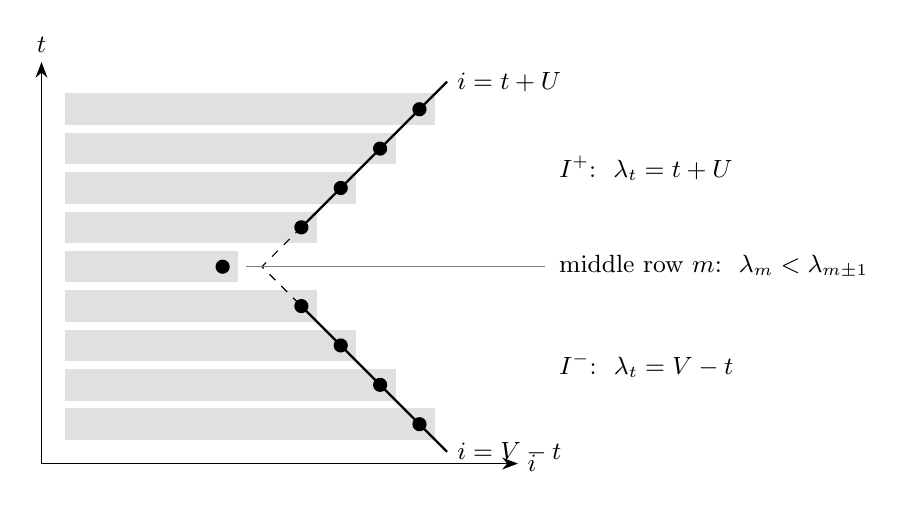
\begin{tikzpicture}[x=0.5cm,y=0.5cm,font=\small]
\foreach \t/\l in {-2/6,-1/5,0/4,1/3,2/1,3/3,4/4,5/5,6/6}{
  \fill[black!12] (-3,\t-0.4) rectangle (\l+0.4,\t+0.4);
  \fill (\l,\t) circle (0.18);
}
\draw[thick] (3,3) -- (6.7,6.7) node[right] {$i=t+U$};
\draw[thick] (3,1) -- (6.7,-2.7) node[right] {$i=V-t$};
\draw[dashed] (3,3) -- (2,2) -- (3,1);
\draw[-{Stealth[length=2mm]}] (-3.6,-3) -- (-3.6,7.2) node[above] {$t$};
\draw[-{Stealth[length=2mm]}] (-3.6,-3) -- (8.5,-3) node[right] {$i$};
\node[right] at (9.3,4.5) {$I^+$:\ \ $\lambda_t=t+U$};
\node[right] at (9.3,2) {middle row $m$:\ \ $\lambda_m<\lambda_{m\pm1}$};
\node[right] at (9.3,-0.5) {$I^-$:\ \ $\lambda_t=V-t$};
\draw[black!50] (9.2,2) -- (1.6,2);
\end{tikzpicture}
\caption{The profile of a pair with $U$, $V$ finite and $V-U$ even (Proposition~\ref{r30:prop:profile}). Each row $t$ of the difference diagram vanishes outside the shaded sites $i\le\lambda_t$, and the dot marks the rightmost difference $\lambda_t$. It moves along the line $i=t+U$ for $t\in I^+$ and along $i=V-t$ for $t\in I^-$; the two lines meet in the middle row $m=(V-U)/2$. If $V-U$ is odd there is no middle row.}
\label{r30:fig:profile}
\end{figure}

\begin{proof}
(1) If $\lambda_t=\lambda_{t+1}=-\infty$, then $Y_c$ and $Y_{c'}$ agree on two consecutive rows, so $c=c'$, which is excluded.

(2) If $t\in I^+$ then $\lambda_{t-1}\le\lambda_t<\lambda_t+1$, so Lemma~\ref{r30:lem:R}(1) gives $\lambda_{t+1}=\max(\lambda_{t-1},\lambda_t+1)=\lambda_t+1$; in particular $\lambda_{t+1}\ge\lambda_t$, so $t+1\in I^+$. The statement for $I^-$ follows in the same way from Lemma~\ref{r30:lem:R}(2). If $t\in I^+$ then $\lambda_{t+1}>\lambda_t$, so $t\notin I^-$. If $a\in I^+$ and $b\in I^-$ with $a\le b$, then $b\in I^+$ by the first statement, contradicting disjointness.

(3) Let $t\notin I^+\cup I^-$. If $\lambda_t=-\infty$, then $\lambda_{t\pm1}$ are finite by (1), and $\lambda_{t+1}\ge\lambda_t$, $\lambda_{t-1}\ge\lambda_t$ give $t+1\in I^+$, $t-1\in I^-$. If $\lambda_t$ is finite, then $t\notin I^+$ gives $\lambda_{t-1}>\lambda_t$ (in particular $\lambda_{t-1}$ is finite), so $t-1\in I^-$; and $t\notin I^-$ gives $\lambda_{t+1}>\lambda_t$, so $t+1\in I^+$. If $t<t'$ were two such elements, then $t+1\in I^+$ and (2) would give $t'\in I^+$. Hence there is at most one. If $I^+=\emptyset$, no such element can exist (it would have $t+1\in I^+$), so $I^-=\Z$; symmetrically for $I^-=\emptyset$.

Now let $m$ be a middle row; we have shown $m\pm1\in I^\pm$ and $\lambda_m<\lambda_{m\pm1}$. If $\lambda_m=-\infty$, then $\lambda_{m-1}\ne\lambda_m+1$ and Lemma~\ref{r30:lem:R}(1) gives $\lambda_{m+1}=\lambda_{m-1}$. If $\lambda_m$ is finite and $\lambda_{m-1}\ne\lambda_m+1$, then Lemma~\ref{r30:lem:R}(1) gives $\lambda_{m+1}=\max(\lambda_{m-1},\lambda_m+1)=\lambda_{m-1}$, since $\lambda_{m-1}\ge\lambda_m+1$. If $\lambda_{m-1}=\lambda_m+1$, then $\lambda_{m+1}\le\lambda_m+1$ by Lemma~\ref{r30:lem:R}(1), and $\lambda_{m+1}>\lambda_m$, so $\lambda_{m+1}=\lambda_m+1=\lambda_{m-1}$.

(4) For $t\in I^+$ we have $\lambda_t=t+U$ and for $t\in I^-$ we have $\lambda_t=V-t$. For a middle row $m$, $\lambda_m<\lambda_{m-1}=V-m+1$, so $\lambda_m\le V-m$.

(5) Both $I^+$ and $I^-$ are nonempty. By (2) and (3), $\Z$ is the disjoint union of an interval $I^-=(-\infty,t_-]$, at most one middle row, and an interval $I^+=[t_+,\infty)$. If there is no middle row, then $t_-=t_+-1$; now $t_+\in I^+$ gives $t_++U\ge\lambda_{t_+-1}=V-t_++1$, and $t_+-1\in I^-$ gives $V-t_++1\ge t_++U$, so $V-U=2t_+-1$. If there is a middle row $m$, then $\lambda_{m+1}=\lambda_{m-1}$ reads $m+1+U=V-m+1$, so $V-U=2m$. The two cases give different parities of $V-U$, so the parity decides which case occurs.

(6) Put $\mu_t=\max(\lambda_t-t,\ \lambda_{t-1}-t-1)$. By Lemma~\ref{r30:lem:R}(1), $\lambda_{t+1}-(t+1)\le\max(\lambda_{t-1}-t-1,\ \lambda_t-t)\le\mu_t$, and $\lambda_t-t-2<\lambda_t-t\le\mu_t$, so $\mu_{t+1}\le\mu_t$. If $I^+\ne\emptyset$, then for $t-1\in I^+$ we have $\mu_t=\max(U,U-2)=U$. As $\mu$ is nonincreasing, $U\le\mu_t$ for every $t$; if $I^+=\emptyset$ there is nothing to prove. Similarly $\nu_t=\max(\lambda_t+t,\ \lambda_{t+1}+t-1)$ is nondecreasing by Lemma~\ref{r30:lem:R}(2), and $\nu_t=V$ whenever $t+1\in I^-$; hence $V\le\nu_t$ for every $t$.
\end{proof}

\begin{lemma}\label{r30:lem:transl}
For every pair $Q$ and all $j,k\in\Z$:
$U(F^kQ)=U(Q)+k$ and $V(F^kQ)=V(Q)-k$;
$U(\sh^jQ)=U(Q)-j$ and $V(\sh^jQ)=V(Q)-j$;
$U(\rho Q)=V(Q)+1$ and $V(\rho Q)=U(Q)-1$.
\end{lemma}

\begin{proof}
By \eqref{r30:eq:transl}, $\lambda_t(F^kQ)=\lambda_{t+k}(Q)$ and $\lambda_t(\sh^jQ)=\lambda_t(Q)-j$. So $I^\pm(F^kQ)=I^\pm(Q)-k$, $I^\pm(\sh^jQ)=I^\pm(Q)$, and the formulas for $F^k$ and $\sh^j$ follow. By \eqref{r30:eq:rho}, $\lambda_t(\rho Q)=\lambda_{-1-t}(Q)$. Hence $t\in I^+(\rho Q)$ if and only if $-1-t\in I^-(Q)$, and then $\lambda_t(\rho Q)=V(Q)-(-1-t)=t+V(Q)+1$; and $t\in I^-(\rho Q)$ if and only if $-1-t\in I^+(Q)$, and then $\lambda_t(\rho Q)=(-1-t)+U(Q)=U(Q)-1-t$. The values $-\infty$ correspond to empty sets on both sides.
\end{proof}

\begin{definition}\label{r30:def:front}
A pair $(c,c')$ is a \emph{front pair at $p$} if $c_i=c'_i$ for all $i>p$, $y(c_p)\ne y(c'_p)$ and $x(c_p)=x(c'_p)$; equivalently, $\lambda_0=p>\lambda_{-1}$. For $c\in\A^{\Z}$ and $j\in\Z$, the \emph{$y$-flip}, \emph{$x$-flip} and \emph{$yx$-flip at $j$} are the pairs $(c,c')$ in which $c'$ is obtained from $c$ by complementing, respectively, the bit $y(c_j)$; the bit $x(c_j)$; both bits $y(c_j)$ and $x(c_{j+1})$.
\end{definition}

\begin{lemma}\label{r30:lem:flips}
\begin{enumerate}
\item If $Q$ is a front pair at $p$, then $U(Q)=p$, and $F^tQ$ is a front pair at $p+t$ for every $t\ge0$.
\item A $y$-flip at $j$ is a front pair at $j$, with $(U,V)=(j,j-2)$.
\item If $Q$ is an $x$-flip at $j$, then $FQ$ is a front pair at $j$, and $(U,V)=(j-1,j-1)$.
\item A $yx$-flip at $j$ has $V=j$, and either $U=-\infty$ or $U\le j-1$.
\end{enumerate}
\end{lemma}

\begin{proof}
(1) Here $0\in I^+$, so $U=\lambda_0=p$, and by Proposition~\ref{r30:prop:profile}(2), $\lambda_t=p+t>\lambda_{t-1}$ for all $t\ge0$. Since $\lambda_0(F^tQ)=\lambda_t$ and $\lambda_{-1}(F^tQ)=\lambda_{t-1}$, this says that $F^tQ$ is a front pair at $p+t$.

(2) Here $\lambda_0=j$ and $\lambda_{-1}=-\infty$, so the pair is a front pair at $j$ and $U=j$ by (1). By Lemma~\ref{r30:lem:R}(2) at $t=-1$, since $\lambda_0\ne\lambda_{-1}+1$, $\lambda_{-2}=\max(\lambda_0,\lambda_{-1}+1)=j$. Thus $-2\in I^-$ and $V=j-2$.

(3) Here $\lambda_{-1}=j$ and $\lambda_0=-\infty$. By Lemma~\ref{r30:lem:R}(1) at $t=0$, $\lambda_1=\max(j,-\infty)=j$. So $\lambda_0(FQ)=j>\lambda_{-1}(FQ)=-\infty$, $FQ$ is a front pair at $j$, $1\in I^+$ and $U=j-1$. Also $-1\in I^-$ because $\lambda_{-1}\ge\lambda_0$, so $V=j-1$.

(4) Here $\lambda_0=j$ and $\lambda_{-1}=j+1$, so $-1\in I^-$ and $V=j$. By Lemma~\ref{r30:lem:R}(1), $\lambda_1\le j+1$, and by \eqref{r30:eq:rec}, $\Delta(1,j+1)=\Delta(-1,j+1)\oplus\Delta(0,j)\oplus0=1\oplus1=0$, the last term vanishing because row $0$ of $\Delta$ vanishes at $j+1$ and $j+2$. So $\lambda_1\le j$, and Proposition~\ref{r30:prop:profile}(6) at $t=1$ gives $U\le\max(\lambda_1-1,\lambda_0-2)\le j-1$.
\end{proof}

\subsection{The light-speed window graph}\label{r30:sec:window}

Fix $M\ge0$. Let $\Lambda_M$ be the directed graph whose vertices are the words $\omega=\omega_0\cdots\omega_M\in\A^{M+1}$, with an edge $\omega\to\omega\cdot\iota$ for every $\iota=(\iota_1,\iota_2)\in\A^2$, where
\[
(\omega\cdot\iota)_k=F(\tilde c)_{p+1+k}\qquad(0\le k\le M)
\]
and $\tilde c$ is any configuration with $\tilde c_{p+k}=\omega_k$ for $0\le k\le M$, $\tilde c_{p+M+1}=\iota_1$ and $\tilde c_{p+M+2}=\iota_2$. Since $F$ has radius $1$, the cells $F(\tilde c)_i$ with $p+1\le i\le p+M+1$ read only $\tilde c$ on $[p,p+M+2]$, so $\omega\cdot\iota$ depends neither on $p$ nor on the other cells of $\tilde c$. A vertex of $\Lambda_M$ is the word of a single configuration on a cell $p$ (the \emph{front}) and the $M$ cells ahead of it, and an edge advances the front by one site, at the speed of light.

\begin{lemma}\label{r30:lem:lambda}
For every $M\ge0$, the graph $\Lambda_M$ is strongly connected.
\end{lemma}

The proof occupies the rest of this subsection. It builds $\Lambda_M$ as a tower of $2M+2$ factor graphs, each of which adds one bit to the previous one (Figure~\ref{r30:fig:layers}).

\paragraph{Layer coordinates.} For a vertex $\omega$ of $\Lambda_M$, placed on the sites $[p,p+M]$, put
\begin{equation}\label{r30:eq:layers}
y[d]=y(\omega_{-d})\ \ (-M\le d\le0),\qquad x[k]=x(\omega_{-k-1})\ \ (-M-1\le k\le-1).
\end{equation}
Thus the cell at site $p-d$ is $(x[d-1],y[d])$, and a vertex is the same as an arbitrary assignment of bits to the $2M+2$ \emph{layers} $y[-M],\dots,y[0]$ and $x[-M-1],\dots,x[-1]$. The index of a layer is a comoving coordinate: if $c$ is a configuration and $z_t[d]$ denotes the $y$-bit of $F^t(c)$ at site $p+t-d$, then the word of $F^t(c)$ on $[p+t,p+t+M]$ has $y$-layers $z_t[d]$ and $x$-layers $z_{t-1}[k]$.

\begin{figure}[ht]
\centering
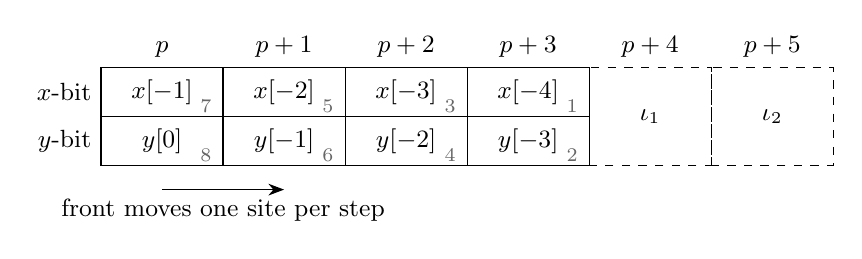
\begin{tikzpicture}[x=1.55cm,y=0.62cm,font=\small]
\foreach \j/\d in {0/0,1/-1,2/-2,3/-3}{
  \draw (\j,0) rectangle (\j+1,1);
  \draw (\j,1) rectangle (\j+1,2);
}
\node at (0.5,1.5) {$x[-1]$}; \node at (0.5,0.5) {$y[0]$};
\node at (1.5,1.5) {$x[-2]$}; \node at (1.5,0.5) {$y[-1]$};
\node at (2.5,1.5) {$x[-3]$}; \node at (2.5,0.5) {$y[-2]$};
\node at (3.5,1.5) {$x[-4]$}; \node at (3.5,0.5) {$y[-3]$};
\node[above] at (0.5,2) {$p$}; \node[above] at (1.5,2) {$p+1$}; \node[above] at (2.5,2) {$p+2$}; \node[above] at (3.5,2) {$p+3$};
\node[left] at (0,1.5) {$x$-bit}; \node[left] at (0,0.5) {$y$-bit};
\foreach \j/\a/\b in {0/7/8,1/5/6,2/3/4,3/1/2}{
  \node[font=\scriptsize,text=black!60] at (\j+0.86,1.2) {\a};
  \node[font=\scriptsize,text=black!60] at (\j+0.86,0.2) {\b};
}
\draw[dashed] (4,0) rectangle (5,2); \draw[dashed] (5,0) rectangle (6,2);
\node at (4.5,1) {$\iota_1$}; \node at (5.5,1) {$\iota_2$};
\node[above] at (4.5,2) {$p+4$}; \node[above] at (5.5,2) {$p+5$};
\draw[-{Stealth[length=2mm]}] (0.5,-0.5) -- node[below] {front moves one site per step} (1.5,-0.5);
\end{tikzpicture}
\caption{A vertex of $\Lambda_M$ for $M=3$, with its layer coordinates \eqref{r30:eq:layers} and the two input cells $\iota_1,\iota_2$ of an edge. The small numbers give the order $L_1,\dots,L_8$ in which the tower adds the layers: from the cell farthest ahead of the front back to the front, and within a cell first the $x$-bit, then the $y$-bit.}
\label{r30:fig:layers}
\end{figure}

\begin{lemma}[layer equation]\label{r30:lem:layer}
Let $\omega$ be a vertex of $\Lambda_M$ and $\iota=(\iota_1,\iota_2)\in\A^2$, let $y',x'$ be the layers of $\omega'=\omega\cdot\iota$, and put
\[
u=y(\iota_1),\qquad v=x(\iota_1)\oplus y(\omega_M)\oplus\bigl(y(\iota_1)\vee y(\iota_2)\bigr).
\]
Then:
\begin{enumerate}
\item $x'[-M-1]=u$, and $x'[k]=y[k]$ for $-M\le k\le-1$;
\item $y'[-M]=v$;
\item for $-M+1\le d\le0$,
\begin{equation}\label{r30:eq:L}
y'[d]=y[d]\oplus x[d-2]\oplus\bigl(y[d-1]\vee y[d-2]\bigr),
\end{equation}
with the convention $y[-M-1]=u$.
\end{enumerate}
The map $\iota\mapsto(u,v)$ is onto $\{0,1\}^2$. So every vertex $\omega$ has exactly four successors, the vertices $\omega\cdot(u,v)$, $(u,v)\in\{0,1\}^2$, given by \textup{(1)--(3)}.
\end{lemma}

\begin{proof}
Let $\tilde c$ be as in the definition of $\omega\cdot\iota$. The new cell at a site $i$ is $F(\tilde c)_i=\bigl(y(\tilde c_i),\,x(\tilde c_i)\oplus y(\tilde c_{i-1})\oplus(y(\tilde c_i)\vee y(\tilde c_{i+1}))\bigr)$, and the layers of $\omega'$ are taken with respect to the new front $p+1$. So $x'[k]$ is the $x$-bit of the new cell at site $p-k$, which is the old $y$-bit at that site: this is $y[k]$ if $p-k\le p+M$, and $y(\iota_1)=u$ if $k=-M-1$. Likewise $y'[d]$ is the $y$-bit of the new cell at site $i=p+1-d$. For $d=-M$ this site is $p+M+1$, and the bit is $v$. For $d\ge-M+1$ we have $i\le p+M$, and $x(\tilde c_i)=x[d-2]$, $y(\tilde c_{i-1})=y[d]$, $y(\tilde c_i)=y[d-1]$ and $y(\tilde c_{i+1})=y[d-2]$, where $y[-M-1]$ stands for the $y$-bit at site $p+M+1$, which is $u$. Given $(u,v)$, take $y(\iota_1)=u$, any $\iota_2$, and $x(\iota_1)=v\oplus y(\omega_M)\oplus(u\vee y(\iota_2))$.
\end{proof}

Equation \eqref{r30:eq:L} is \eqref{r30:eq:rec} written in comoving coordinates. It is lower triangular: $y'[d]$ reads only layers with index at most $d$.

\paragraph{The tower.} Order the $N=2M+2$ layers as
\[
L_1=x[-M-1],\ \ L_2=y[-M],\ \ L_3=x[-M],\ \ L_4=y[-M+1],\ \ \dots,\ \ L_{N-1}=x[-1],\ \ L_N=y[0],
\]
that is, $x[d-1]$ followed by $y[d]$ for $d=-M,\dots,0$. Let $P_n=\{L_1,\dots,L_n\}$, and let $\pi_n$ be the restriction of an assignment of bits to $P_n$. By Lemma~\ref{r30:lem:layer}, the new value of each layer depends only on $(u,v)$ and on layers that precede it or equal it in this order: $x'[k]$ is $u$ or $y[k]$, which precedes $x[k]$; $y'[-M]$ is $v$; and $y'[d]$ reads $y[d]$ and the earlier layers $x[d-2]$, $y[d-1]$ and $y[d-2]$ (or $u$). Hence $\pi_n(\omega\cdot(u,v))$ depends only on $\pi_n(\omega)$ and $(u,v)$. Let $\Lambda^{(n)}$ be the graph with vertex set $\{0,1\}^{P_n}$ and an edge $\eta\to\eta\cdot(u,v):=\pi_n(\omega\cdot(u,v))$, labelled $(u,v)$, for every $\eta$ and $(u,v)$, where $\omega$ is any vertex of $\Lambda_M$ with $\pi_n(\omega)=\eta$. Then:
\begin{itemize}
\item $\Lambda^{(N)}$ has the same vertices and the same successor sets as $\Lambda_M$, so one is strongly connected if and only if the other is;
\item every walk of $\Lambda^{(n)}$ lifts, with the same labels, to a walk of $\Lambda^{(n+1)}$ starting at any vertex that restricts to its initial vertex.
\end{itemize}

\begin{proof}[Proof of Lemma~\ref{r30:lem:lambda}]
We show by induction on $n$ that $\Lambda^{(n)}$ is strongly connected for $2\le n\le N$.

\emph{Base.} The vertices of $\Lambda^{(2)}$ are the values of $(x[-M-1],y[-M])$, and by Lemma~\ref{r30:lem:layer}(1),(2) the edge labelled $(u,v)$ leads from every vertex to $(u,v)$. So $\Lambda^{(2)}$ is a complete digraph with loops.

\emph{Predecessors.} Every vertex $\omega_2$ of $\Lambda_M$, with layers $y_2,x_2$, has an in-neighbour, and every in-neighbour $\hat\omega$ of $\omega_2$, with layers $\hat y,\hat x$, satisfies $\hat y[k]=x_2[k]$ for $-M\le k\le-1$. The second statement is Lemma~\ref{r30:lem:layer}(1). For the first, put $u=x_2[-M-1]$, $v=y_2[-M]$, $\hat y[k]=x_2[k]$ for $-M\le k\le-1$ and $\hat y[0]=0$, and then, with $\hat y[-M-1]=u$,
\[
\hat x[d-2]=y_2[d]\oplus\hat y[d]\oplus\bigl(\hat y[d-1]\vee\hat y[d-2]\bigr)\qquad(-M+1\le d\le0),
\]
and $\hat x[-1]=0$. The indices $d-2$ are distinct and lie in $[-M-1,-2]$, so this defines a vertex $\hat\omega$, and $\hat\omega\cdot(u,v)=\omega_2$ by Lemma~\ref{r30:lem:layer}.

\emph{The step $L_{n+1}=x[k]$, $-M\le k\le-1$.} Assume $\Lambda^{(n)}$ is strongly connected. Write the vertices of $\Lambda^{(n+1)}$ as $(\eta,\chi)$ with $\eta\in\{0,1\}^{P_n}$ and $\chi$ the bit $x[k]$. By Lemma~\ref{r30:lem:layer}, the layer $x[k]$ is read, if at all, only by $y'[k+2]$, which is not in $P_{n+1}$, and its new value is $x'[k]=y[k]$, with $y[k]\in P_n$. So the edge labelled $(u,v)$ goes from $(\eta,\chi)$ to $(\eta\cdot(u,v),\,y[k](\eta))$. Let $(\eta_1,\chi_1)$ and $(\eta_2,\chi_2)$ be vertices of $\Lambda^{(n+1)}$. Extend $(\eta_2,\chi_2)$ to a vertex $\omega_2$ of $\Lambda_M$ and take an in-neighbour $\hat\omega$ of $\omega_2$, with $\hat\omega\cdot(u,v)=\omega_2$. Then $\hat\eta=\pi_n(\hat\omega)$ has an edge labelled $(u,v)$ to $\eta_2$, and $y[k](\hat\eta)=\hat y[k]=x_2[k]=\chi_2$. Take a walk from $\eta_1$ to $\hat\eta$ in $\Lambda^{(n)}$ and lift it to $\Lambda^{(n+1)}$ starting at $(\eta_1,\chi_1)$. It ends at $(\hat\eta,\chi')$ for some $\chi'$, and the edge labelled $(u,v)$ then leads to $(\eta_2,\chi_2)$.

\emph{The step $L_{n+1}=y[d]$, $-M+1\le d\le0$.} Assume $\Lambda^{(n)}$ is strongly connected. Here $P_n$ consists of all layers with index at most $d-1$. For an edge of $\Lambda^{(n)}$ from $\eta$ with label $(u,v)$ put
\[
\phi=x[d-2]\oplus\bigl(y[d-1]\vee y[d-2]\bigr)\in\Z/2,
\]
evaluated on $\eta$, with $y[-M-1]=u$. By \eqref{r30:eq:L}, the edges of $\Lambda^{(n+1)}$ are $(\eta,z)\to(\eta\cdot(u,v),\,z\oplus\phi)$, where $z$ is the bit $y[d]$. The \emph{holonomy} of a walk of $\Lambda^{(n)}$ is the sum in $\Z/2$ of $\phi$ over its edges; the lift of the walk from $(\eta,z)$ ends at a vertex whose last bit is $z$ plus the holonomy.

Let $\eta_*\in\{0,1\}^{P_n}$ be the vertex with
\begin{equation}\label{r30:eq:loop}
y[d-1]=x[d-1]=1,\qquad\text{and all other layers of $P_n$ equal to $0$.}
\end{equation}
We claim that the edge from $\eta_*$ labelled $(u,v)=(0,\,y[-M])$ is a loop, with $\phi=1$. Indeed, by Lemma~\ref{r30:lem:layer}(1), $x'[-M-1]=u=0$ and $x'[k]=y[k]=x[k]$ for $-M\le k\le d-1$, and by (2), $y'[-M]=v=y[-M]$. For $-M+1\le i\le d-1$ the layers $y[i-1]$, $y[i-2]$ and $x[i-2]$ have index at most $d-2$, so they vanish (for $i-2=-M-1$, by $u=0$), and \eqref{r30:eq:L} gives $y'[i]=y[i]$. Finally $\phi=x[d-2]\oplus(y[d-1]\vee y[d-2])=0\oplus(1\vee y[d-2])=1$.

So $\Lambda^{(n)}$ has a closed walk with holonomy $1$, namely this loop. Let $\eta_2$ be any vertex of $\Lambda^{(n)}$, and choose walks $\alpha$ from $\eta_2$ to $\eta_*$ and $\beta$ from $\eta_*$ to $\eta_2$. The closed walks at $\eta_2$ formed by $\alpha$ followed by $\beta$, and by $\alpha$, the loop and $\beta$, have holonomies of different parity. So there are closed walks of both parities at every vertex. Given vertices $(\eta_1,z_1)$ and $(\eta_2,z_2)$ of $\Lambda^{(n+1)}$, take a walk from $\eta_1$ to $\eta_2$ in $\Lambda^{(n)}$ followed by a closed walk at $\eta_2$, chosen so that the total holonomy is $z_1\oplus z_2$. Its lift from $(\eta_1,z_1)$ ends at $(\eta_2,z_2)$.

Every layer $L_{n+1}$ with $n\ge2$ is covered by one of the two steps, so $\Lambda^{(N)}$ is strongly connected, and hence so is $\Lambda_M$.
\end{proof}

The form $a\oplus(b\vee c)$ of rule $30$ enters this proof only through the loop at $\eta_*$: it is a stationary solution of \eqref{r30:eq:L} on the layers below $d$ that cannot be continued to the layer $y[d]$. For other rules the loop is replaced by closed walks that come from time-periodic solutions (Section~\ref{gen:sec:tower}).

\subsection{The front offset}\label{r30:sec:front}

In this subsection $h$ is an invertible block map commuting with $F$, and $R\ge1$ is an integer bounding the radii of both $h$ and $h^{-1}$. Lemmas~\ref{r30:lem:onset}, \ref{r30:lem:E} and~\ref{r30:lem:max} and Corollary~\ref{r30:cor:word} use nothing about the rule beyond Lemma~\ref{r30:lem:R} and its consequences in Section~\ref{r30:sec:diagrams}; the rule enters the proof of Theorem~\ref{r30:thm:front} only through Lemma~\ref{r30:lem:lambda}.

\begin{lemma}\label{r30:lem:onset}
Let $P$ be a front pair at $p$. Then $U(hP)$ is finite, $|U(hP)-p|\le R$, and $I^+(hP)\supseteq[R+1,\infty)$; that is, $\lambda_t(hP)=t+U(hP)$ for every $t\ge R+1$.
\end{lemma}

\begin{proof}
Write $\lambda_t=\lambda_t(hP)$, $P=(c,c')$, and let $t\ge0$. By Lemma~\ref{r30:lem:flips}(1), $F^tP$ is a front pair at $p+t$, and by \eqref{r30:eq:rows}, rows $t-1$ and $t$ of $\Delta_{hP}$ record where $h(F^tc)$ and $h(F^tc')$ differ in the $x$-bit and in the $y$-bit. Since $h$ has radius at most $R$, these images agree at every site $i>p+t+R$, so $\lambda_t,\lambda_{t-1}\le p+t+R$. Since $h^{-1}$ has radius at most $R$ and $F^tc$, $F^tc'$ differ at site $p+t$, the images differ at some site in $[p+t-R,\,p+t+R]$, so $\max(\lambda_t,\lambda_{t-1})\ge p+t-R$.

Let $t_+=\min I^+$, with $t_+=\infty$ if $I^+=\emptyset$. Suppose $t_+\ge2$. By Proposition~\ref{r30:prop:profile}(2),(3), every $t\le t_+-2$ lies in $I^-$ (in particular $I^-\ne\emptyset$ and $V=V(hP)$ is finite), and the row $t_+-1$ lies in $I^-$ or is the middle row. In both cases $\lambda_t\le V-t$ for all $t\le t_+-1$, by Proposition~\ref{r30:prop:profile}(4) (if $t_+=\infty$, then $I^-=\Z$). As $-1\in I^-$, the upper bound at $t=0$ gives $V+1=\lambda_{-1}\le p+R$. For $1\le t\le t_+-1$ we get
\[
p+t-R\le\max(\lambda_t,\lambda_{t-1})\le V-t+1\le p+R-t,
\]
so $t\le R$. If $t_+=\infty$ this fails at $t=R+1$, a contradiction; otherwise taking $t=t_+-1$ gives $t_+\le R+1$. So in all cases $t_+\le R+1$, and $U$ is finite. For $t\ge R+1$ we have $t\in I^+$, so $\lambda_t=t+U\ge\lambda_{t-1}$, and the two bounds give $p+t-R\le t+U\le p+t+R$.
\end{proof}

For a front pair $P$ at $p$ put
\[
E(P)=U(hP)-p.
\]
This quantity is intrinsic: it does not involve $R$.

\begin{lemma}\label{r30:lem:E}
Let $P=(c,c')$ be a front pair at $p$.
\begin{enumerate}
\item $E(P)\in[-R,R]$, and $E(P)$ depends only on the restrictions of $c$ and $c'$ to $[p-2R,\,p+4R+2]$: if $\tilde P=(\tilde c,\tilde c')$ is a front pair at $p$ with $\tilde c=c$ and $\tilde c'=c'$ on this interval, then $E(\tilde P)=E(P)$.
\item $E(\sh^jP)=E(P)$ for every $j\in\Z$.
\item $E(FP)=E(P)$.
\item $(c',c)$ is a front pair at $p$, and $E(c',c)=E(c,c')$.
\end{enumerate}
\end{lemma}

\begin{proof}
(1) $E(P)\in[-R,R]$ is Lemma~\ref{r30:lem:onset}. By that lemma, $R+1\in I^+(hP)$, so $U(hP)=\lambda_{R+1}(hP)-R-1$. By \eqref{r30:eq:rows}, $\lambda_{R+1}(hP)$ is the largest site at which the $y$-bits of $h(F^{R+1}c)$ and $h(F^{R+1}c')$ differ. Since $F^{R+1}P$ is a front pair at $p+R+1$, these images agree at all sites beyond $p+2R+1$, and $\lambda_{R+1}(hP)=U(hP)+R+1\ge p+1$. So $\lambda_{R+1}(hP)$ is the largest site $i\in[p+1,\,p+2R+1]$ at which the $y$-bits of $h(F^{R+1}c)_i$ and $h(F^{R+1}c')_i$ differ. These bits depend only on $F^{R+1}c$ and $F^{R+1}c'$ on $[p+1-R,\,p+3R+1]$, hence only on $c$ and $c'$ on $[p-2R,\,p+4R+2]$. The same description applies to $\tilde P$, and since $\tilde P$ agrees with $P$ on this interval, the same bits are compared. So $\lambda_{R+1}(h\tilde P)=\lambda_{R+1}(hP)$ and $E(\tilde P)=E(P)$.
(2) $\sh^jP$ is a front pair at $p-j$, and $U(h\sh^jP)=U(\sh^jhP)=U(hP)-j$ by Lemma~\ref{r30:lem:transl}.
(3) $FP$ is a front pair at $p+1$ by Lemma~\ref{r30:lem:flips}(1). Since $hF=Fh$, Lemma~\ref{r30:lem:transl} gives $U(hFP)=U(FhP)=U(hP)+1$.
(4) The conditions of Definition~\ref{r30:def:front} are symmetric in $c$ and $c'$. The difference diagram $\Delta_{h(c',c)}=Y_{hc'}\oplus Y_{hc}$ equals $\Delta_{h(c,c')}$, and $U$ is a function of the difference diagram.
\end{proof}

Front pairs exist, and $E$ takes values in the finite set $[-R,R]$, so
\[
e_{\max}=\max\{E(P):P\text{ a front pair at some }p\in\Z\}
\]
exists.

\begin{lemma}[maximum principle]\label{r30:lem:max}
Let $P=(c,c')$ be a front pair at $p$ with $E(P)=e_{\max}$.
\begin{enumerate}
\item If $c''$ agrees with $c'$ at every site $i\ge p$, then $(c,c'')$ is a front pair at $p$ and $E(c,c'')=e_{\max}$.
\item If $c''$ agrees with $c$ at every site $i\ge p$, then $(c'',c')$ is a front pair at $p$ and $E(c'',c')=e_{\max}$.
\end{enumerate}
\end{lemma}

\begin{proof}
(1) The pair $(c,c'')$ is a front pair at $p$, because the conditions of Definition~\ref{r30:def:front} involve only sites $i\ge p$, where $c''=c'$.

\emph{Truncation.} Let $c^*$ agree with $c''$ on $[p-2R,\infty)$ and with $c'$ on $(-\infty,p-2R)$. Then $(c,c^*)$ is again a front pair at $p$, and it agrees with $(c,c'')$ on $[p-2R,p+4R+2]$, so $E(c,c^*)=E(c,c'')$ by Lemma~\ref{r30:lem:E}(1). The configurations $c'$ and $c^*$ agree at all sites $i\ge p$ and at all sites $i<p-2R$, so they differ in finitely many bits, all at sites in $[p-2R,\,p-1]$. If $c^*=c'$ there is nothing to prove, so assume they differ.

\emph{Decomposition.} Complement the differing bits one at a time, in any order. This gives configurations $c'=c^0,c^1,\dots,c^N=c^*$ with $N\ge1$, in which each $c^k$ is obtained from $c^{k-1}$ by complementing one bit at some site $\ell_k\in[p-2R,p-1]$. So $Q_k=(c^{k-1},c^k)$ is a $y$-flip or an $x$-flip at $\ell_k$, in particular a pair.

\emph{Bounds for the flips.} Let $t\ge R+2$. If $Q_k$ is a $y$-flip, it is a front pair at $\ell_k$ (Lemma~\ref{r30:lem:flips}(2)), so by Lemma~\ref{r30:lem:onset}, applied at time $t\ge R+1$, and the definition of $e_{\max}$,
\[
\lambda_t(hQ_k)=\ell_k+t+E(Q_k)\le p-1+t+e_{\max}.
\]
If $Q_k$ is an $x$-flip, then $FQ_k$ is a front pair at $\ell_k$ (Lemma~\ref{r30:lem:flips}(3)). By \eqref{r30:eq:transl}, $\lambda_t(Q)=\lambda_{t-1}(FQ)$ for every pair $Q$, and $hF=Fh$, so $\lambda_t(hQ_k)=\lambda_{t-1}(FhQ_k)=\lambda_{t-1}(hFQ_k)$. Since $t-1\ge R+1$, Lemma~\ref{r30:lem:onset} gives
\[
\lambda_t(hQ_k)=\ell_k+t-1+E(FQ_k)\le p-2+t+e_{\max}.
\]
In both cases, row $t$ of $\Delta_{hQ_k}$ vanishes at every site $i\ge p+t+e_{\max}$.

\emph{Telescoping.} Since $\Delta_Q=Y_c\oplus Y_{c'}$ for any pair $Q=(c,c')$,
\[
\Delta_{h(c,c^*)}=Y_{hc}\oplus Y_{hc^*}=\bigl(Y_{hc}\oplus Y_{hc^0}\bigr)\oplus\bigoplus_{k=1}^N\bigl(Y_{hc^{k-1}}\oplus Y_{hc^k}\bigr)=\Delta_{hP}\oplus\bigoplus_{k=1}^N\Delta_{hQ_k}.
\]
This is an identity between sums of diagrams of the configurations $hc,hc^0,\dots,hc^N$, and it does not use any linearity of $h$.

\emph{No cancellation at the front.} Let $t\ge R+2$. By Lemma~\ref{r30:lem:onset}, row $t$ of $\Delta_{hP}$ has its rightmost $1$ exactly at $p+t+e_{\max}$. Every other term vanishes in row $t$ at all sites $\ge p+t+e_{\max}$. Hence row $t$ of $\Delta_{h(c,c^*)}$ also has its rightmost $1$ at $p+t+e_{\max}$, that is, $\lambda_t(h(c,c^*))=p+t+e_{\max}$.

\emph{Conclusion.} Since $(c,c^*)$ is a front pair at $p$, Lemma~\ref{r30:lem:onset} gives $\lambda_t(h(c,c^*))=t+U(h(c,c^*))$ for $t\ge R+1$. Taking $t=R+2$, $U(h(c,c^*))=p+e_{\max}$, so $E(c,c'')=E(c,c^*)=e_{\max}$.

(2) By Lemma~\ref{r30:lem:E}(4), $(c',c)$ is a front pair at $p$ with $E(c',c)=e_{\max}$. Part (1), applied to $(c',c)$ and $c''$, shows that $(c',c'')$ is a front pair at $p$ with $E(c',c'')=e_{\max}$. Apply Lemma~\ref{r30:lem:E}(4) again.
\end{proof}

The maximum is used in the bounds for the flips: each flip behind the front has its own front at least one site behind that of $hP$, because its offset is at most $e_{\max}$. For a pair with $E(P)<e_{\max}$ this bound is not available, and a priori the flips could move the front of $h(c,c^*)$.

\begin{corollary}\label{r30:cor:word}
Let $M=4R+2$. Let $P_1=(c_1,c_1')$ and $P_2=(c_2,c_2')$ be front pairs at $p_1$ and $p_2$ such that $(c_1)_{p_1+k}=(c_2)_{p_2+k}$ for $0\le k\le M$. Then $E(P_1)=e_{\max}$ if and only if $E(P_2)=e_{\max}$.
\end{corollary}

\begin{proof}
Put $j=p_2-p_1$. Then $\sh^jP_2$ is a front pair at $p_1$, its first configuration has the same cells as $c_2$ on $[p_1,p_1+M]$ read relative to the front, and $E(\sh^jP_2)=E(P_2)$ by Lemma~\ref{r30:lem:E}(2). So we may assume $p_1=p_2=p$. By symmetry it suffices to show that $E(P_1)=e_{\max}$ implies $E(P_2)=e_{\max}$.

\emph{Cells right of $p+M$.} Let $c_3$ and $c_3'$ agree with $c_1$ and $c_1'$, respectively, on $(-\infty,p+M]$, and with $c_2$ on $(p+M,\infty)$. Since $c_1=c_1'$ on $(p,p+M]$, the pair $P_3=(c_3,c_3')$ is a front pair at $p$, and it agrees with $P_1$ on $[p-2R,p+M]$. So $E(P_3)=e_{\max}$ by Lemma~\ref{r30:lem:E}(1).

\emph{First application of Lemma~\ref{r30:lem:max}.} By hypothesis and construction, $c_3$ agrees with $c_2$ at every site $i\ge p$. Lemma~\ref{r30:lem:max}(2) gives $E(c_2,c_3')=e_{\max}$.

\emph{Second application.} At sites $i>p$ we have $c_3'=c_3=c_2=c_2'$. At $p$, both $c_3'$ and $c_2'$ are obtained from the common cell $(c_3)_p=(c_2)_p$ by complementing its $y$-bit. So $c_3'$ agrees with $c_2'$ at every site $i\ge p$, and Lemma~\ref{r30:lem:max}(1), applied to $(c_2,c_3')$, gives $E(c_2,c_2')=e_{\max}$.
\end{proof}

Let $M=4R+2$, and let $\mathcal{S}\subseteq\A^{M+1}$ be the set of words $\omega$ such that $E(P)=e_{\max}$ for some front pair $P=(c,c')$ at some $p$ with $c_{p+k}=\omega_k$ for $0\le k\le M$. By Corollary~\ref{r30:cor:word}, if $\omega\in\mathcal{S}$, then $E(P)=e_{\max}$ for \emph{every} such front pair. Every word occurs as such a word: take any $c$ with $c_{p+k}=\omega_k$ and let $c'$ be $c$ with $y(c_p)$ complemented.

\begin{theorem}[front offset]\label{r30:thm:front}
There is an integer $e^+(h)\in[-R,R]$ such that $U(hP)=p+e^+(h)$ for every front pair $P$ at every $p$. Consequently $\lambda_t(hP)=p+t+e^+(h)$ for $t\ge R+1$, and $F^t(hP)$ is a front pair at $p+t+e^+(h)$ for every $t\ge R+2$.
\end{theorem}

\begin{proof}
Let $M=4R+2$ and let $\mathcal{S}$ be as above.

\emph{$\mathcal{S}$ is nonempty.} The maximum $e_{\max}$ is attained at some front pair $P=(c,c')$ at some $p$, and the word of $c$ on $[p,p+M]$ lies in $\mathcal{S}$.

\emph{$\mathcal{S}$ is forward-closed in $\Lambda_M$.} Let $\omega\in\mathcal{S}$ and $\iota=(\iota_1,\iota_2)\in\A^2$. Choose $c$ with $c_{p+k}=\omega_k$ for $0\le k\le M$, $c_{p+M+1}=\iota_1$ and $c_{p+M+2}=\iota_2$, and let $c'$ be $c$ with $y(c_p)$ complemented. Then $P=(c,c')$ is a front pair at $p$ whose word is $\omega$, so $E(P)=e_{\max}$ by Corollary~\ref{r30:cor:word}. By Lemma~\ref{r30:lem:flips}(1), $FP$ is a front pair at $p+1$, and $E(FP)=E(P)=e_{\max}$ by Lemma~\ref{r30:lem:E}(3). The first configuration of $FP$ is $F(c)$, whose word on $[p+1,p+1+M]$ is $\omega\cdot\iota$ by the definition of $\Lambda_M$. So $\omega\cdot\iota\in\mathcal{S}$.

\emph{$E$ is constant.} By Lemma~\ref{r30:lem:lambda}, every word $\omega'\in\A^{M+1}$ is reached in $\Lambda_M$ by a walk from a word of $\mathcal{S}$, so $\mathcal{S}=\A^{M+1}$. Now let $P=(c,c')$ be any front pair at any $p$. Its word $c_p\cdots c_{p+M}$ lies in $\mathcal{S}$, so $E(P)=e_{\max}$ by Corollary~\ref{r30:cor:word}.

Let $e^+(h)=e_{\max}$. Then $U(hP)=p+e^+(h)$ for every front pair, and $e^+(h)$ does not depend on $R$, since $E(P)$ does not. The formula for $\lambda_t$ is Lemma~\ref{r30:lem:onset}. For $t\ge R+2$, both $t$ and $t-1$ lie in $I^+(hP)$, so $\lambda_0(F^thP)=\lambda_t=p+t+e^+(h)>\lambda_{t-1}=\lambda_{-1}(F^thP)$, which is the front-pair condition.
\end{proof}

\begin{remark}
The theorem is stated for every front pair, with no maturity hypothesis: Lemma~\ref{r30:lem:onset} shows that the image of any front pair is in forward mode from time $R+1$ on, and the offset is read off at that time from a finite window. The strict front-pair form of the conclusion needs one more step, from $R+1$ to $R+2$, because at $t=R+1$ the $x$-bits at the front may still differ. Only the intercept $U$ is used below.
\end{remark}

\subsection{Offsets of all pairs}\label{r30:sec:allpairs}

\begin{lemma}\label{r30:lem:allpairs}
Let $h$ be an invertible block map commuting with $F$, and let $Q$ be any pair. If $U(Q)$ is finite, then $U(hQ)=U(Q)+e^+(h)$. If $U(Q)=-\infty$, then $U(hQ)=-\infty$.
\end{lemma}

\begin{proof}
Let $R$ be as in Section~\ref{r30:sec:front} and $e=e^+(h)$. Suppose first that $U(Q)$ is finite. Pick $t_0\in I^+(Q)$. By Lemma~\ref{r30:lem:transl}, $U(F^{t_0}Q)=U(Q)+t_0$ and $U(hF^{t_0}Q)=U(F^{t_0}hQ)=U(hQ)+t_0$, so we may replace $Q$ by $F^{t_0}Q$ and assume $0\in I^+(Q)$. Write $Q=(c,c')$ and $j=U(Q)=\lambda_0(Q)\ge\lambda_{-1}(Q)$. If $\lambda_{-1}(Q)<j$, then $Q$ is a front pair at $j$ and Theorem~\ref{r30:thm:front} applies. So assume $\lambda_{-1}(Q)=j$.

Let $c''$ be $c'$ with $y(c'_j)$ complemented. Then $(c'',c')$ is a $y$-flip at $j$, and by Theorem~\ref{r30:thm:front} and Lemma~\ref{r30:lem:onset}, $\lambda_t(h(c'',c'))=t+j+e$ for $t\ge R+1$. The pair $(c,c'')$ has its $y$-differences at sites $\le j-1$ and its $x$-differences at sites $\le j$.

\emph{Claim: $\lambda_t(h(c,c''))\le t+j-1+e$ for every $t\ge R+1$.} Let $t\ge R+1$ and $i>t+j-1+e$. The bit $Y_{hc}(t,i)$ is the $y$-bit of $h(F^tc)_i$, which depends only on $c$ on $[i-R-t,\,i+R+t]$. Let $\tilde c$ agree with $c''$ on $[i-R-t,\infty)$ and with $c$ on $(-\infty,i-R-t)$. Then $Y_{h\tilde c}(t,i)=Y_{hc''}(t,i)$, and $c$, $\tilde c$ differ in finitely many bits: $y$-bits at sites $\le j-1$ and $x$-bits at sites $\le j$. Complementing these bits one at a time gives configurations $c=c^0,c^1,\dots,c^N=\tilde c$, in which each $Q_k=(c^{k-1},c^k)$ is a $y$-flip at some $\ell\le j-1$ or an $x$-flip at some $\ell\le j$. In the first case $Q_k$ is a front pair at $\ell$, so $U(hQ_k)=\ell+e\le j-1+e$. In the second case $FQ_k$ is a front pair at $\ell$ (Lemma~\ref{r30:lem:flips}(3)), so $U(hQ_k)=U(hFQ_k)-1=\ell-1+e\le j-1+e$. In both cases $hc^{k-1}$ and $hc^k$ agree at all sites $>j+R$, so rows $-1$ and $0$ of $\Delta_{hQ_k}$ vanish beyond $j+R$, and Proposition~\ref{r30:prop:profile}(6) at $t=-1$ gives $V(hQ_k)\le j+R-1$. By Proposition~\ref{r30:prop:profile}(4), $\Delta_{hQ_k}(t,i)=1$ would require $i-t\le j-1+e$ or $i+t\le j+R-1$. The first fails by the choice of $i$, and the second fails because $i+t>2t+j-1+e\ge 2R+2+j-1-R=j+R+1$. Hence $Y_{hc^{k-1}}(t,i)=Y_{hc^k}(t,i)$ for every $k$, so $Y_{hc}(t,i)=Y_{h\tilde c}(t,i)=Y_{hc''}(t,i)$. This proves the claim.

Now $\Delta_{hQ}=\Delta_{h(c,c'')}\oplus\Delta_{h(c'',c')}$. For $t\ge R+1$, the second term has its rightmost $1$ in row $t$ at $t+j+e$, and by the claim the first vanishes in row $t$ at all sites $\ge t+j+e$. So $\lambda_t(hQ)=t+j+e$ for all $t\ge R+1$. Hence these $t$ lie in $I^+(hQ)$ and $U(hQ)=j+e$.

If $U(Q)=-\infty$ but $U(hQ)$ were finite, the first part applied to $h^{-1}$ and the pair $hQ$ would give $U(Q)=U(hQ)+e^+(h^{-1})$, which is finite, a contradiction.
\end{proof}

\begin{corollary}\label{r30:cor:offsets}
For $h\in\Aut(X_F)$ put $e^-(h)=e^+(\rho h\rho)$. Then:
\begin{enumerate}
\item for every pair $Q$, $V(hQ)=V(Q)+e^-(h)$ if $V(Q)$ is finite, and $V(hQ)=-\infty$ if $V(Q)=-\infty$;
\item $e^+$ and $e^-$ are homomorphisms $\Aut(X_F)\to\Z$;
\item $(e^+,e^-)(\sh^aF^b)=(b-a,\,-a-b)$ for all $a,b\in\Z$;
\item the map $(a,b)\mapsto\sh^aF^b$ is an isomorphism $\Z^2\to\langle\sh,F\rangle$; in particular $F$ has infinite order;
\item $(e^+,e^-)$ maps $\langle\sh,F\rangle$ isomorphically onto $\{(m,n)\in\Z^2:m\equiv n\pmod2\}$.
\end{enumerate}
\end{corollary}

\begin{proof}
(1) $\rho h\rho\in\Aut(X_F)$. By Lemma~\ref{r30:lem:transl}, $U(\rho Q)=V(Q)+1$ and $U(\rho hQ)=V(hQ)+1$, and $\rho hQ=(\rho h\rho)(\rho Q)$. Apply Lemma~\ref{r30:lem:allpairs} to $\rho h\rho$ and $\rho Q$.

(2) Let $h_1,h_2\in\Aut(X_F)$ and let $Q$ be a front pair. Then $U(h_2Q)$ is finite, so Lemma~\ref{r30:lem:allpairs} gives $U(h_1h_2Q)=U(h_2Q)+e^+(h_1)=U(Q)+e^+(h_2)+e^+(h_1)$, and therefore $e^+(h_1h_2)=e^+(h_1)+e^+(h_2)$. For $e^-$, use $\rho h_1h_2\rho=(\rho h_1\rho)(\rho h_2\rho)$.

(3) By Lemma~\ref{r30:lem:transl}, $U(FQ)=U(Q)+1$ and $U(\sh Q)=U(Q)-1$, so $e^+(F)=1$ and $e^+(\sh)=-1$. Also $V(FQ)=V(Q)-1$ and $V(\sh Q)=V(Q)-1$, so by (1) $e^-(F)=e^-(\sh)=-1$. Now use (2).

(4) $\sh$ and $F$ commute, so $(a,b)\mapsto\sh^aF^b$ is a surjective homomorphism $\Z^2\to\langle\sh,F\rangle$. If $\sh^aF^b=\mathrm{id}$, then by (3) $b-a=0$ and $-a-b=0$, so $a=b=0$.

(5) The linear map $(a,b)\mapsto(b-a,-a-b)$ is injective, and its image is the set of pairs of equal parity: $(m,n)$ is the image of $a=-(m+n)/2$, $b=(m-n)/2$.
\end{proof}

\subsection{Cone causality}\label{r30:sec:cone}

Henceforth $h\in\Aut(X_F)$ satisfies $e^+(h)=e^-(h)=0$, and $R\ge1$ bounds the radii of $h$ and $h^{-1}$. By Lemma~\ref{r30:lem:allpairs} and Corollary~\ref{r30:cor:offsets}(1), $U(hQ)=U(Q)$ and $V(hQ)=V(Q)$ for every pair $Q$, including the value $-\infty$.

\begin{proposition}\label{r30:prop:cone}
Let $c,c'\in\A^{\Z}$ satisfy $y(c_i)=y(c'_i)$ for all $i\ge0$ and $x(c_i)=x(c'_i)$ for all $i\ge1$. Then $y((hc)_0)=y((hc')_0)$.
\end{proposition}

\begin{proof}
The bit $y((hc)_0)=Y_{hc}(0,0)$ depends only on $c$ on $[-R,R]$. Let $c''$ agree with $c'$ on $[-R,R]$ and with $c$ elsewhere. Then $Y_{hc''}(0,0)=Y_{hc'}(0,0)$, and $c$, $c''$ differ in finitely many bits, namely $y$-bits at sites in $[-R,-1]$ and $x$-bits at sites in $[-R,0]$. Complement them one at a time, $c=c^0,\dots,c^N=c''$. Each $Q_k=(c^{k-1},c^k)$ is a $y$-flip at some $j\le-1$, with $(U,V)=(j,j-2)$, or an $x$-flip at some $j\le0$, with $(U,V)=(j-1,j-1)$ (Lemma~\ref{r30:lem:flips}). Then $hQ_k$ has the same intercepts, and by Proposition~\ref{r30:prop:profile}(4), $\Delta_{hQ_k}(0,0)=1$ would require $0\le U$ or $0\le V$, which fails in both cases. Hence $Y_{hc^{k-1}}(0,0)=Y_{hc^k}(0,0)$ for all $k$, and $Y_{hc}(0,0)=Y_{hc''}(0,0)=Y_{hc'}(0,0)$.
\end{proof}

\paragraph{Cone codes.} For a diagram $Y$ and a point $(t,i)$, the \emph{cone code} of $Y$ at $(t,i)$ is the sequence $\omega^{(t,i)}(Y)\in\A^{\mathbb{N}}$ with entries
\[
\omega^{(t,i)}_k=(\mu_k,\nu_k)=\bigl(Y(t,i+k),\ Y(t-1,i+k+1)\bigr)\qquad(k\ge0),
\]
and $\omega(Y)=\omega^{(0,0)}(Y)$. Every $\omega\in\A^{\mathbb{N}}$ is $\omega(Y_c)$ for some $c$: take $y(c_k)=\mu_k$ and $x(c_{k+1})=\nu_k$ for $k\ge0$. By Proposition~\ref{r30:prop:cone} there is a function $\psi\colon\A^{\mathbb{N}}\to\{0,1\}$ with $Y_{hc}(0,0)=\psi(\omega(Y_c))$ for all $c$, and $\psi$ depends only on $\omega_0,\dots,\omega_R$. By \eqref{r30:eq:transl} and $h\sh^iF^t=\sh^iF^th$,
\begin{equation}\label{r30:eq:psi}
Y_{hc}(t,i)=Y_{\sh^iF^thc}(0,0)=Y_{h\sh^iF^tc}(0,0)=\psi\bigl(\omega(Y_{\sh^iF^tc})\bigr)=\psi\bigl(\omega^{(t,i)}(Y_c)\bigr).
\end{equation}
Let $\sh$ also denote the shift on $\A^{\mathbb{N}}$, and define $\hat G,\hat H\colon\A^{\mathbb{N}}\to\A^{\mathbb{N}}$ and the involutions $D_1,D_2$ by
\begin{align*}
\hat G(\omega)_k&=\bigl(\nu_k\oplus f(\mu_k,\mu_{k+1},\mu_{k+2}),\ \mu_{k+2}\bigr),&
\hat H(\omega)_k&=\bigl(\nu_k,\ \mu_{k+2}\oplus f(\nu_k,\nu_{k+1},\nu_{k+2})\bigr),
\end{align*}
$D_1$ complements $\mu_0$, and $D_2$ complements both $\mu_0$ and $\nu_0$; neither changes $\omega_k$ for $k\ge1$.

\begin{figure}[ht]
\centering
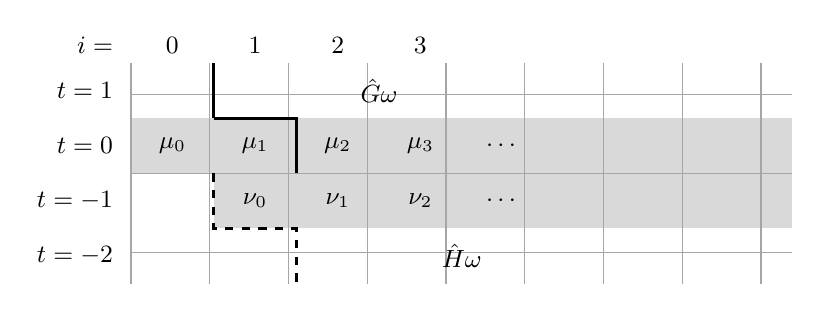
\begin{tikzpicture}[x=1.05cm,y=0.7cm,font=\small]
\foreach \k in {0,...,7} \fill[black!15] (\k-0.5,-0.5) rectangle (\k+0.5,0.5);
\foreach \k in {1,...,7} \fill[black!15] (\k-0.5,-1.5) rectangle (\k+0.5,-0.5);
\draw[black!35,shift={(-0.5,-0.5)}] (0,-2) grid (8,2);
\node at (0,0) {$\mu_0$}; \node at (1,0) {$\mu_1$}; \node at (2,0) {$\mu_2$}; \node at (3,0) {$\mu_3$}; \node at (4,0) {$\cdots$};
\node at (1,-1) {$\nu_0$}; \node at (2,-1) {$\nu_1$}; \node at (3,-1) {$\nu_2$}; \node at (4,-1) {$\cdots$};
\draw[very thick] (0.5,1.5) -- (0.5,0.5);
\draw[very thick] (0.5,0.5) -- (1.5,0.5) -- (1.5,-0.5);
\node at (2.5,1) {$\hat G\omega$};
\draw[very thick,dashed] (0.5,-0.5) -- (0.5,-1.5) -- (1.5,-1.5) -- (1.5,-2.5);
\node at (3.5,-2) {$\hat H\omega$};
\node[left] at (-0.6,1) {$t=1$}; \node[left] at (-0.6,0) {$t=0$}; \node[left] at (-0.6,-1) {$t=-1$}; \node[left] at (-0.6,-2) {$t=-2$};
\foreach \k in {0,1,2,3} \node[above] at (\k,1.5) {$\k$};
\node[above left] at (-0.6,1.5) {$i=$};
\end{tikzpicture}
\caption{The cone code $\omega(Y)$ at the apex $(t,i)=(0,0)$: the entries $\mu_k=Y(0,k)$ and $\nu_k=Y(-1,k+1)$, $k\ge0$ (shaded). The cone codes at the apexes $(0,1)$ and $(0,2)$ are $\sh\omega$ and $\sh^2\omega$. The code $\hat G\omega$ at the apex $(1,1)$ occupies rows $1$ and $0$ (to the right of the solid line), and the code $\hat H\omega$ at the apex $(-1,1)$ occupies rows $-1$ and $-2$ (to the right of the dashed line); both are determined by $\omega$ through \eqref{r30:eq:rec}.}
\label{r30:fig:cone}
\end{figure}

\begin{lemma}\label{r30:lem:I}
\begin{enumerate}
\item For every diagram $Y$,
\[
\omega^{(1,1)}(Y)=\hat G\omega(Y),\quad \omega^{(-1,1)}(Y)=\hat H\omega(Y),\quad \omega^{(0,1)}(Y)=\sh\omega(Y),\quad \omega^{(0,2)}(Y)=\sh^2\omega(Y).
\]
\item For every $\omega\in\A^{\mathbb{N}}$,
\begin{equation}\label{r30:eq:I}
\psi(\hat G\omega)\oplus\psi(\hat H\omega)\oplus\psi(\omega)\oplus\bigl(\psi(\sh\omega)\vee\psi(\sh^2\omega)\bigr)=0.
\end{equation}
\item $\hat G\sh=\sh\hat G$, $\hat H\sh=\sh\hat H$, $\hat GD_1=D_1\hat G$, $\hat HD_1=\hat H$, $\hat HD_2=D_2\hat H$ and $\hat GD_2=\hat G$.
\end{enumerate}
\end{lemma}

\begin{proof}
(1) The last two identities are immediate. By \eqref{r30:eq:rec} at $(0,k+1)$, $Y(1,k+1)=Y(-1,k+1)\oplus Y(0,k)\oplus(Y(0,k+1)\vee Y(0,k+2))=\nu_k\oplus f(\mu_k,\mu_{k+1},\mu_{k+2})$, and $Y(0,k+2)=\mu_{k+2}$; this is $\hat G$. By \eqref{r30:eq:rec} at $(-1,k+2)$, $Y(-2,k+2)=Y(0,k+2)\oplus Y(-1,k+1)\oplus(Y(-1,k+2)\vee Y(-1,k+3))=\mu_{k+2}\oplus f(\nu_k,\nu_{k+1},\nu_{k+2})$, and $Y(-1,k+1)=\nu_k$; this is $\hat H$.

(2) Choose $c$ with $\omega(Y_c)=\omega$. The diagram $Y_{hc}$ satisfies \eqref{r30:eq:rec} at $(0,1)$:
$Y_{hc}(1,1)\oplus Y_{hc}(-1,1)\oplus Y_{hc}(0,0)=Y_{hc}(0,1)\vee Y_{hc}(0,2)$. Now substitute \eqref{r30:eq:psi} and (1).

(3) $\hat G$ and $\hat H$ are given by the same rule at every index $k$, so they commute with $\sh$. The coordinate $\mu_0$ enters $\hat G$ only in the first component of $\hat G(\omega)_0$, through $f(\mu_0,\mu_1,\mu_2)=\mu_0\oplus(\mu_1\vee\mu_2)$, so complementing $\mu_0$ complements the first component of $\hat G(\omega)_0$; this is $\hat GD_1=D_1\hat G$. In that same component $\nu_0\oplus\mu_0$ appears, and $\nu_0$ appears nowhere else in $\hat G$, so $\hat GD_2=\hat G$. The map $\hat H$ does not read $\mu_0$ or $\mu_1$, so $\hat HD_1=\hat H$. Finally, $\nu_0$ enters $\hat H$ only in $\hat H(\omega)_0=(\nu_0,\ \mu_2\oplus\nu_0\oplus(\nu_1\vee\nu_2))$, where complementing it complements both components; this is $\hat HD_2=D_2\hat H$.
\end{proof}

\subsection{Both light edges are permutive}\label{r30:sec:edges}

\begin{proposition}\label{r30:prop:edges}
For every $\omega\in\A^{\mathbb{N}}$, $\psi(D_1\omega)\ne\psi(\omega)$ and $\psi(D_2\omega)\ne\psi(\omega)$.
\end{proposition}

\begin{proof}
Choose $c$ with $\omega(Y_c)=\omega$.

Let $c'$ be $c$ with $y(c_0)$ complemented. Then $\omega(Y_{c'})=D_1\omega$, and $Q=(c,c')$ is a $y$-flip at $0$, with $(U,V)=(0,-2)$ by Lemma~\ref{r30:lem:flips}(2). So $hQ$ has $(U,V)=(0,-2)$. Since $V-U$ is even, Proposition~\ref{r30:prop:profile}(5) gives a middle row at $m=-1$ and $I^+(hQ)=[0,\infty)$, so $\lambda_0(hQ)=0+U=0$. In particular $\Delta_{hQ}(0,0)=1$, that is, $\psi(\omega)\ne\psi(D_1\omega)$.

Let $c'$ be $c$ with $y(c_0)$ and $x(c_1)$ complemented. Then $\omega(Y_{c'})=D_2\omega$, and $Q=(c,c')$ is a $yx$-flip at $0$, so $V(Q)=0$ and $U(Q)\in\{-\infty\}\cup(-\infty,-1]$ (Lemma~\ref{r30:lem:flips}(4)). Then $hQ$ has the same intercepts. If $U(hQ)=-\infty$, then $I^-(hQ)=\Z$ by Proposition~\ref{r30:prop:profile}(3). Otherwise $V-U\ge1$, and by Proposition~\ref{r30:prop:profile}(5) either $I^-(hQ)=(-\infty,t_+-1]$ with $t_+=(V-U+1)/2\ge1$, or $I^-(hQ)=(-\infty,m-1]$ with $m=(V-U)/2\ge1$. In every case $0\in I^-(hQ)$, so $\lambda_0(hQ)=V-0=0$ and $\Delta_{hQ}(0,0)=1$, that is, $\psi(\omega)\ne\psi(D_2\omega)$.
\end{proof}

\begin{corollary}\label{r30:cor:psi}
There is a function $\gamma\colon\A^{\mathbb{N}}\to\{0,1\}$, depending only on the coordinates $0,\dots,R-1$, such that $\psi(\omega)=\mu_0\oplus\gamma(\sh\omega)$ for all $\omega$.
\end{corollary}

\begin{proof}
By Proposition~\ref{r30:prop:edges}, $\psi\oplus\mu_0$ is invariant under $D_1$, so it does not depend on $\mu_0$. It is also invariant under $D_2$, because $D_2$ complements both $\psi$ and $\mu_0$. A function independent of $\mu_0$ and invariant under complementing $(\mu_0,\nu_0)$ is invariant under complementing $\nu_0$. So $\psi\oplus\mu_0$ depends only on $\omega_1,\omega_2,\dots$, and only on $\omega_1,\dots,\omega_R$ because $\psi$ depends only on $\omega_0,\dots,\omega_R$.
\end{proof}

\subsection{The correction term vanishes}\label{r30:sec:gamma}

\begin{lemma}\label{r30:lem:gamma}
Let $\gamma\colon\A^{\mathbb{N}}\to\{0,1\}$ depend on finitely many coordinates, and suppose $\psi(\omega)=\mu_0\oplus\gamma(\sh\omega)$ satisfies \eqref{r30:eq:I}. Then $\gamma\equiv0$.
\end{lemma}

\begin{proof}
For $\theta\in\A^{\mathbb{N}}$ write $\theta_k=(\xi_k,\zeta_k)$. Substitute $\psi$ into \eqref{r30:eq:I} and put $\theta=\sh\omega$, so that $\xi_0=\mu_1(\omega)$ and $\xi_1=\mu_2(\omega)$. Using $\mu_0(\hat G\omega)=\nu_0\oplus\mu_0\oplus(\mu_1\vee\mu_2)$, $\mu_0(\hat H\omega)=\nu_0$, $\sh\hat G=\hat G\sh$ and $\sh\hat H=\hat H\sh$, the terms $\nu_0$ and $\mu_0$ cancel, and \eqref{r30:eq:I} becomes
\begin{equation}\label{r30:eq:star}
\gamma(\hat G\theta)\oplus\gamma(\hat H\theta)\oplus\gamma(\theta)=(\xi_0\vee \xi_1)\oplus\bigl((\xi_0\oplus\gamma(\sh\theta))\vee(\xi_1\oplus\gamma(\sh^2\theta))\bigr).
\end{equation}
This holds for every $\theta\in\A^{\mathbb{N}}$, since $\omega$ is arbitrary.

Three facts are used. (a) $D_1$ and $D_2$ change only $\theta_0$, both complement $\xi_0$, and neither changes $\sh\theta$. (b) The relations of Lemma~\ref{r30:lem:I}(3). (c) Complementing $\xi_0$ while keeping $\xi_1$, $\gamma(\sh\theta)$ and $\gamma(\sh^2\theta)$ fixed changes the right side of \eqref{r30:eq:star} by exactly $\gamma(\sh^2\theta)$. Indeed, $(z\vee e)\oplus(\neg z\vee e)=\neg e$ for bits $z,e$, so the change is $\neg \xi_1\oplus\neg(\xi_1\oplus\gamma(\sh^2\theta))=\gamma(\sh^2\theta)$.

Put $\delta_i=\gamma\oplus(\gamma\circ D_i)$ for $i=1,2$. Evaluate \eqref{r30:eq:star} at $D_1\theta$ and add it to \eqref{r30:eq:star} at $\theta$. By (a)--(c), $\gamma(\hat GD_1\theta)=\gamma(D_1\hat G\theta)$ and $\gamma(\hat HD_1\theta)=\gamma(\hat H\theta)$, so
\begin{equation}\label{r30:eq:one}
\delta_1(\hat G\theta)\oplus\delta_1(\theta)=\gamma(\sh^2\theta).
\end{equation}
In the same way, using $\hat GD_2=\hat G$ and $\hat HD_2=D_2\hat H$,
\begin{equation}\label{r30:eq:two}
\delta_2(\hat H\theta)\oplus\delta_2(\theta)=\gamma(\sh^2\theta).
\end{equation}

Say that a function \emph{depends only on $\theta_0,\dots,\theta_m$} if it takes equal values on sequences that agree in these coordinates; for $m=-1$ this means that it is constant. Let $m\ge-1$ be minimal such that $\gamma$ depends only on $\theta_0,\dots,\theta_m$, and suppose $m\ge0$. Since $D_1$ and $D_2$ act only on $\theta_0$, the functions $\delta_1$ and $\delta_2$ also depend only on $\theta_0,\dots,\theta_m$.

\emph{$\gamma$ does not depend on $\zeta_m$.} For $k\le m$, $\hat G(\theta)_k$ reads only $\xi_k,\xi_{k+1},\xi_{k+2}$ and $\zeta_k$. So the left side of \eqref{r30:eq:one} does not depend on $\zeta_{m+1}$ or $\zeta_{m+2}$, and hence neither does $\gamma(\sh^2\theta)$. Since $(\sh^2\theta)_m=\theta_{m+2}$ and $\sh^2\theta$ ranges over all of $\A^{\mathbb{N}}$, $\gamma$ does not depend on the second component of its coordinate $m$.

\emph{$\gamma$ does not depend on $\xi_m$.} Now $\gamma$, and hence $\delta_2$, depends only on $\theta_0,\dots,\theta_{m-1}$ and $\xi_m$. So $\delta_2(\hat H\theta)$ depends only on $\hat H(\theta)_0,\dots,\hat H(\theta)_{m-1}$ and on the first component of $\hat H(\theta)_m$, which is $\zeta_m$. For $k\le m-1$, $\hat H(\theta)_k$ reads only $\theta_k,\theta_{k+1},\theta_{k+2}$, all with index at most $m+1$. So the left side of \eqref{r30:eq:two} does not depend on $\theta_{m+2}$, and hence neither does $\gamma(\sh^2\theta)$. Since $\gamma(\sh^2\theta)$ depends on $\theta_{m+2}$ only through $\xi_{m+2}$, $\gamma$ does not depend on the first component of its coordinate $m$.

Thus $\gamma$ depends only on $\theta_0,\dots,\theta_{m-1}$, contradicting the minimality of $m$. Hence $m=-1$ and $\gamma$ is constant. Then $\delta_1\equiv0$, and \eqref{r30:eq:one} gives $\gamma(\sh^2\theta)=0$, so $\gamma\equiv0$.
\end{proof}

\subsection{Parity and the proof of Theorem~\ref{thm:rigidity30}}\label{r30:sec:conclusion}

\begin{proposition}\label{r30:prop:trivial}
If $h\in\Aut(X_F)$ satisfies $e^+(h)=e^-(h)=0$, then $h=\mathrm{id}$.
\end{proposition}

\begin{proof}
By Corollary~\ref{r30:cor:psi} and Lemmas~\ref{r30:lem:I}(2) and~\ref{r30:lem:gamma}, $\psi(\omega)=\mu_0$. By \eqref{r30:eq:psi}, $Y_{hc}(t,i)=\mu_0(\omega^{(t,i)}(Y_c))=Y_c(t,i)$ for all $(t,i)$. So $Y_{hc}=Y_c$, and $hc=c$ for every $c$.
\end{proof}

\begin{lemma}\label{r30:lem:parity}
For every $h\in\Aut(X_F)$, $e^+(h)\equiv e^-(h)\pmod 2$.
\end{lemma}

\begin{proof}
For a cell $s\in\A$ let $\bar s=s^{\Z}$ be the constant configuration. Since $f(y,y,y)=y\oplus(y\vee y)=0$, we have $F(\overline{(x,y)})=\overline{(y,x)}$. So $F$ permutes the four constant configurations as the transposition exchanging $\overline{(0,1)}$ and $\overline{(1,0)}$, fixing the other two. Every $h\in\Aut(X_F)$ commutes with $\sh$, so it maps the four $\sh$-fixed points bijectively to themselves, and the induced permutation commutes with that of $F$. The centralizer in $\Sym(4)$ of a transposition $(\alpha\,\beta)$ is $\langle(\alpha\,\beta)\rangle\times\langle(\alpha'\,\beta')\rangle$, where $\{\alpha',\beta'\}$ is the complement of $\{\alpha,\beta\}$. Every element of this group has order at most $2$, so $h^2$ fixes every constant configuration.

Suppose $e^+(h)+e^-(h)$ is odd. Put $a=-(e^+(h)+e^-(h)+1)/2$ and $b=(e^+(h)-e^-(h)-1)/2$, which are integers. By Corollary~\ref{r30:cor:offsets}, $(e^+,e^-)(\sh^aF^b)=(b-a,-a-b)=(e^+(h),e^-(h)+1)$, so $h_1=F^{-b}\sh^{-a}h$ has offsets $(0,-1)$. Then $h_1^2$ has offsets $(0,-2)=(e^+,e^-)(\sh F)$, so $h_1^2(\sh F)^{-1}$ has offsets $(0,0)$, and $h_1^2=\sh F$ by Proposition~\ref{r30:prop:trivial}. But $h_1^2$ fixes every constant configuration, while $\sh F$ exchanges $\overline{(0,1)}$ and $\overline{(1,0)}$. This is a contradiction.
\end{proof}

\begin{proof}[Proof of Theorem~\ref{thm:rigidity30}]
Let $h\in\Aut(X_F)$. By Lemma~\ref{r30:lem:parity}, $e^+(h)+e^-(h)$ is even, so $a=-\tfrac12(e^+(h)+e^-(h))$ and $b=\tfrac12(e^+(h)-e^-(h))$ are integers, and $(e^+,e^-)(\sh^aF^b)=(b-a,-a-b)=(e^+(h),e^-(h))$. Hence $h_0=F^{-b}\sh^{-a}h$ has $e^+(h_0)=e^-(h_0)=0$, so $h_0=\mathrm{id}$ by Proposition~\ref{r30:prop:trivial}, and $h=\sh^aF^b$. Uniqueness of $(a,b)$ and $\langle\sh,F\rangle\cong\Z^2$ are Corollary~\ref{r30:cor:offsets}(4). By Lemma~\ref{lem:spacetime}, this describes $\Aut(X_{F_{30}})$.
\end{proof}

\begin{remark}
The properties of rule $30$ used are the following: the second-order rule is permutive in the previous row and in the left neighbour, so it satisfies Lemma~\ref{r30:lem:R}; the maximum principle (Lemma~\ref{r30:lem:max}), which uses only Lemmas~\ref{r30:lem:onset} and~\ref{r30:lem:flips}; the strong connectivity of the light-speed window graph $\Lambda_M$ (Lemma~\ref{r30:lem:lambda}), whose proof uses the specific form $a\oplus(b\vee c)$ only through the stationary loop \eqref{r30:eq:loop}; the cone identity \eqref{r30:eq:I} forces the correction to vanish (Lemma~\ref{r30:lem:gamma}); and $f(y,y,y)=0$, which is used for the parity. Permutivity in the right argument, which rule $30$ lacks, is never used.
\end{remark}


\section{Permutive automata of any radius}\label{sec:general}

In this section we extend Theorem~\ref{thm:rigidity30} to second-order automata of any radius $r\ge1$ over $\F_2=\{0,1\}$ whose rule is permutive in its leftmost variable. Most of the proof carries over once the speed $1$ of the fronts is replaced by $r$, and we state each such step at radius $r$ with its proof, or with a precise reference to the proof for rule $30$ and the indices that change. Three steps need new arguments. The correction term is removed by a descent on the largest coordinates that it reads, which works when a second derivative of the rule reaches far enough to the right (Section~\ref{gen:sec:strip}). The strong connectivity of the light-speed window graph is reduced to a finite certificate that covers all window lengths at once (Section~\ref{gen:sec:tower}). And the parity step is replaced by an orbit-counting obstruction on spatially periodic points (Section~\ref{gen:sec:index}), because the offsets determine an automorphism only up to an index $2r$. The elementary rules are treated as the case $r=1$ in Section~\ref{sec:permutive}.

\subsection{Setting, hypotheses and results}\label{gen:sec:setting}

Fix $r\ge1$ and a Boolean function $g\colon\{0,1\}^{2r}\to\{0,1\}$. Put
\begin{equation}\label{gen:eq:f}
f(y_{i-r},\dots,y_{i+r})=y_{i-r}\oplus g(\xi_0,\dots,\xi_{2r-1}),\qquad \xi_k=y_{i-r+1+k}\ \ (0\le k\le 2r-1),
\end{equation}
and define $F$ on $\A^{\Z}$, $\A=\{0,1\}^2$ with cells $(x,y)$, by
\begin{equation}\label{gen:eq:F}
F(c)_i=\bigl(y_i,\;x_i\oplus f(y_{i-r},\dots,y_{i+r})\bigr).
\end{equation}
For $r=1$ this is \eqref{eq:F} for an elementary rule of the form $f(a,b,c)=a\oplus g(b,c)$; rule $30$ is $g(b,c)=b\vee c$. The map $F$ is reversible, with $F^{-1}(c)_i=\bigl(y_i\oplus f(x_{i-r},\dots,x_{i+r}),\,x_i\bigr)$, and $F$ and $F^{-1}$ have radius $r$. Lemma~\ref{lem:spacetime} holds for every reversible cellular automaton, so $\Aut(X_F)$ is the group of invertible block maps commuting with $F$, and $\langle\sh,\tau\rangle$ corresponds to $\langle\sh,F\rangle$. From now on the letter $g$ denotes this function, and automorphisms are denoted $h,h_1,\dots$, as before.

For $\varphi\colon\{0,1\}^{2r}\to\{0,1\}$ and $0\le j\le 2r-1$, let $\xi^{(j)}$ be $\xi$ with its coordinate $\xi_j$ complemented, and $\partial_j\varphi(\xi)=\varphi(\xi)\oplus\varphi(\xi^{(j)})$. Then $\partial_j\varphi\equiv0$ if and only if $\varphi$ does not depend on $\xi_j$, $\partial_j\partial_k=\partial_k\partial_j$ and $\partial_j\partial_j=0$. We write $\mathbf 1=(1,\dots,1)$.

\begin{definition}[light-speed window graph]\label{gen:def:lambda}
Fix $M\ge0$. The graph $\Lambda_M$ has vertex set $\A^{M+1}$ and, for every vertex $\omega=\omega_0\cdots\omega_M$ and every word $\iota=\iota_1\cdots\iota_{2r}\in\A^{2r}$, an edge $\omega\to\omega\cdot\iota$, where
\[
(\omega\cdot\iota)_k=F(\tilde c)_{p+r+k}\qquad(0\le k\le M)
\]
and $\tilde c$ is any configuration with $\tilde c_{p+k}=\omega_k$ for $0\le k\le M$ and $\tilde c_{p+M+j}=\iota_j$ for $1\le j\le 2r$. Since $F$ has radius $r$, the cells $F(\tilde c)_i$ with $p+r\le i\le p+r+M$ read only $\tilde c$ on $[p,p+M+2r]$, so $\omega\cdot\iota$ depends neither on $p$ nor on the other cells of $\tilde c$. A vertex is the word of one configuration on a front cell $p$ and the $M$ cells ahead of it, and an edge advances the front by $r$ sites, at the speed of light. For $r=1$ this is the graph $\Lambda_M$ of Section~\ref{r30:sec:window}.
\end{definition}

The cellwise complement is $\kappa(c)_i=(1\oplus x_i,\,1\oplus y_i)$. We call $g$ \emph{self-dual} if $g(\xi\oplus\mathbf 1)=g(\xi)\oplus1$ for every $\xi$.

\begin{lemma}\label{gen:lem:kappa}
$\kappa$ is an involution commuting with $\sh$, and $\kappa F=F\kappa$ if and only if $g$ is self-dual.
\end{lemma}

\begin{proof}
The first statement is clear. By \eqref{gen:eq:F}, $F(\kappa c)_i=(1\oplus y_i,\,1\oplus x_i\oplus f(y\oplus\mathbf 1))$ and $\kappa F(c)_i=(1\oplus y_i,\,1\oplus x_i\oplus f(y))$, where $y$ stands for $(y_{i-r},\dots,y_{i+r})$. By \eqref{gen:eq:f}, $f(y\oplus\mathbf 1)\oplus f(y)=1\oplus g(\xi\oplus\mathbf 1)\oplus g(\xi)$. This vanishes for all $y$ exactly when $g$ is self-dual.
\end{proof}

\paragraph{Spatially periodic points.} For $n\ge1$ let $\mathrm{Per}_n=\{c\in\A^{\Z}:\sh^nc=c\}$, a finite set of $4^n$ points, and $\mathrm{Per}=\bigcup_n\mathrm{Per}_n$. The group $\Z^2$ acts on $\mathrm{Per}$ by $(a,b)\cdot c=\sh^aF^bc$, and $\mathrm{Stab}(c)=\{(a,b):\sh^aF^bc=c\}$.

\begin{lemma}\label{gen:lem:stab}
Let $c\in\mathrm{Per}$ have least spatial period $n$. Then $\mathrm{Stab}(c)\cap(\Z\times\{0\})=n\Z\times\{0\}$, and $\mathrm{Stab}(c)$ has finite index in $\Z^2$. All points of a $\Z^2$-orbit have the same stabiliser. If $\mathcal L$ is a subgroup of finite index and $\mathcal L\cap(\Z\times\{0\})=n\Z\times\{0\}$, then every orbit with stabiliser $\mathcal L$ consists of points of least period $n$. In particular the number $k(\mathcal L)$ of $\Z^2$-orbits in $\mathrm{Per}$ whose stabiliser is exactly $\mathcal L$ is finite, and it is computed exactly by enumerating the points of least period $n$ in $\mathrm{Per}_n$.
\end{lemma}

\begin{proof}
The first statement is the definition of the least period. $F$ commutes with $\sh$ and is injective, so it permutes the finite set $\mathrm{Per}_n$, and $F^\ell c=c$ for some $\ell\ge1$. So $(n,0),(0,\ell)\in\mathrm{Stab}(c)$. Stabilisers are constant on orbits because $\Z^2$ is abelian. The rest follows.
\end{proof}

\begin{definition}[index condition]\label{gen:def:index}
For a subgroup $\mathcal L\subseteq\Z^2$ of finite index let $k(\mathcal L)$ be the number of $\Z^2$-orbits in $\mathrm{Per}$ whose stabiliser is exactly $\mathcal L$ (Lemma~\ref{gen:lem:stab}). For a prime $q$ dividing $2r$ put
\[
a_q=0\ \text{ if $q$ is odd},\qquad a_2=r\bmod2 .
\]
Condition $(\mathrm{I})_q$ is: \emph{there is a subgroup $\mathcal L\subseteq\Z^2$ of finite index with $q\nmid k(\mathcal L)$ and $(a_q,1)\notin q\Z^2+\mathcal L$.}
\end{definition}

Since $q\mid0$, a subgroup witnessing $(\mathrm{I})_q$ is the stabiliser of at least one orbit. We call such an $\mathcal L$ a \emph{witness}.

\begin{definition}[hypotheses]\label{gen:def:hyp}
\begin{itemize}
\item[(N)] \emph{Stripping condition.} $\partial_0g$ is not constant, and
\[
J(g)=\max\{j\in[1,2r-1]:\ \partial_0\partial_jg\not\equiv0\}\quad\text{satisfies}\quad J(g)\ge r.
\]
(Since $\partial_0\partial_0g=0$, $\partial_0g$ is non-constant exactly when this set is nonempty.) For $r\ge2$ this is strictly stronger than non-affineness of $g$.
\item[(D)] \emph{Not self-dual.} $g(\xi\oplus\mathbf 1)\ne g(\xi)\oplus1$ for some $\xi$; equivalently (Lemma~\ref{gen:lem:kappa}), $\kappa$ does not commute with $F$.
\item[($\Lambda$)] \emph{Light-speed connectivity.} $\Lambda_M$ is strongly connected for every $M\ge0$.
\item[(I)] \emph{Index condition.} $(\mathrm{I})_q$ holds for every prime $q$ dividing $2r$.
\end{itemize}
\end{definition}

For $r=1$, $\partial_0\partial_1g$ is the coefficient of $\xi_0\xi_1$ in the algebraic normal form of $g$, so (N) says that $f$ is not affine. For $r=2$, \textup{(N)} holds for $64\,512$ of the $65\,504$ non-affine $g$, and \textup{(N)} and \textup{(D)} both hold for $64\,288$ of them. Hypothesis ($\Lambda$) is established by the finite computation of Section~\ref{gen:sec:tower}, a sufficient certificate that covers all $M$ at once, and (I) by enumerating spatially periodic points (Section~\ref{gen:sec:index}). Both computations are semi-decision procedures: a positive answer proves the hypothesis, and a negative answer at a given size proves nothing.

The offsets $e^\pm$ below are those of Proposition~\ref{gen:prop:offsets}. They are the radius-$r$ versions of the offsets of Corollary~\ref{r30:cor:offsets}.

\begin{theorem}\label{gen:main}
Assume \textup{(N)}, \textup{(D)}, \textup{($\Lambda$)} and \textup{(I)}. Then every invertible block map $h$ commuting with $F$ equals $\sh^aF^b$ for exactly one $(a,b)\in\Z^2$, namely
\[
a=-\tfrac12\bigl(e^+(h)+e^-(h)\bigr),\qquad b=\tfrac1{2r}\bigl(e^+(h)-e^-(h)\bigr).
\]
Hence $\Aut(X_F)=\langle\sh,F\rangle\cong\Z^2$.
\end{theorem}

The next theorem records what each hypothesis contributes. Write $e=(e^+,e^-)$.

\begin{theorem}\label{gen:structure}
\begin{enumerate}
\item[(a)] The map $(a,b)\mapsto\sh^aF^b$ is an isomorphism $\Z^2\to\langle\sh,F\rangle$; this needs no hypothesis. Assume \textup{($\Lambda$)}. Then every $h\in\Aut(X_F)$ has offsets $e^\pm(h)\in\Z$ (Proposition~\ref{gen:prop:offsets}), and $e^+,e^-$ are homomorphisms $\Aut(X_F)\to\Z$ with
\[
e(\sh^aF^b)=(rb-a,\ -a-rb).
\]
The image of $\langle\sh,F\rangle$ under $e$ is $L=\{(m,n)\in\Z^2:m\equiv n\pmod{2r}\}$. It has index $2r$ in $\Z^2$, and $(m,n)\mapsto m-n$ induces $\Z^2/L\cong\Z/2r$.
\item[(b)] Assume \textup{($\Lambda$)} and \textup{(N)}. Then $\ker e=\{\mathrm{id}\}$ if \textup{(D)} holds, and $\ker e=\{\mathrm{id},\kappa\}$ if $g$ is self-dual. Consequently, under \textup{($\Lambda$)}, \textup{(N)} and \textup{(D)}, $e$ is injective, $\Aut(X_F)\cong\Z^2$, and $\langle\sh,F\rangle$ has index dividing $2r$ in $\Aut(X_F)$, with cyclic quotient.
\item[(c)] If $g$ is self-dual, then $\kappa\in\Aut(X_F)$ has order $2$, commutes with $\sh$ and $F$, and does not lie in $\langle\sh,F\rangle$; so \textup{(D)} is necessary for $\Aut(X_F)=\langle\sh,F\rangle$. If moreover \textup{($\Lambda$)} and \textup{(N)} hold, then $\kappa$ is central in $\Aut(X_F)$.
\item[(d)] Assume \textup{($\Lambda$)}, \textup{(N)} and \textup{(D)}, and let $q$ be a prime dividing $2r$. Then $q$ divides $[\Aut(X_F):\langle\sh,F\rangle]$ if and only if $h_1^q=\sh^aF$ for some $h_1\in\Aut(X_F)$ and some $a\in\Z$, and in that case necessarily $a\equiv-r\equiv a_q\pmod q$. Condition $(\mathrm{I})_q$ rules out $h_1^q=\sh^aF$ with $a\equiv a_q\pmod q$, without any further hypothesis. Hence $(\mathrm{I})_q$ implies that $q$ does not divide the index, and \textup{(I)} removes the index entirely.
\end{enumerate}
\end{theorem}

\begin{remark}[scope]\label{gen:rem:scope}
\begin{enumerate}
\item For $r=1$, (N) is non-affineness, and (D) then holds automatically (Section~\ref{pm:sec:audit}). The four hypotheses hold for the eight non-affine left-permutive elementary rules (Section~\ref{sec:permutive}).
\item The reflection $\mathrm{rev}(c)_i=c_{-i}$ conjugates $F$ to the automaton of the reflected rule $f^r(y_{i-r},\dots,y_{i+r})=f(y_{i+r},\dots,y_{i-r})$, since by \eqref{gen:eq:F},
\[
\mathrm{rev}\,F\,\mathrm{rev}(c)_i=F(\mathrm{rev}\,c)_{-i}=\bigl(y_i,\,x_i\oplus f(y_{i+r},\dots,y_{i-r})\bigr).
\]
It satisfies $\mathrm{rev}\,\sh\,\mathrm{rev}=\sh^{-1}$, so it maps $\langle\sh,F\rangle$ onto the corresponding group, and it preserves radii. So the theorem also applies to rules permutive in their rightmost variable, after reflection. Rules permutive in both outer variables are included when the hypotheses hold; an example with $r=2$ is in Table~\ref{gen:tab:r2}.
\item If $g$ is affine, then $\partial_0g$ is constant and (N) fails. This is not an artefact of the method: for rule $150$, the map $\mathrm{id}+\sh F$ is an automorphism outside $\langle\sh,F\rangle$ (Remark~\ref{pm:rem:linear}).
\end{enumerate}
\end{remark}

The hypotheses enter as follows. ($\Lambda$) gives the offsets (Sections~\ref{gen:sec:front}--\ref{gen:sec:allpairs}). (N) forces the correction term to be constant (Section~\ref{gen:sec:strip}). (D) excludes the constant $1$, that is, $\kappa$ (Section~\ref{gen:sec:kernel}). (I) removes the remaining index (Section~\ref{gen:sec:index}). The proofs of the two theorems are in Section~\ref{gen:sec:proofs}.

\medskip
\noindent\textbf{Conventions.} Those of Section~\ref{sec:rigidity30}: $[S]\in\{0,1\}$ is the truth value of $S$, intervals are intervals of integers, and $-\infty+k=-\infty<n$, $\max\emptyset=-\infty$.

\subsection{Diagrams, profiles and flips}\label{gen:sec:profiles}

The definitions of Section~\ref{r30:sec:diagrams} are used without change: the diagram $Y_c(t,i)$ is the $y$-bit of $F^t(c)$ at site $i$, so that the $x$-row of $F^t(c)$ is row $t-1$ and $c_i=(Y_c(-1,i),Y_c(0,i))$; pairs $Q=(c,c')$ are ordered pairs of distinct configurations that agree far to the right; $\Delta_Q=Y_c\oplus Y_{c'}$; and $\rho(c)_i=(y_i,x_i)$. By \eqref{gen:eq:F}, every diagram satisfies
\begin{equation}\label{gen:eq:rec}
Y(t+1,i)\oplus Y(t-1,i)\oplus Y(t,i-r)=g\bigl(Y(t,i-r+1),\dots,Y(t,i+r)\bigr)\qquad\text{for all }(t,i).
\end{equation}
This is an exclusive or in each of $Y(t+1,i)$, $Y(t-1,i)$ and $Y(t,i-r)$, so two consecutive rows determine the diagram, and $c\mapsto Y_c$ is a bijection onto the solutions of \eqref{gen:eq:rec}. Equations \eqref{r30:eq:transl} and \eqref{r30:eq:rows} hold as stated, since their proofs do not involve the radius. The computation before \eqref{r30:eq:rho}, with the formula for $F^{-1}$ above, gives $\rho F\rho=F^{-1}$ and \eqref{r30:eq:rho}, so $h\mapsto\rho h\rho$ is an automorphism of $\Aut(X_F)$. If rows $t-1$ and $t$ of $\Delta_Q$ vanish to the right of $s$, then by \eqref{gen:eq:rec} rows $t+1$ and $t-2$ vanish to the right of $s+r$; hence every row of $\Delta_Q$ vanishes far to the right, and the profile $\lambda_t=\lambda_t(Q)=\max\{i:\Delta_Q(t,i)=1\}\in\Z\cup\{-\infty\}$ is defined.

\begin{lemma}\label{gen:lem:R}
For every pair and every $t$:
\begin{enumerate}
\item $\lambda_{t+1}\le\max(\lambda_{t-1},\lambda_t+r)$, with equality if $\lambda_{t-1}\ne\lambda_t+r$;
\item $\lambda_{t-1}\le\max(\lambda_{t+1},\lambda_t+r)$, with equality if $\lambda_{t+1}\ne\lambda_t+r$.
\end{enumerate}
\end{lemma}

\begin{proof}
By \eqref{gen:eq:rec}, $\Delta(t+1,i)=\Delta(t-1,i)\oplus\Delta(t,i-r)\oplus D_i$, where $D_i$ is the difference of the two values of $g$, which read row $t$ on $[i-r+1,i+r]$. Let $m=\max(\lambda_{t-1},\lambda_t+r)$. For $i\ge\lambda_t+r$ we have $i-r+1>\lambda_t$, so $D_i=0$. For $i>m$ all three terms vanish. If $m$ is finite, then $D_m=0$, $\Delta(t-1,m)=[m=\lambda_{t-1}]$ and $\Delta(t,m-r)=[m=\lambda_t+r]$. At least one of these is $1$, and both are $1$ only if $\lambda_{t-1}=\lambda_t+r$. This proves (1). Part (2) is the same argument for \eqref{gen:eq:rec} solved for $Y(t-1,i)$, which has the same form with $t\pm1$ exchanged.
\end{proof}

\begin{proposition}\label{gen:prop:profile}
Let $Q$ be a pair, and put
\[
I^+=\{t:\lambda_t\ne-\infty,\ \lambda_{t-1}<\lambda_t+r\},\qquad I^-=\{t:\lambda_t\ne-\infty,\ \lambda_{t+1}<\lambda_t+r\}.
\]
\begin{enumerate}
\item No two consecutive $\lambda_t$ equal $-\infty$.
\item If $t\in I^+$, then $\lambda_{t+1}=\lambda_t+r$ and $t+1\in I^+$. If $t\in I^-$, then $\lambda_{t-1}=\lambda_t+r$ and $t-1\in I^-$. The sets $I^\pm$ are disjoint, and every element of $I^-$ is smaller than every element of $I^+$.
\item $\Z\setminus(I^+\cup I^-)$ has at most one element. If $m$ is such an element (a \emph{middle row}), then $m-1\in I^-$, $m+1\in I^+$, and $\lambda_{m-1}=\lambda_{m+1}\ge\lambda_m+r$. If $I^+=\emptyset$ then $I^-=\Z$, and if $I^-=\emptyset$ then $I^+=\Z$.
\item Put $U=\lambda_t-rt$ for $t\in I^+$ and $V=\lambda_t+rt$ for $t\in I^-$, with $U=-\infty$ if $I^+=\emptyset$ and $V=-\infty$ if $I^-=\emptyset$ (the \emph{forward} and \emph{backward intercepts}). Then $\lambda_t\le\max(rt+U,\,V-rt)$ for every $t$; that is, $\Delta_Q(t,i)=1$ implies $i-rt\le U$ or $i+rt\le V$.
\item Suppose $U,V$ are finite. If $2r\mid V-U$, there is a middle row $m=(V-U)/2r$, and $I^+=[m+1,\infty)$, $I^-=(-\infty,m-1]$. Otherwise there is no middle row, and $I^+=[t_+,\infty)$, $I^-=(-\infty,t_+-1]$ with $t_+=\lceil(V-U)/2r\rceil$. In particular $I^+$ and $I^-$ are determined by $(U,V)$, also when $U$ or $V$ is $-\infty$.
\item For every $t$, $U\le\max\bigl(\lambda_t-rt,\ \lambda_{t-1}-r(t+1)\bigr)$ and $V\le\max\bigl(\lambda_t+rt,\ \lambda_{t+1}+r(t-1)\bigr)$.
\end{enumerate}
\end{proposition}

\begin{proof}
This is the proof of Proposition~\ref{r30:prop:profile} with the step $1$ replaced by $r$, using Lemma~\ref{gen:lem:R}. We give the points where $r$ enters.
(1) Two vanishing consecutive rows give $c=c'$.
(2) If $t\in I^+$, Lemma~\ref{gen:lem:R}(1) gives $\lambda_{t+1}=\lambda_t+r$, and then $\lambda_t<\lambda_{t+1}+r$, so $t+1\in I^+$. Symmetrically for $I^-$. If $t\in I^+$ then $\lambda_{t+1}=\lambda_t+r$, so $t\notin I^-$; and $a\in I^+$, $b\in I^-$, $a\le b$ would give $b\in I^+$.
(3) Let $t\notin I^+\cup I^-$. If $\lambda_t=-\infty$, then $\lambda_{t\pm1}$ are finite by (1), so $t+1\in I^+$ and $t-1\in I^-$. If $\lambda_t$ is finite, then $\lambda_{t-1}\ge\lambda_t+r$ and $\lambda_{t+1}\ge\lambda_t+r$, which give $t-1\in I^-$ and $t+1\in I^+$. Uniqueness and the last sentence follow from (2) as before. For the values: if $\lambda_{m-1}\ne\lambda_m+r$, Lemma~\ref{gen:lem:R}(1) gives $\lambda_{m+1}=\max(\lambda_{m-1},\lambda_m+r)=\lambda_{m-1}$; if $\lambda_{m-1}=\lambda_m+r$, then $\lambda_m+r\le\lambda_{m+1}\le\max(\lambda_{m-1},\lambda_m+r)=\lambda_m+r$.
(4) On $I^\pm$ this is the definition. For a middle row, $\lambda_m\le\lambda_{m-1}-r=V-rm$.
(5) If there is no middle row, $I^-=(-\infty,t_+-1]$ and $I^+=[t_+,\infty)$. Now $t_+\in I^+$ reads $V-r(t_+-1)<rt_++U+r$, that is $V-U<2rt_+$, and $t_+-1\in I^-$ reads $rt_++U<V-r(t_+-1)+r$, that is $V-U>2r(t_+-1)$. If there is a middle row $m$, then $\lambda_{m+1}=\lambda_{m-1}$ reads $r(m+1)+U=V-r(m-1)$, that is $V-U=2rm$. Divisibility of $V-U$ by $2r$ decides which case occurs. If $U=-\infty$ then $I^-=\Z$, and if $V=-\infty$ then $I^+=\Z$, by (3).
(6) Put $\mu_t=\max(\lambda_t-rt,\ \lambda_{t-1}-r(t+1))$. By Lemma~\ref{gen:lem:R}(1), $\lambda_{t+1}-r(t+1)\le\max(\lambda_{t-1}-r(t+1),\lambda_t-rt)\le\mu_t$, and $\lambda_t-r(t+2)<\mu_t$, so $\mu_{t+1}\le\mu_t$. If $t-1\in I^+$, then $\mu_t=\max(U,U-2r)=U$. Hence $U\le\mu_t$ for all $t$. The statement for $V$ follows in the same way from Lemma~\ref{gen:lem:R}(2), with $\nu_t=\max(\lambda_t+rt,\lambda_{t+1}+r(t-1))$, which is nondecreasing and equals $V$ when $t+1\in I^-$.
\end{proof}

\begin{lemma}\label{gen:lem:transl}
For every pair $Q$ and all $j,k\in\Z$: $U(F^kQ)=U(Q)+rk$ and $V(F^kQ)=V(Q)-rk$; $U(\sh^jQ)=U(Q)-j$ and $V(\sh^jQ)=V(Q)-j$; $U(\rho Q)=V(Q)+r$ and $V(\rho Q)=U(Q)-r$. The value $-\infty$ is preserved in each case.
\end{lemma}

\begin{proof}
$\lambda_t(F^kQ)=\lambda_{t+k}(Q)$ and $\lambda_t(\sh^jQ)=\lambda_t(Q)-j$, so $I^\pm(F^kQ)=I^\pm(Q)-k$ and $I^\pm(\sh^jQ)=I^\pm(Q)$; for $t\in I^+(F^kQ)$, $\lambda_{t+k}-rt=U+rk$. By \eqref{r30:eq:rho}, $\lambda_t(\rho Q)=\lambda_{-1-t}(Q)$, so $t\in I^+(\rho Q)$ iff $-1-t\in I^-(Q)$, and then $\lambda_t(\rho Q)-rt=V-r(-1-t)-rt=V+r$; similarly $t\in I^-(\rho Q)$ iff $-1-t\in I^+(Q)$, and then $\lambda_t(\rho Q)+rt=U+r(-1-t)+rt=U-r$.
\end{proof}

A pair $(c,c')$ is a \emph{front pair at $p$} if $c_i=c'_i$ for $i>p$, $y(c_p)\ne y(c'_p)$ and $x(c_p)=x(c'_p)$; equivalently, $\lambda_0=p>\lambda_{-1}$. The \emph{$y$-flip} and the \emph{$x$-flip at $j$} complement the bit $y(c_j)$, respectively $x(c_j)$. The \emph{$yx$-flip at $j$} complements both $y(c_j)$ and $x(c_{j+r})$.

\begin{lemma}\label{gen:lem:flips}
\begin{enumerate}
\item If $Q$ is a front pair at $p$, then $U(Q)=p$, and $F^tQ$ is a front pair at $p+rt$ for every $t\ge0$.
\item A $y$-flip at $j$ is a front pair at $j$, and $(U,V)=(j,\,j-2r)$.
\item If $Q$ is an $x$-flip at $j$, then $FQ$ is a front pair at $j$, and $(U,V)=(j-r,\,j-r)$.
\item A $yx$-flip at $j$ has $V=j$, and either $U=-\infty$ or $U\le j-1$.
\end{enumerate}
\end{lemma}

\begin{proof}
(1) $\lambda_{-1}<\lambda_0<\lambda_0+r$, so $0\in I^+$ and $U=p$. By Proposition~\ref{gen:prop:profile}(2), $\lambda_t=p+rt$ for $t\ge0$, so $\lambda_0(F^tQ)=p+rt>p+r(t-1)=\lambda_{-1}(F^tQ)$ for $t\ge1$.
(2) $\lambda_0=j$ and $\lambda_{-1}=-\infty$, so $U=j$. Lemma~\ref{gen:lem:R}(2) at $t=-1$ gives $\lambda_{-2}=\max(\lambda_0,\lambda_{-1}+r)=j$, and $\lambda_{-1}<\lambda_{-2}+r$, so $-2\in I^-$ and $V=j-2r$.
(3) $\lambda_{-1}=j$ and $\lambda_0=-\infty$. Lemma~\ref{gen:lem:R}(1) at $t=0$ gives $\lambda_1=j$. So $FQ$ is a front pair at $j$, $1\in I^+$ and $U=j-r$; and $\lambda_0<\lambda_{-1}+r$ gives $-1\in I^-$ and $V=j-r$.
(4) $\lambda_0=j$ and $\lambda_{-1}=j+r$, so $\lambda_0<\lambda_{-1}+r$, $-1\in I^-$ and $V=\lambda_{-1}-r=j$. For $i>j+r$, all three terms of $\Delta(1,i)=\Delta(-1,i)\oplus\Delta(0,i-r)\oplus D_i$ vanish, since $i-r>j=\lambda_0$. At $i=j+r$, $D_{j+r}$ reads row $0$ on $[j+1,j+2r]$, where $\Delta$ vanishes, so $\Delta(1,j+r)=1\oplus1\oplus0=0$. Hence $\lambda_1\le j+r-1$, and Proposition~\ref{gen:prop:profile}(6) at $t=1$ gives $U\le\max(\lambda_1-r,\lambda_0-2r)\le j-1$.
\end{proof}

By Proposition~\ref{gen:prop:profile}(5), statement (4) determines $I^\pm$ of every pair with the intercepts of a $yx$-flip at $j$. This is used in Proposition~\ref{gen:prop:edges}.

\begin{proposition}\label{gen:prop:Z2}
$(a,b)\mapsto\sh^aF^b$ is an isomorphism $\Z^2\to\langle\sh,F\rangle$.
\end{proposition}

\begin{proof}
It is a surjective homomorphism since $\sh F=F\sh$. Let $Q$ be a $y$-flip at $0$, so $(U,V)=(0,-2r)$. By Lemma~\ref{gen:lem:transl}, $\sh^aF^bQ$ has $(U,V)=(rb-a,\,-2r-a-rb)$. If $\sh^aF^b=\mathrm{id}$, then $rb-a=0=a+rb$, so $a=b=0$.
\end{proof}

\subsection{The front offset}\label{gen:sec:front}

In this subsection $h$ is an invertible block map commuting with $F$, $R\ge1$ bounds the radii of $h$ and $h^{-1}$, and
\[
M_R=2r(R+1)+2R .
\]
For $r=1$, $M_R=4R+2$ as in Section~\ref{r30:sec:front}.

\begin{lemma}[onset]\label{gen:lem:onset}
Let $P$ be a front pair at $p$, and let $t_+=\min I^+(hP)$. Then $U(hP)$ is finite, $t_+\le\lfloor R/r\rfloor+1$, and $|U(hP)-p|\le R$. In particular $\lambda_t(hP)=rt+U(hP)$ for every $t\ge R+1$, and for $r\ge2$ already $t_+\le R$.
\end{lemma}

\begin{proof}
Write $\lambda_t=\lambda_t(hP)$ and $P=(c,c')$, and let $t\ge0$. By Lemma~\ref{gen:lem:flips}(1), $F^tP$ is a front pair at $p+rt$. By \eqref{r30:eq:rows}, rows $t-1$ and $t$ of $\Delta_{hP}$ record the $x$- and $y$-differences of $h(F^tc)$ and $h(F^tc')$. These agree beyond $p+rt+R$, so $\lambda_t,\lambda_{t-1}\le p+rt+R$; and since $h^{-1}$ has radius at most $R$, they differ somewhere in $[p+rt-R,p+rt+R]$, so $\max(\lambda_t,\lambda_{t-1})\ge p+rt-R$.

Suppose $t_+\ge2$ (including $t_+=\infty$ if $I^+=\emptyset$). By Proposition~\ref{gen:prop:profile}(2),(3), every $t\le t_+-2$ lies in $I^-$, and $t_+-1$ lies in $I^-$ or is the middle row, so $\lambda_t\le V-rt$ for $t\le t_+-1$, with $V=V(hP)$ finite. As $-1\in I^-$, the upper bound at $t=0$ gives $V+r=\lambda_{-1}\le p+R$. For $1\le t\le t_+-1$,
\[
p+rt-R\le\max(\lambda_t,\lambda_{t-1})\le V-r(t-1)\le p+R-rt,
\]
so $t\le R/r$. If $t_+=\infty$ this fails at $t=\lfloor R/r\rfloor+1$. Otherwise $t=t_+-1$ gives $t_+\le\lfloor R/r\rfloor+1$. In all cases $U$ is finite and $t_+\le\lfloor R/r\rfloor+1\le R+1$. For $r\ge2$, $\lfloor R/r\rfloor+1\le R$.

For the bounds on $U$, take $t=R+2$. Then $t-1\ge t_+$, so $t$ and $t-1$ lie in $I^+$, and $\lambda_{t-1}=\lambda_t-r<\lambda_t$. The two bounds give $p+rt-R\le\lambda_t=rt+U\le p+rt+R$.
\end{proof}

For $r=1$, $t\in I^+$ already gives $\lambda_{t-1}\le\lambda_t$, and the proof of Lemma~\ref{r30:lem:onset} reads the lower bound at $t=R+1$. For $r\ge2$, $t\in I^+$ only gives $\lambda_{t-1}<\lambda_t+r$, and the lower bound needs $t-1\in I^+$ as well. This is why the proof takes $t=R+2$, for every $r$.

For a front pair $P$ at $p$ put $E(P)=U(hP)-p$.

\begin{lemma}\label{gen:lem:E}
Let $P=(c,c')$ be a front pair at $p$.
\begin{enumerate}
\item $E(P)\in[-R,R]$, and $E(P)$ depends only on $c$ and $c'$ on $[p-2R,\,p+M_R]$.
\item $E(\sh^jP)=E(P)$ for every $j$, and $E(FP)=E(P)$.
\item $(c',c)$ is a front pair at $p$ and $E(c',c)=E(c,c')$.
\end{enumerate}
\end{lemma}

\begin{proof}
(1) The bound is Lemma~\ref{gen:lem:onset}. Put $t_0=R+1$. By that lemma $t_0\in I^+(hP)$, so $U(hP)=\lambda_{t_0}(hP)-rt_0$, and $\lambda_{t_0}(hP)\in[p+rt_0-R,\,p+rt_0+R]$. By \eqref{r30:eq:rows}, $\lambda_{t_0}(hP)$ is the largest site in this interval at which the $y$-bits of $h(F^{t_0}c)$ and $h(F^{t_0}c')$ differ. These bits depend only on $F^{t_0}c$ and $F^{t_0}c'$ on $[p+rt_0-2R,\,p+rt_0+2R]$, and, since $F^{t_0}$ has radius $rt_0$, only on $c$ and $c'$ on $[p-2R,\,p+2rt_0+2R]=[p-2R,p+M_R]$. The same description applies to any front pair at $p$ that agrees with $P$ on this interval.
(2) $\sh^jP$ is a front pair at $p-j$ and $U(h\sh^jP)=U(hP)-j$ by Lemma~\ref{gen:lem:transl}. $FP$ is a front pair at $p+r$ and $U(hFP)=U(FhP)=U(hP)+r$.
(3) The definition is symmetric, and $\Delta_{h(c',c)}=\Delta_{h(c,c')}$.
\end{proof}

Front pairs exist and $E$ takes values in $[-R,R]$, so $e_{\max}=\max\{E(P)\}$ over all front pairs exists.

\begin{lemma}[maximum principle]\label{gen:lem:max}
Let $P=(c,c')$ be a front pair at $p$ with $E(P)=e_{\max}$. If $c''$ agrees with $c'$ at every site $i\ge p$, then $(c,c'')$ is a front pair at $p$ and $E(c,c'')=e_{\max}$. The same holds with the roles of $c$ and $c'$ exchanged.
\end{lemma}

\begin{proof}
We follow the proof of Lemma~\ref{r30:lem:max}. The pair $(c,c'')$ is a front pair at $p$. Let $c^*$ agree with $c''$ on $[p-2R,\infty)$ and with $c'$ elsewhere. By Lemma~\ref{gen:lem:E}(1), $E(c,c^*)=E(c,c'')$. The configurations $c'$ and $c^*$ differ in finitely many bits, at sites in $[p-2R,p-1]$; if they are equal there is nothing to prove. Complementing these bits one at a time gives $c'=c^0,\dots,c^N=c^*$, and each $Q_k=(c^{k-1},c^k)$ is a $y$-flip or an $x$-flip at some $\ell_k\le p-1$.

Let $t\ge R+2$. If $Q_k$ is a $y$-flip, it is a front pair at $\ell_k$, and Lemma~\ref{gen:lem:onset} gives $\lambda_t(hQ_k)=\ell_k+rt+E(Q_k)\le p-1+rt+e_{\max}$. If $Q_k$ is an $x$-flip, $FQ_k$ is a front pair at $\ell_k$ (Lemma~\ref{gen:lem:flips}(3)), and $\lambda_t(hQ_k)=\lambda_{t-1}(hFQ_k)=\ell_k+r(t-1)+E(FQ_k)\le p-1-r+rt+e_{\max}$, since $t-1\ge R+1$. In both cases row $t$ of $\Delta_{hQ_k}$ vanishes at all sites $\ge p+rt+e_{\max}$, while row $t$ of $\Delta_{hP}$ has its rightmost $1$ exactly at $p+rt+e_{\max}$ (Lemma~\ref{gen:lem:onset}). The telescoping identity $\Delta_{h(c,c^*)}=\Delta_{hP}\oplus\bigoplus_k\Delta_{hQ_k}$ of the proof of Lemma~\ref{r30:lem:max}, which uses no linearity of $h$, gives $\lambda_t(h(c,c^*))=p+rt+e_{\max}$ for $t\ge R+2$. By Lemma~\ref{gen:lem:onset} these $t$ lie in $I^+(h(c,c^*))$, so $U(h(c,c^*))=p+e_{\max}$. The last statement follows from Lemma~\ref{gen:lem:E}(3), as in Lemma~\ref{r30:lem:max}(2).
\end{proof}

\begin{corollary}\label{gen:cor:word}
Let $P_1=(c_1,c'_1)$ and $P_2=(c_2,c'_2)$ be front pairs at $p_1$ and $p_2$ with $(c_1)_{p_1+k}=(c_2)_{p_2+k}$ for $0\le k\le M_R$. Then $E(P_1)=e_{\max}$ if and only if $E(P_2)=e_{\max}$.
\end{corollary}

\begin{proof}
The proof of Corollary~\ref{r30:cor:word} applies verbatim with $M=M_R$, using Lemma~\ref{gen:lem:E}(1),(2) and Lemma~\ref{gen:lem:max} in place of Lemmas~\ref{r30:lem:E} and~\ref{r30:lem:max}.
\end{proof}

\begin{theorem}[front offset]\label{gen:thm:front}
If $\Lambda_{M_R}$ is strongly connected, there is an integer $e^+(h)\in[-R,R]$ such that $U(hP)=p+e^+(h)$ for every front pair $P$ at every $p$. Then $\lambda_t(hP)=p+rt+e^+(h)$ for $t\ge R+1$, and $e^+(h)$ does not depend on $R$.
\end{theorem}

\begin{proof}
Let $\mathcal S\subseteq\A^{M_R+1}$ be the set of words $\omega$ such that $E(P)=e_{\max}$ for some front pair $P=(c,c')$ at some $p$ with $c_{p+k}=\omega_k$ for $0\le k\le M_R$. By Corollary~\ref{gen:cor:word}, $E(P)=e_{\max}$ then holds for every such front pair. Every word occurs, with $c'$ the $y$-flip of $c$ at $p$. The set $\mathcal S$ is nonempty. It is forward-closed in $\Lambda_{M_R}$: for $\omega\in\mathcal S$ and $\iota\in\A^{2r}$, choose $c$ with word $\omega$ on $[p,p+M_R]$ and $\iota$ on $[p+M_R+1,p+M_R+2r]$, and let $c'$ be its $y$-flip at $p$. Then $FP$ is a front pair at $p+r$ with $E(FP)=E(P)=e_{\max}$, and the word of $F(c)$ on $[p+r,p+r+M_R]$ is $\omega\cdot\iota$. By strong connectivity, $\mathcal S=\A^{M_R+1}$, so $E\equiv e_{\max}$. Put $e^+(h)=e_{\max}$. It is independent of $R$ because $E$ is. The formula for $\lambda_t$ is Lemma~\ref{gen:lem:onset}.
\end{proof}

\subsection{Offsets of all pairs}\label{gen:sec:allpairs}

\begin{lemma}\label{gen:lem:allpairs}
Let $h$ and $R$ be as in Section~\ref{gen:sec:front}, and assume that $\Lambda_{M_R}$ is strongly connected. Let $Q$ be any pair. If $U(Q)$ is finite, then $U(hQ)=U(Q)+e^+(h)$. If $U(Q)=-\infty$, then $U(hQ)=-\infty$.
\end{lemma}

\begin{proof}
Write $e^+$ for $e^+(h)$. Theorem~\ref{gen:thm:front} applies to $h$ and to $h^{-1}$. Let $U(Q)$ be finite and $t_0\in I^+(Q)$. Since $U(F^{t_0}Q)=U(Q)+rt_0$ and $U(hF^{t_0}Q)=U(hQ)+rt_0$, we may assume $0\in I^+(Q)$. Write $Q=(c,c')$ and $j=\lambda_0(Q)=U(Q)$, so that $\lambda_{-1}(Q)<j+r$. If $\lambda_{-1}(Q)<j$, then $Q$ is a front pair at $j$ and Theorem~\ref{gen:thm:front} applies. So assume $j\le\lambda_{-1}(Q)\le j+r-1$.

Let $c''$ be $c'$ with $y(c'_j)$ complemented. Then $(c'',c')$ is a $y$-flip at $j$, and $\lambda_t(h(c'',c'))=rt+j+e^+$ for $t\ge R+1$. The pair $(c,c'')$ has $y$-differences only at sites $\le j-1$ and $x$-differences only at sites $\le j+r-1$, and $c\ne c''$.

\emph{Claim: $\lambda_t(h(c,c''))\le rt+j-1+e^+$ for every $t\ge R+1$.} Let $t\ge R+1$ and $i>rt+j-1+e^+$. The bit $Y_{hc}(t,i)$ depends only on $c$ on $[i-R-rt,\,i+R+rt]$. Let $\tilde c$ agree with $c''$ on $[i-R-rt,\infty)$ and with $c$ elsewhere, so $Y_{h\tilde c}(t,i)=Y_{hc''}(t,i)$. Complementing the finitely many differing bits of $c$ and $\tilde c$ one at a time gives $c=c^0,\dots,c^N=\tilde c$, where each $Q_k=(c^{k-1},c^k)$ is a $y$-flip at some $\ell\le j-1$ or an $x$-flip at some $\ell\le j+r-1$. For a $y$-flip, $U(hQ_k)=\ell+e^+\le j-1+e^+$. For an $x$-flip, $FQ_k$ is a front pair at $\ell$, so $U(hQ_k)=U(hFQ_k)-r=\ell-r+e^+\le j-1+e^+$. In both cases $hc^{k-1}$ and $hc^k$ agree beyond $\ell+R\le j+r-1+R$, so rows $-1$ and $0$ of $\Delta_{hQ_k}$ vanish beyond $j+r-1+R$. Proposition~\ref{gen:prop:profile}(6) at $t=-1$ gives $V(hQ_k)\le\max(\lambda_{-1}-r,\lambda_0-2r)\le j+R-1$. By Proposition~\ref{gen:prop:profile}(4), $\Delta_{hQ_k}(t,i)=1$ would need $i-rt\le j-1+e^+$ or $i+rt\le j+R-1$. The first fails by the choice of $i$. The second fails because $i+rt>2rt+j-1+e^+\ge2r(R+1)+j-1-R$, and $2r(R+1)-R\ge R$, that is, $2r(R+1)\ge2R$. So $Y_{hc^{k-1}}(t,i)=Y_{hc^k}(t,i)$ for all $k$, and $Y_{hc}(t,i)=Y_{hc''}(t,i)$. This proves the claim.

Now $\Delta_{hQ}=\Delta_{h(c,c'')}\oplus\Delta_{h(c'',c')}$, and for $t\ge R+1$ the second term has its rightmost $1$ in row $t$ at $rt+j+e^+$ while the first vanishes there and beyond. So $\lambda_t(hQ)=rt+j+e^+$ for $t\ge R+1$. For $t\ge R+2$ this gives $\lambda_{t-1}(hQ)<\lambda_t(hQ)+r$, so $t\in I^+(hQ)$ and $U(hQ)=j+e^+$.

If $U(Q)=-\infty$ but $U(hQ)$ were finite, the first part for $h^{-1}$ and the pair $hQ$ would make $U(Q)$ finite.
\end{proof}

\begin{proposition}[offsets]\label{gen:prop:offsets}
Assume \textup{($\Lambda$)}. For $h\in\Aut(X_F)$ let $e^+(h)$ be the integer of Theorem~\ref{gen:thm:front}, and put $e^-(h)=e^+(\rho h\rho)$. Then:
\begin{enumerate}
\item for every pair $Q$, $U(hQ)=U(Q)+e^+(h)$ and $V(hQ)=V(Q)+e^-(h)$, where $-\infty+k=-\infty$;
\item $e^+$ and $e^-$ are homomorphisms $\Aut(X_F)\to\Z$, and $e(\sh^aF^b)=(rb-a,\,-a-rb)$;
\item $e(\langle\sh,F\rangle)=L=\{(m,n):m\equiv n\pmod{2r}\}$, a subgroup of index $2r$ with $\Z^2/L\cong\Z/2r$ via $(m,n)\mapsto m-n$.
\end{enumerate}
\end{proposition}

\begin{proof}
Under ($\Lambda$), Lemma~\ref{gen:lem:allpairs} applies to every $h$ and every $R$. (1) The statement for $U$ is that lemma. For $V$, apply it to $\rho h\rho$ and $\rho Q$, and use $U(\rho Q)=V(Q)+r$ and $\rho h\rho\,\rho Q=\rho hQ$ (Lemma~\ref{gen:lem:transl}). (2) Additivity follows from (1) applied to a front pair, as in Corollary~\ref{r30:cor:offsets}(2), and from $\rho h_1h_2\rho=(\rho h_1\rho)(\rho h_2\rho)$. By Lemma~\ref{gen:lem:transl}, $e(F)=(r,-r)$ and $e(\sh)=(-1,-1)$. (3) $m-n=2rb$ on the image. Conversely, if $m\equiv n\pmod{2r}$, then $m+n$ is even, and $a=-(m+n)/2$, $b=(m-n)/2r$ give $e(\sh^aF^b)=(m,n)$. The homomorphism $(m,n)\mapsto m-n\bmod 2r$ is onto $\Z/2r$ with kernel $L$.
\end{proof}

\subsection{Cone causality and the two edges}\label{gen:sec:cone}

In this subsection $h\in\Aut(X_F)$ \emph{preserves both intercepts}: $U(hQ)=U(Q)$ and $V(hQ)=V(Q)$ for every pair $Q$, including the value $-\infty$. Under ($\Lambda$) this means $e^+(h)=e^-(h)=0$, by Proposition~\ref{gen:prop:offsets}(1). Let $R\ge1$ bound the radii of $h$ and $h^{-1}$.

\begin{proposition}\label{gen:prop:cone}
If $y(c_i)=y(c'_i)$ for all $i\ge0$ and $x(c_i)=x(c'_i)$ for all $i\ge r$, then $y((hc)_0)=y((hc')_0)$.
\end{proposition}

\begin{proof}
As in Proposition~\ref{r30:prop:cone}, let $c''$ agree with $c'$ on $[-R,R]$ and with $c$ elsewhere, and complement the differing bits of $c$ and $c''$ one at a time. They are $y$-bits at sites $j\le-1$, giving $y$-flips with $(U,V)=(j,j-2r)$, and $x$-bits at sites $j\le r-1$, giving $x$-flips with $(U,V)=(j-r,j-r)$ (Lemma~\ref{gen:lem:flips}). In all cases $U<0$ and $V<0$. The images under $h$ have the same intercepts, so by Proposition~\ref{gen:prop:profile}(4) their difference diagrams vanish at $(0,0)$. Hence $Y_{hc}(0,0)=Y_{hc''}(0,0)=Y_{hc'}(0,0)$.
\end{proof}

\paragraph{Cone codes.} The cone code of a diagram $Y$ at $(t,i)$ is $\omega^{(t,i)}(Y)\in\A^{\mathbb N}$ with entries
\[
\omega^{(t,i)}_k=(\mu_k,\nu_k)=\bigl(Y(t,i+k),\ Y(t-1,i+k+r)\bigr)\qquad(k\ge0),
\]
and $\omega(Y)=\omega^{(0,0)}(Y)$. Every $\omega\in\A^{\mathbb N}$ is $\omega(Y_c)$ for some $c$: put $y(c_k)=\mu_k$ and $x(c_{k+r})=\nu_k$. By Proposition~\ref{gen:prop:cone} there is $\psi\colon\A^{\mathbb N}\to\{0,1\}$, depending only on $\omega_0,\dots,\omega_R$, with $Y_{hc}(0,0)=\psi(\omega(Y_c))$, and the computation \eqref{r30:eq:psi} gives
\begin{equation}\label{gen:eq:psi}
Y_{hc}(t,i)=\psi\bigl(\omega^{(t,i)}(Y_c)\bigr)\qquad\text{for all }(t,i).
\end{equation}
Let $\sh$ also denote the shift of $\A^{\mathbb N}$, and define
\begin{align*}
\hat G(\omega)_k&=\bigl(\nu_k\oplus\mu_k\oplus g(\mu_{k+1},\dots,\mu_{k+2r}),\ \mu_{k+2r}\bigr),\\
\hat H(\omega)_k&=\bigl(\nu_k,\ \mu_{k+2r}\oplus\nu_k\oplus g(\nu_{k+1},\dots,\nu_{k+2r})\bigr).
\end{align*}
$D_1$ complements $\mu_0$, and $D_2$ complements $\mu_0$ and $\nu_0$.

\begin{lemma}\label{gen:lem:I}
\begin{enumerate}
\item $\omega^{(1,r)}(Y)=\hat G\omega(Y)$, $\omega^{(-1,r)}(Y)=\hat H\omega(Y)$ and $\omega^{(0,k)}(Y)=\sh^k\omega(Y)$ for every diagram $Y$ and $k\ge0$.
\item For every $\omega\in\A^{\mathbb N}$,
\begin{equation}\label{gen:eq:I}
\psi(\hat G\omega)\oplus\psi(\hat H\omega)\oplus\psi(\omega)\oplus g\bigl(\psi(\sh\omega),\dots,\psi(\sh^{2r}\omega)\bigr)=0.
\end{equation}
\item $\hat G\sh=\sh\hat G$, $\hat H\sh=\sh\hat H$, $\hat GD_1=D_1\hat G$, $\hat HD_1=\hat H$, $\hat HD_2=D_2\hat H$ and $\hat GD_2=\hat G$.
\end{enumerate}
\end{lemma}

\begin{proof}
(1) By \eqref{gen:eq:rec} at $(0,r+k)$, $Y(1,r+k)=Y(-1,r+k)\oplus Y(0,k)\oplus g(Y(0,k+1),\dots,Y(0,k+2r))=\nu_k\oplus\mu_k\oplus g(\mu_{k+1},\dots,\mu_{k+2r})$, and $Y(0,2r+k)=\mu_{k+2r}$. By \eqref{gen:eq:rec} at $(-1,2r+k)$, $Y(-2,2r+k)=Y(0,2r+k)\oplus Y(-1,r+k)\oplus g(Y(-1,r+k+1),\dots,Y(-1,3r+k))=\mu_{k+2r}\oplus\nu_k\oplus g(\nu_{k+1},\dots,\nu_{k+2r})$, and $Y(-1,r+k)=\nu_k$. The last identity is immediate.
(2) $Y_{hc}$ satisfies \eqref{gen:eq:rec} at $(0,r)$: $Y_{hc}(1,r)\oplus Y_{hc}(-1,r)\oplus Y_{hc}(0,0)=g(Y_{hc}(0,1),\dots,Y_{hc}(0,2r))$. Substitute \eqref{gen:eq:psi} and (1).
(3) Both maps are given by the same rule at every index. In $\hat G$, $\mu_0$ occurs only in the first component of $\hat G(\omega)_0$, through $\nu_0\oplus\mu_0$, since $g$ reads $\mu_{k+1},\dots,\mu_{k+2r}$ and the second component reads $\mu_{k+2r}$. And $\nu_0$ occurs nowhere else in $\hat G$. In $\hat H$, $\mu$ occurs only with indices $\ge2r\ge2$, and $\nu_0$ occurs only in $\hat H(\omega)_0=(\nu_0,\ \mu_{2r}\oplus\nu_0\oplus g(\nu_1,\dots,\nu_{2r}))$, where complementing it complements both components.
\end{proof}

\begin{proposition}\label{gen:prop:edges}
For every $\omega$, $\psi(D_1\omega)\ne\psi(\omega)$ and $\psi(D_2\omega)\ne\psi(\omega)$.
\end{proposition}

\begin{proof}
Choose $c$ with $\omega(Y_c)=\omega$. If $c'$ is the $y$-flip of $c$ at $0$, then $\omega(Y_{c'})=D_1\omega$, and $hQ$, $Q=(c,c')$, has $(U,V)=(0,-2r)$. Since $2r\mid V-U$, Proposition~\ref{gen:prop:profile}(5) gives a middle row $m=-1$ and $I^+(hQ)=[0,\infty)$, so $\lambda_0(hQ)=U=0$ and $\Delta_{hQ}(0,0)=1$. If $c'$ is the $yx$-flip of $c$ at $0$, which complements $y(c_0)$ and $x(c_r)$, then $\omega(Y_{c'})=D_2\omega$, and $hQ$ has $V=0$ and $U\in\{-\infty\}\cup(-\infty,-1]$ (Lemma~\ref{gen:lem:flips}(4)). If $U=-\infty$, then $I^-(hQ)=\Z$. Otherwise $V-U\ge1$, and Proposition~\ref{gen:prop:profile}(5) gives $I^-(hQ)=(-\infty,m-1]$ with $m=(V-U)/2r\ge1$, or $I^-(hQ)=(-\infty,t_+-1]$ with $t_+=\lceil(V-U)/2r\rceil\ge1$. In every case $0\in I^-(hQ)$, so $\lambda_0(hQ)=V=0$ and $\Delta_{hQ}(0,0)=1$.
\end{proof}

\begin{corollary}\label{gen:cor:psi}
There is $\gamma\colon\A^{\mathbb N}\to\{0,1\}$, depending only on the coordinates $0,\dots,R-1$, with $\psi(\omega)=\mu_0\oplus\gamma(\sh\omega)$.
\end{corollary}

\begin{proof}
The proof of Corollary~\ref{r30:cor:psi} applies verbatim.
\end{proof}

\subsection{The stripping descent}\label{gen:sec:strip}

\begin{proposition}\label{gen:prop:strip}
Let $\gamma\colon\A^{\mathbb N}\to\{0,1\}$ depend on finitely many coordinates, and suppose that $\psi(\omega)=\mu_0\oplus\gamma(\sh\omega)$ satisfies \eqref{gen:eq:I}. If \textup{(N)} holds, then $\gamma$ is constant. The constant $\gamma\equiv0$ always satisfies \eqref{gen:eq:I}, and $\gamma\equiv1$ does so if and only if $g$ is self-dual.
\end{proposition}

The proof occupies the rest of this subsection. For $\theta\in\A^{\mathbb N}$ write $\theta_k=(\xi_k,\zeta_k)$, and let $D_1$, $D_2$, $\hat G$, $\hat H$ act on $\theta$ by the formulas above, with $(\mu,\nu)$ renamed $(\xi,\zeta)$. Thus
\[
\hat G(\theta)_k=\bigl(\zeta_k\oplus\xi_k\oplus g(\xi_{k+1},\dots,\xi_{k+2r}),\ \xi_{k+2r}\bigr),\qquad \hat H(\theta)_k=\bigl(\zeta_k,\ \xi_{k+2r}\oplus\zeta_k\oplus g(\zeta_{k+1},\dots,\zeta_{k+2r})\bigr).
\]

\emph{Coordinates read.} A function $\varphi$ on $\A^{\mathbb N}$ that depends on finitely many coordinates \emph{reads} the coordinate $\xi_k$ (or $\zeta_k$) if complementing that coordinate changes the value of $\varphi$ at some point. If $\varphi$ depends only on the coordinates in a finite set $S$ and does not read $s\in S$, then it depends only on $S\setminus\{s\}$. Hence $\varphi$ depends only on the coordinates it reads, and a function that reads no coordinate is constant.

\emph{Step 1: the stripped identity.} Put $\theta=\sh\omega$, so $\xi_k=\mu_{k+1}(\omega)$ and $\zeta_k=\nu_{k+1}(\omega)$, and
\[
\Gamma_k=\gamma(\sh^{k+1}\theta)\qquad(0\le k\le2r-1).
\]
Then $\psi(\sh^{k+1}\omega)=\xi_k\oplus\Gamma_k$, $\psi(\omega)=\mu_0\oplus\gamma(\theta)$, $\psi(\hat H\omega)=\nu_0\oplus\gamma(\hat H\theta)$ and $\psi(\hat G\omega)=\nu_0\oplus\mu_0\oplus g(\xi)\oplus\gamma(\hat G\theta)$, where $g(\xi)=g(\xi_0,\dots,\xi_{2r-1})$ and we used $\sh\hat G=\hat G\sh$, $\sh\hat H=\hat H\sh$. The bits $\mu_0$ and $\nu_0$ cancel in \eqref{gen:eq:I}, which becomes
\begin{equation}\label{gen:eq:star}
\gamma(\hat G\theta)\oplus\gamma(\hat H\theta)\oplus\gamma(\theta)=g(\xi)\oplus g(\xi\oplus\Gamma),\qquad \xi\oplus\Gamma=(\xi_0\oplus\Gamma_0,\dots,\xi_{2r-1}\oplus\Gamma_{2r-1}),
\end{equation}
for every $\theta\in\A^{\mathbb N}$, since $\omega$ is arbitrary. The $\Gamma_k$ do not read $\theta_0$.

\emph{Step 2: two difference equations.} Put $\varpi=\partial_0g$ and $\delta_i=\gamma\oplus\gamma\circ D_i$ for $i=1,2$. Since $\partial_0\varpi=0$ and $\partial_j\varpi=\partial_j\partial_0g\equiv0$ for $j>J=J(g)$, $\varpi$ is a function of $\xi_1,\dots,\xi_J$ only, which we write $\varpi(\xi_1,\dots,\xi_J)$. Put
\[
\Omega(\theta)=\varpi(\xi_1,\dots,\xi_J)\oplus\varpi(\xi_1\oplus\Gamma_1,\dots,\xi_J\oplus\Gamma_J).
\]
Add \eqref{gen:eq:star} at $D_1\theta$ to \eqref{gen:eq:star} at $\theta$. The map $D_1$ complements $\xi_0$ and fixes every $\Gamma_k$, so the right sides add up to $\varpi(\xi)\oplus\varpi(\xi\oplus\Gamma)=\Omega(\theta)$. On the left, $\gamma(\hat GD_1\theta)=\gamma(D_1\hat G\theta)$ and $\gamma(\hat HD_1\theta)=\gamma(\hat H\theta)$ by Lemma~\ref{gen:lem:I}(3). Doing the same with $D_2$, using $\hat GD_2=\hat G$ and $\hat HD_2=D_2\hat H$, gives the second equation:
\begin{align}
\delta_1(\hat G\theta)\oplus\delta_1(\theta)&=\Omega(\theta),\label{gen:eq:one}\\
\delta_2(\hat H\theta)\oplus\delta_2(\theta)&=\Omega(\theta).\label{gen:eq:two}
\end{align}

\emph{Step 3: read-ranges.} Suppose $\gamma$ is not constant. Let $a$ be the largest $k$ such that $\gamma$ reads $\xi_k$, and $b$ the largest $k$ such that $\gamma$ reads $\zeta_k$, with $a=-1$ (respectively $b=-1$) if there is no such $k$. Then $(a,b)\ne(-1,-1)$. Since $D_i$ only complements coordinates of $\theta_0$, $\delta_1$ and $\delta_2$ read $\xi_k$ only for $k\le a$ and $\zeta_k$ only for $k\le b$. The first component of $\hat G(\theta)_k$ reads $\zeta_k$ and $\xi_k,\dots,\xi_{k+2r}$, and its second component reads $\xi_{k+2r}$. The first component of $\hat H(\theta)_k$ reads $\zeta_k$, and its second component reads $\xi_{k+2r}$ and $\zeta_k,\dots,\zeta_{k+2r}$. Hence:
\begin{itemize}
\item the left side of \eqref{gen:eq:one} reads $\zeta_k$ only for $k\le\max(a,b)$, and $\xi_k$ only for $k\le\max(a,b)+2r$;
\item the left side of \eqref{gen:eq:two} reads $\xi_k$ only for $k\le\max(a,b+2r)$ if $b\ge0$, and only for $k\le a$ if $b=-1$; it reads $\zeta_k$ only for $k\le\max(a,b+2r)$.
\end{itemize}
Only two of these four ranges are used: the $\zeta$-range of \eqref{gen:eq:one}, in move (A) below, and the $\xi$-range of \eqref{gen:eq:two}, in move (B). The function $\Gamma_k$ reads $\xi_{k+1+i}$ for $i\le a$ and $\zeta_{k+1+i}$ for $i\le b$. So the coordinates $\zeta_{J+1+b}$ (if $b\ge0$) and $\xi_{J+1+a}$ (if $a\ge0$) enter $\Omega$ only through $\Gamma_J$. They are read by no $\Gamma_k$ with $k<J$, since those read indices $\le J+b$, respectively $\le J+a$. And $\xi_{J+1+a}$ is not one of $\xi_1,\dots,\xi_J$, because $a\ge0$.

\emph{Step 4: steering.}
\begin{lemma}\label{gen:lem:steer}
Assume $\partial_0g$ is not constant, and let $J=J(g)$. If $b\ge0$, then $\Omega$ reads $\zeta_{J+1+b}$. If $a\ge0$, then $\Omega$ reads $\xi_{J+1+a}$.
\end{lemma}

\begin{proof}
Let $z$ be $\zeta_{J+1+b}$ or $\xi_{J+1+a}$, respectively. This is the coordinate $\zeta_b$, respectively $\xi_a$, of $\sh^{J+1}\theta$, which $\gamma$ reads. So the coordinates of $\theta_{\ge J+1}$ other than $z$ can be fixed so that complementing $z$ complements $\Gamma_J=\gamma(\sh^{J+1}\theta)$. Fix them in this way, and put $\theta_J=(0,0)$.

The function $\partial_J\varpi=\partial_J\partial_0g$ is not identically $0$ by the definition of $J$. It does not depend on $\xi_J$, nor on $\xi_k$ for $k>J$ or $k=0$, so it is a function of $\xi_1,\dots,\xi_{J-1}$. Choose $\mathbf w=(w_1,\dots,w_{J-1})\in\{0,1\}^{J-1}$ with $\partial_J\varpi(\mathbf w)=1$; for $J=1$, $\partial_1\varpi$ is the constant $1$. Now choose $\theta_k$ for $k=J-1,J-2,\dots,1$, in this order. At step $k$ the function $\Gamma_k$ reads only $\theta_{k+1},\theta_{k+2},\dots$, which are already fixed, and it does not read $z$. Put $\zeta_k=0$ and $\xi_k=w_k\oplus\Gamma_k$. Then $\eta_k:=\xi_k\oplus\Gamma_k=w_k$ for $1\le k\le J-1$. Choose $\theta_0$ arbitrarily.

Complementing $z$ changes neither $\xi_1,\dots,\xi_J$ nor $\Gamma_1,\dots,\Gamma_{J-1}$ (Step 3), and complements $\Gamma_J$. So it changes $\Omega$ by
\[
\varpi(\mathbf w,\eta_J)\oplus\varpi(\mathbf w,\eta_J\oplus1)=\partial_J\varpi(\mathbf w)=1.\qedhere
\]
\end{proof}

\emph{Step 5: the moves, and where they get stuck.} Equations \eqref{gen:eq:one} and \eqref{gen:eq:two} hold identically, so a coordinate read by $\Omega$ must be read by the left side of each. Lemma~\ref{gen:lem:steer} and the ranges of Step 3 give two contradictions:
\begin{itemize}
\item[(A)] If $b\ge0$ and $J+1+b>\max(a,b)$, then $\Omega$ reads $\zeta_{J+1+b}$ but the left side of \eqref{gen:eq:one} does not. So $\gamma$ cannot read $\zeta_b$, contradicting the choice of $b$.
\item[(B)] If $a\ge0$, and either $b=-1$ or $J+1+a>\max(a,b+2r)$, then $\Omega$ reads $\xi_{J+1+a}$ but the left side of \eqref{gen:eq:two} does not. So $\gamma$ cannot read $\xi_a$, contradicting the choice of $a$.
\end{itemize}
Since $J+1+b>b$ and $J+1+a>a$, (A) applies unless $b=-1$ or $a\ge J+1+b$, and (B) applies unless $a=-1$, or $b\ge0$ and $a\le b+2r-J-1$. If $b=-1$, then $a\ge0$, and (B) applies. If $b\ge0$ and (A) does not apply, then $a\ge J+1+b\ge0$, and (B) does not apply only if $a\le b+2r-J-1$. Hence both moves fail exactly on the \emph{stuck region}
\[
\bigl\{(a,b):\ b\ge0,\ \ J+1+b\le a\le b+2r-J-1\bigr\}.
\]
It is nonempty if and only if $J+1\le2r-J-1$, that is, $J\le r-1$. Under (N), $J\ge r$, so the stuck region is empty and a non-constant $\gamma$ is impossible. Thus $\gamma$ is constant.

The same argument in the language of a descent: if $\gamma$ depends only on $\theta_0,\dots,\theta_m$, then the moves strip the top $\zeta$-coordinate while $a-b\le J$, and the top $\xi$-coordinate once $a-b\ge2r-J$; for $J\ge r$ one of the two always applies. (For instance, if $J=r\ge2$, $a=m$ and $b=m-1$, then (B) does not apply, and (A) removes $\zeta_{m-1},\zeta_{m-2},\dots$ until $a-b\ge2r-J$; only then does (B) remove $\xi_m$.) For $r=1$, where $J=1$, this is the descent in the proof of Lemma~\ref{r30:lem:gamma}. If $J\le r-1$, the descent may stop at a pair $(a,b)$ in the stuck region, and the argument gives nothing. If $\partial_0g$ is constant, then $\Omega\equiv0$, and the argument gives nothing either.

\emph{Step 6: the constants.} If $\gamma\equiv\epsilon\in\{0,1\}$, then $\Gamma=\epsilon\mathbf 1$ and \eqref{gen:eq:star} reads $\epsilon=g(\xi)\oplus g(\xi\oplus\epsilon\mathbf 1)$ for all $\xi$. For $\epsilon=0$ this always holds, and for $\epsilon=1$ it says that $g$ is self-dual. Since \eqref{gen:eq:star} is equivalent to \eqref{gen:eq:I} for $\psi=\mu_0\oplus\gamma\circ\sh$, this proves Proposition~\ref{gen:prop:strip}.

\subsection{The kernel of the offsets}\label{gen:sec:kernel}

\begin{proposition}\label{gen:prop:kernel}
Assume \textup{(N)}. If $h\in\Aut(X_F)$ preserves both intercepts of every pair, then $h=\mathrm{id}$, or $g$ is self-dual and $h=\kappa$. Conversely, if $g$ is self-dual, then $\kappa\in\Aut(X_F)$ preserves both intercepts of every pair.
\end{proposition}

\begin{proof}
By Corollary~\ref{gen:cor:psi}, Lemma~\ref{gen:lem:I}(2) and Proposition~\ref{gen:prop:strip}, $\psi(\omega)=\mu_0\oplus\epsilon$ for a constant $\epsilon$, with $\epsilon=0$ unless $g$ is self-dual. By \eqref{gen:eq:psi}, $Y_{hc}=Y_c\oplus\epsilon$. Rows $-1$ and $0$ of the diagram are the two bits of the cells, so $h=\mathrm{id}$ if $\epsilon=0$ and $h=\kappa$ if $\epsilon=1$. Conversely, if $g$ is self-dual, then $\kappa$ is an involutive block map commuting with $F$ (Lemma~\ref{gen:lem:kappa}), so $F^t\kappa c=\kappa F^tc$ and $Y_{\kappa c}=Y_c\oplus1$. Hence $\Delta_{\kappa Q}=\Delta_Q$ for every pair.
\end{proof}

\subsection{The index step}\label{gen:sec:index}

\begin{lemma}[orbit counting]\label{gen:lem:orbit}
Let $q$ be a prime, $a\in\Z$, and let $\mathcal L$ be a subgroup of finite index with $q\nmid k(\mathcal L)$. If some $h_1\in\Aut(X_F)$ satisfies $h_1^q=\sh^aF$, then $(a,1)\in q\Z^2+\mathcal L$. Consequently $(\mathrm{I})_q$ excludes $h_1^q=\sh^aF$ with $a\equiv a_q\pmod q$.
\end{lemma}

\begin{proof}
Since $h_1$ commutes with $\sh$ and $F$, it maps $\mathrm{Per}$ to itself and each $\Z^2$-orbit onto a $\Z^2$-orbit, $h_1(v\cdot c)=v\cdot h_1(c)$. Since $h_1$ is injective, $\mathrm{Stab}(h_1c)=\mathrm{Stab}(c)$, and distinct orbits have distinct images. So $h_1$ induces a permutation $\pi$ of the finite set $\mathcal O_{\mathcal L}$ of orbits with stabiliser $\mathcal L$, which has $k(\mathcal L)$ elements. The power $\pi^q$ is induced by $\sh^aF$, which maps every orbit to itself, so $\pi^q=\mathrm{id}$ and every cycle of $\pi$ has length $1$ or $q$. Since $q\nmid k(\mathcal L)$, some orbit $O$ is fixed by $\pi$. Fix $c_0\in O$ and write $h_1(c_0)=v_0\cdot c_0$ with $v_0\in\Z^2$. Then $h_1(v\cdot c_0)=(v+v_0)\cdot c_0$ for every $v$, so $h_1^q(c_0)=(qv_0)\cdot c_0$, while $\sh^aF(c_0)=(a,1)\cdot c_0$. Hence $(a,1)-qv_0\in\mathrm{Stab}(c_0)=\mathcal L$. If $a\equiv a_q\pmod q$, then $(a_q,1)=(a,1)-(a-a_q,0)\in q\Z^2+\mathcal L$, contrary to $(\mathrm{I})_q$.
\end{proof}

\begin{lemma}[the root]\label{gen:lem:root}
Assume \textup{($\Lambda$)}, and that $e=(e^+,e^-)$ is injective on $\Aut(X_F)$. Then $\Aut(X_F)\cong e(\Aut(X_F))\cong\Z^2$, and $\Aut(X_F)/\langle\sh,F\rangle\cong e(\Aut(X_F))/L$ is cyclic of order dividing $2r$. For a prime $q$, $q$ divides the index if and only if $h_1^q=\sh^aF$ for some $h_1\in\Aut(X_F)$ and $a\in\Z$. In that case necessarily $a\equiv-r\equiv a_q\pmod q$.
\end{lemma}

\begin{proof}
By Proposition~\ref{gen:prop:offsets}, $L\subseteq e(\Aut(X_F))\subseteq\Z^2$, and $L$ has index $2r$. So $e(\Aut(X_F))$ is free abelian of rank $2$, and the quotient embeds in $\Z^2/L\cong\Z/2r$, which is cyclic. If $q$ divides the order of the quotient, then the quotient contains the subgroup of order $q$ of $\Z/2r$. So there is $v=(m,n)\in e(\Aut(X_F))$ with $m-n\equiv2r/q\pmod{2r}$. Then $q(m-n)\equiv0\pmod{2r}$, so $qv\in L$, and $qv=e(\sh^aF^b)$ with $2rb=q(m-n)\equiv2r\pmod{2rq}$, that is, $b\equiv1\pmod q$. Replacing $v$ by $v-\frac{b-1}q\,e(F)$ we may assume $b=1$. Then $qm=r-a$ and $qn=-a-r$, so $a=-qn-r\equiv-r\pmod q$. If $q$ is odd, then $q\mid r$ and $-r\equiv0=a_q$. If $q=2$, then $-r\equiv r\bmod 2=a_2$. Let $h_1=e^{-1}(v)$. Then $e(h_1^q)=e(\sh^aF)$, so $h_1^q=\sh^aF$ by injectivity. Conversely, if $h_1^q=\sh^aF$, then $e(h_1)=(m,n)$ with $qm=r-a$ and $qn=-a-r$, so $a\equiv-r\equiv a_q\pmod q$ by the computation above, and $q(m-n)=2r$, so the class of $e(h_1)$ in $\Z^2/L\cong\Z/2r$ is $2r/q$, which has order $q$. Hence $q$ divides the order of the quotient.
\end{proof}

For $r=1$ the only prime is $q=2$, with $a_2=1$, and for rule $30$ the orbit count of Lemma~\ref{gen:lem:orbit}, applied to the $2$-cycle of $F$ on the constant configurations, is the parity argument of Lemma~\ref{r30:lem:parity}. For $r\ge2$ the index $2r$ can have odd prime factors, which the parity argument of Lemma~\ref{r30:lem:parity} does not see.

\subsection{Proofs of Theorems~\ref{gen:main} and~\ref{gen:structure}}\label{gen:sec:proofs}

\begin{proof}[Proof of Theorem~\ref{gen:structure}]
(a) The isomorphism is Proposition~\ref{gen:prop:Z2}, and the rest is Proposition~\ref{gen:prop:offsets}.
(b) Under ($\Lambda$), $h\in\ker e$ if and only if $h$ preserves both intercepts of every pair (Proposition~\ref{gen:prop:offsets}(1)). Proposition~\ref{gen:prop:kernel} then gives $\ker e=\{\mathrm{id}\}$ under (D) and $\ker e=\{\mathrm{id},\kappa\}$ for self-dual $g$. The consequences are Lemma~\ref{gen:lem:root}.
(c) By Lemma~\ref{gen:lem:kappa}, $\kappa\in\Aut(X_F)$, it has order $2$, and it commutes with $\sh$ and $F$. By Proposition~\ref{gen:prop:Z2}, $\langle\sh,F\rangle$ is torsion-free, so $\kappa\notin\langle\sh,F\rangle$. If ($\Lambda$) and (N) hold and $h\in\Aut(X_F)$, then $e(h\kappa h^{-1})=e(\kappa)=0$ by Proposition~\ref{gen:prop:kernel}, so $h\kappa h^{-1}\in\ker e=\{\mathrm{id},\kappa\}$ by (b). Since $h\kappa h^{-1}\ne\mathrm{id}$, it equals $\kappa$. Without ($\Lambda$) and (N) we only know that $\kappa$ commutes with $\sh$ and $F$.
(d) By (b), $e$ is injective, and the first two statements are Lemma~\ref{gen:lem:root}. The third is Lemma~\ref{gen:lem:orbit}, which uses no hypothesis. Combining them, $(\mathrm{I})_q$ implies $q\nmid[\Aut(X_F):\langle\sh,F\rangle]$. Under (I) this holds for every prime $q\mid2r$, and the index divides $2r$, so it is $1$.
\end{proof}

\begin{proof}[Proof of Theorem~\ref{gen:main}]
By Theorem~\ref{gen:structure}(b),(d), $e$ is injective and $e(\Aut(X_F))=e(\langle\sh,F\rangle)=L$. Let $h\in\Aut(X_F)$. Then $e(h)=e(\sh^aF^b)$ for some $(a,b)$, so $h=\sh^aF^b$. Since $e(\sh^aF^b)=(rb-a,-a-rb)$, we get $a=-\frac12(e^+(h)+e^-(h))$ and $b=\frac1{2r}(e^+(h)-e^-(h))$. Uniqueness of $(a,b)$ is Proposition~\ref{gen:prop:Z2}, and Lemma~\ref{lem:spacetime} translates the result to $\Aut(X_F)$.
\end{proof}

\subsection{The light-speed graph: a tower and a finite certificate}\label{gen:sec:tower}

We prove that a finite computation, the certificate $(\mathrm T_P)$, implies ($\Lambda$) for every $M$. The method is that of the proof of Lemma~\ref{r30:lem:lambda}: a tower of factor graphs of $\Lambda_M$, in which the stationary loop \eqref{r30:eq:loop} is replaced by closed walks that come from time-periodic histories. Fix $M\ge0$.

\paragraph{Layer coordinates.} For a vertex $\omega$ of $\Lambda_M$, on the sites $[p,p+M]$, put
\[
y[d]=y(\omega\text{ at site }p-d)\ \ (-M\le d\le0),\qquad x[j]=x(\omega\text{ at site }p-j-r)\ \ (-M-r\le j\le-r).
\]
So the cell at site $p-d$ is $(x[d-r],y[d])$, and $\omega$ is the same as an arbitrary assignment of bits to these $2(M+1)$ layers. Put
\[
I_u=[-M-r,\,-M-1],\qquad B_y=[-M,\,\min(0,-M+r-1)],
\]
\[
B_x=[-M-r,\,\min(-r,-M-1)].
\]
The \emph{base layers} are $y[d]$ for $d\in B_y$ and $x[j]$ for $j\in B_x$. If $M\ge r-1$ there are $r$ of each.

\begin{lemma}[layer equation]\label{gen:lem:layer}
Let $\omega$ be a vertex, $\iota\in\A^{2r}$, and $\omega'=\omega\cdot\iota$ with layers $y',x'$. Let $u_k$ ($k\in I_u$) be the $y$-bit of the input cell at site $p-k\in[p+M+1,p+M+r]$, and $v_d$ ($d\in B_y$) the $y$-bit of the new cell at site $p+r-d$. With the convention $y[k]=u_k$ for $k\in I_u$:
\begin{enumerate}
\item $x'[j]=y[j]$ for $-M-r\le j\le-r$;
\item $y'[d]=v_d$ for $d\in B_y$;
\item $y'[d]=y[d]\oplus x[d-2r]\oplus g\bigl(y[d-1],y[d-2],\dots,y[d-2r]\bigr)$ for $-M+r\le d\le0$.
\end{enumerate}
For every vertex $\omega$ and every $(u,v)\in\{0,1\}^{I_u}\times\{0,1\}^{B_y}$ there is $\iota$ with these values. So the successors of $\omega$ in $\Lambda_M$ are the vertices $\omega\cdot(u,v)$ given by (1)--(3).
\end{lemma}

\begin{proof}
The new front is $p+r$. (1) $x'[j]$ is the new $x$-bit at site $p-j$, which is the old $y$-bit there. This is $y[j]$ if $j\ge-M$, and $u_j$ if $j\in I_u$. (2) is the definition of $v_d$. (3) $y'[d]$ is the new $y$-bit at $i=p+r-d$, which is $x_i\oplus y_{i-r}\oplus g(y_{i-r+1},\dots,y_{i+r})$. For $d\ge-M+r$ the site $i$ is in $[p,p+M]$, and $x_i=x[d-2r]$ with $d-2r\ge-M-r$. Next, $y_{i-r}=y[d]$, and $y_{i-r+1+k}$ is the $y$-bit at site $p-(d-1-k)$, which is $y[d-1-k]$. Its index $d-1-k\ge-M-r$ is a layer or lies in $I_u$. For the last statement, set the $y$-bits of the input cells at $p+M+1,\dots,p+M+r$ to $u$. For $d\in B_y$ the site $p+r-d$ lies in $[p+M+1,p+M+r]$. The $x$-bit of the input cell there is read by $F$ only in the new $y$-bit at that site, through $\oplus$, so it can be chosen to make that bit $v_d$.
\end{proof}

\paragraph{The tower.} Order the $N=2(M+1)$ layers as $L_1,\dots,L_N$: first the base layers, in any order, then, for $k=-M,-M+1,\dots,0$ in turn, the layer $y[k]$ if $k\ge-M+r$, followed by $x[k]$ if $-M\le k\le-r$. Each layer occurs exactly once. Let $P_n=\{L_1,\dots,L_n\}$ and $\pi_n$ the restriction to $P_n$.

\begin{lemma}\label{gen:lem:tower}
For each $n$, $\pi_n(\omega\cdot(u,v))$ depends only on $\pi_n(\omega)$ and $(u,v)$. Let $\Lambda^{(n)}$ be the graph on $\{0,1\}^{P_n}$ with edges $\eta\to\eta\cdot(u,v):=\pi_n(\omega\cdot(u,v))$ for any $\omega$ with $\pi_n(\omega)=\eta$. Then $\Lambda^{(N)}$ has the same successor sets as $\Lambda_M$. Every walk of $\Lambda^{(n)}$ lifts, with the same labels, to a walk of $\Lambda^{(n+1)}$ from any vertex restricting to its initial vertex.
\end{lemma}

\begin{proof}
By Lemma~\ref{gen:lem:layer}, the new value of each layer depends only on $(u,v)$ and on layers that precede it or equal it. The new values of the base layers $x[j]$ ($j\in B_x\subseteq I_u$) and $y[d]$ ($d\in B_y$) are $u_j$ and $v_d$. The layer $x'[k]$ ($k\ge-M$) is $y[k]$, which precedes $x[k]$. The layer $y'[d]$ ($d\ge-M+r$) reads $y[d]$, the layer $x[d-2r]$, which is a base layer or comes at index $d-2r<d$, and the layers $y[d-1],\dots,y[d-2r]$ or $u$. The rest follows from Lemma~\ref{gen:lem:layer}, since strong connectivity depends only on successor sets.
\end{proof}

At the step $L_{n+1}=y[d]$ with $d\ge-M+r$, the set $P_n$ consists of all layers with index $\le d-1$, since every base layer has index $\le-M+r-1\le d-1$.

\begin{lemma}\label{gen:lem:base}
Let $n_0$ be the number of base layers. Then $\Lambda^{(n_0)}$ is a complete digraph with loops.
\end{lemma}

\begin{proof}
From every vertex, the edge labelled $(u,v)$ leads to the assignment $x[j]=u_j$ ($j\in B_x$), $y[d]=v_d$ ($d\in B_y$).
\end{proof}

If $M\le r-1$, every layer is a base layer, so $\Lambda_M$ itself is complete.

\begin{lemma}[predecessors]\label{gen:lem:pred}
Every vertex $\omega_2$ of $\Lambda_M$ has an in-neighbour. Every in-neighbour $\hat\omega$ of $\omega_2$ satisfies $\hat y[j]=x_2[j]$ for $-M\le j\le-r$.
\end{lemma}

\begin{proof}
The second statement is Lemma~\ref{gen:lem:layer}(1). For the first, we construct $\hat\omega$ and $(u,v)$ with $\hat\omega\cdot(u,v)=\omega_2$. Put $u_j=x_2[j]$ for $j\in I_u$ with $j\le-r$ (other $u_j$ are arbitrary), $v_d=y_2[d]$ for $d\in B_y$, $\hat y[j]=x_2[j]$ for $-M\le j\le-r$, and $\hat y[d]=0$ for $\max(-M,-r+1)\le d\le0$. With the convention $\hat y[k]=u_k$ for $k\in I_u$, all values $\hat y[k]$, $-M-r\le k\le0$, are now fixed. For $-M+r\le d\le0$ put
\[
\hat x[d-2r]=y_2[d]\oplus\hat y[d]\oplus g\bigl(\hat y[d-1],\dots,\hat y[d-2r]\bigr).
\]
The indices $d-2r$ are distinct and lie in $[-M-r,-2r]$, so this is consistent, and the remaining layers $\hat x[j]$ are arbitrary. By Lemma~\ref{gen:lem:layer}, conditions (1), (2) and (3) give $x'=x_2$, $y'=y_2$ on $B_y$, and $y'=y_2$ on $[-M+r,0]$.
\end{proof}

The property used below is that a predecessor with a prescribed bit $y[j]$ exists: it is any predecessor of a successor whose $x[j]$ is that bit. The number of predecessors plays no role.

\begin{lemma}[memory steps]\label{gen:lem:xstep}
Let $L_{n+1}=x[j]$ with $-M\le j\le-r$. If $\Lambda^{(n)}$ is strongly connected, so is $\Lambda^{(n+1)}$.
\end{lemma}

\begin{proof}
Write vertices of $\Lambda^{(n+1)}$ as $(\eta,\chi)$ with $\chi$ the bit $x[j]$. By Lemma~\ref{gen:lem:layer}, $x[j]$ is read only by $y'[j+2r]$, which is not in $P_{n+1}$, and $x'[j]=y[j]$ with $y[j]\in P_n$. So the edge labelled $(u,v)$ goes from $(\eta,\chi)$ to $(\eta\cdot(u,v),\,y[j](\eta))$. Let $(\eta_1,\chi_1)$ and $(\eta_2,\chi_2)$ be vertices. Extend $(\eta_2,\chi_2)$ to a vertex $\omega_2$ of $\Lambda_M$, and take an in-neighbour $\hat\omega$ of $\omega_2$, with label $(u,v)$, by Lemma~\ref{gen:lem:pred}. Then $\hat y[j]=x_2[j]=\chi_2$, and $\hat\eta=\pi_n(\hat\omega)$ has an edge labelled $(u,v)$ to $\eta_2$. Take a walk from $\eta_1$ to $\hat\eta$ in $\Lambda^{(n)}$, lift it from $(\eta_1,\chi_1)$ to a walk ending at some $(\hat\eta,\chi')$, and append the edge labelled $(u,v)$, which leads to $(\eta_2,\hat y[j])=(\eta_2,\chi_2)$.
\end{proof}

\begin{lemma}[$\Z/2$ steps]\label{gen:lem:ystep}
Let $L_{n+1}=y[d]$ with $-M+r\le d\le0$. For an edge of $\Lambda^{(n)}$ from $\eta$ with label $(u,v)$ put
\[
\phi=x[d-2r]\oplus g\bigl(y[d-1],\dots,y[d-2r]\bigr),
\]
evaluated on $\eta$ with $y[k]=u_k$ for $k\in I_u$. Then the edges of $\Lambda^{(n+1)}$ are $(\eta,z)\to(\eta\cdot(u,v),\,z\oplus\phi)$. If $\Lambda^{(n)}$ is strongly connected and some closed walk of $\Lambda^{(n)}$ has odd total $\sum\phi$ (its \emph{holonomy}), then $\Lambda^{(n+1)}$ is strongly connected.
\end{lemma}

\begin{proof}
The first statement is Lemma~\ref{gen:lem:layer}(3), all of whose inputs other than $y[d]$ are in $P_n$ or in $(u,v)$. For the second, let $\varsigma$ be a closed walk at some $\eta$ with odd holonomy, and let $\eta_2$ be any vertex. Choose walks $\alpha$ from $\eta_2$ to $\eta$ and $\beta$ from $\eta$ to $\eta_2$. The closed walks $\alpha\beta$ and $\alpha\varsigma\beta$ at $\eta_2$ have holonomies of different parity. So there are closed walks of both parities at every vertex. Given $(\eta_1,z_1)$ and $(\eta_2,z_2)$, take a walk from $\eta_1$ to $\eta_2$ followed by a closed walk at $\eta_2$ of the right parity, and lift it from $(\eta_1,z_1)$.
\end{proof}

\paragraph{Periodic histories.} The closed walks come from time-periodic solutions of \eqref{gen:eq:rec} in comoving coordinates.

\begin{definition}\label{gen:def:history}
Let $D\in\Z$ and $T\ge1$. A \emph{periodic history below $D$} of period $T$ is a function $Y\colon\Z\times(-\infty,D-1]\to\{0,1\}$, $(t,i)\mapsto Y_t(i)$, with $Y_{t+T}=Y_t$, such that
\begin{equation}\label{gen:eq:hist}
Y_{t+1}(i)=Y_t(i)\oplus Y_{t-1}(i-2r)\oplus g\bigl(Y_t(i-1),\dots,Y_t(i-2r)\bigr)\qquad\text{for all $t\in\Z$ and $i\le D-1$.}
\end{equation}
Its \emph{increment} at level $D$ is $\phi_t=Y_{t-1}(D-2r)\oplus g(Y_t(D-1),\dots,Y_t(D-2r))$, and its \emph{holonomy} is $\ell(Y)=\sum_{t=0}^{T-1}\phi_t\in\Z/2$.
\end{definition}

Equation \eqref{gen:eq:hist} is \eqref{gen:eq:rec} for $Y_t(i)=Y_c(t,p+rt-i)$, and it is invariant under shifts of $i$. If $Y$ extends to a periodic history below $D+1$ of the same period, then $\phi_t=Y_{t+1}(D)\oplus Y_t(D)$ and $\ell(Y)=0$. So odd holonomy means that the history cannot be continued one layer up with the same period.

\begin{lemma}\label{gen:lem:loops}
Let $-M+r\le d\le0$, let $L_{n+1}=y[d]$, and let $Y$ be a periodic history below $d$ of period $T$. For $t\in\Z$ let $\eta_t\in\{0,1\}^{P_n}$ be given by $y[i]=Y_t(i)$ for $-M\le i\le d-1$ and $x[j]=Y_{t-1}(j)$ for $-M-r\le j\le\min(d-1,-r)$. Then $\Lambda^{(n)}$ has an edge $\eta_t\to\eta_{t+1}$ labelled $u_k=Y_t(k)$ ($k\in I_u$), $v_k=Y_{t+1}(k)$ ($k\in B_y$), whose value of $\phi$ is the increment $\phi_t$ of $Y$ at level $d$. So $\eta_0\to\eta_1\to\dots\to\eta_T=\eta_0$ is a closed walk with holonomy $\ell(Y)$.
\end{lemma}

\begin{proof}
We check Lemma~\ref{gen:lem:layer} on the layers of $P_n$, with $y[k]=u_k=Y_t(k)$ for $k\in I_u$. By (1), $x'[j]=Y_t(j)$, which is $x[j]$ of $\eta_{t+1}$. By (2), $y'[k]=Y_{t+1}(k)$ for $k\in B_y$. By (3), for $-M+r\le k\le d-1$, $y'[k]=Y_t(k)\oplus Y_{t-1}(k-2r)\oplus g(Y_t(k-1),\dots,Y_t(k-2r))=Y_{t+1}(k)$ by \eqref{gen:eq:hist}. The value of $\phi$ on this edge is $Y_{t-1}(d-2r)\oplus g(Y_t(d-1),\dots,Y_t(d-2r))=\phi_t$. Finally, $\eta_T=\eta_0$ by periodicity.
\end{proof}

\paragraph{The certificate.} Fix $P\ge1$. A \emph{column state} is a $2r$-tuple $s=(s_1,\dots,s_{2r})$ of functions $s_j\colon\Z/P\to\{0,1\}$; there are $2^{2rP}$ of them. Think of $s_j$ as the time series of layer $D-2r-1+j$ of a $P$-periodic history, so that $s_1$ is the oldest layer $D-2r$ and $s_{2r}$ is layer $D-1$. Put
\[
\phi(s)_t=s_1(t-1)\oplus g\bigl(s_{2r}(t),s_{2r-1}(t),\dots,s_1(t)\bigr),\qquad \pi(s)=\sum_{t\in\Z/P}\phi(s)_t\in\Z/2 .
\]
If $\pi(s)=0$, the \emph{successors} of $s$ are the two states $(s_2,\dots,s_{2r},z)$ with $z(t+1)=z(t)\oplus\phi(s)_t$ for all $t\in\Z/P$; these are consistent because $\pi(s)=0$. If $\pi(s)=1$, then $s$ has no successor. Let $\mathrm{Im}_0$ be the set of all column states, $\mathrm{Im}_{m+1}$ the set of successors of elements of $\mathrm{Im}_m$, and $S_\infty=\bigcap_m\mathrm{Im}_m$.

\smallskip
\noindent$(\mathrm T_P)$\quad\emph{Some $s\in S_\infty$ has $\pi(s)=1$.}

\begin{proposition}\label{gen:prop:TP}
\begin{enumerate}
\item $\mathrm{Im}_{m+1}\subseteq\mathrm{Im}_m$ for all $m$, and the sequence is constant, equal to $S_\infty$, from some $m_0\le2^{2rP}$ on. Every element of $S_\infty$ is a successor of an element of $S_\infty$. In particular $S_\infty$, and hence the truth of $(\mathrm T_P)$, is computed in finitely many steps.
\item For every $s\in S_\infty$ and every $D\in\Z$ there is a periodic history $Y$ below $D$ of period $P$ whose layers $D-2r,\dots,D-1$ are $s_1,\dots,s_{2r}$, and $\ell(Y)=\pi(s)$.
\item If $(\mathrm T_P)$ holds for some $P\ge1$, then $\Lambda_M$ is strongly connected for every $M\ge0$. That is, ($\Lambda$) holds.
\end{enumerate}
\end{proposition}

\begin{proof}
(1) $\mathrm{Im}_1\subseteq\mathrm{Im}_0$, and taking successors is monotone, so the sequence decreases by induction. A decreasing sequence of subsets of a set with $2^{2rP}$ elements is constant from some $m_0\le2^{2rP}$ on. Then $S_\infty=\mathrm{Im}_{m_0+1}$ is the set of successors of elements of $\mathrm{Im}_{m_0}=S_\infty$.

(2) By (1), choose $s^{(0)}=s$ and $s^{(-1)},s^{(-2)},\dots\in S_\infty$ with $s^{(-m)}$ a successor of $s^{(-m-1)}$. Define $Y(D-1-m)$, as a function of $t$, to be the last component of $s^{(-m)}$. Consecutive states overlap in $2r-1$ components, so by induction $s^{(-m)}=(Y(D-2r-m),\dots,Y(D-1-m))$. For the layer $i=D-1-m$, the successor relation from $s^{(-m-1)}=(Y(i-2r),\dots,Y(i-1))$ reads $Y_{t+1}(i)=Y_t(i)\oplus Y_{t-1}(i-2r)\oplus g(Y_t(i-1),\dots,Y_t(i-2r))$, which is \eqref{gen:eq:hist}. The increment of $Y$ at level $D$ is $\phi(s)$, so $\ell(Y)=\pi(s)$.

(3) Let $M\ge0$. We show by induction on $n$ that $\Lambda^{(n)}$ is strongly connected for $n_0\le n\le N$. For $n=n_0$ this is Lemma~\ref{gen:lem:base}. A layer $L_{n+1}=x[j]$ with $-M\le j\le-r$ is covered by Lemma~\ref{gen:lem:xstep}. For a layer $L_{n+1}=y[d]$ with $-M+r\le d\le0$, take $s\in S_\infty$ with $\pi(s)=1$, and apply (2) with $D=d$. Lemma~\ref{gen:lem:loops} then gives a closed walk of $\Lambda^{(n)}$ with odd holonomy, and Lemma~\ref{gen:lem:ystep} applies. By Lemma~\ref{gen:lem:tower}, $\Lambda_M$ is strongly connected. The same state $s$ serves every $d$ and every $M$, because \eqref{gen:eq:hist} is invariant under shifts of the layer index.
\end{proof}

\begin{remark}\label{gen:rem:TPimpl}
\begin{enumerate}
\item The certificate is a finite computation on the $2^{2rP}$ states, described in Appendix~\ref{app:general}. Increasing $P$ gives a semi-decision procedure for a sufficient condition. We do not claim that ($\Lambda$) implies $(\mathrm T_P)$ for some $P$.
\item For rule $30$, the stationary loop \eqref{r30:eq:loop} is the periodic history of period $1$ given by the column state $(s_1,s_2)=(0,1)$, which lies in $S_\infty$ and has $\pi=1$. Certificates for the other elementary classes, small enough to check by hand, are given in Proposition~\ref{pm:prop:window}.
\end{enumerate}
\end{remark}

\subsection{Examples}\label{gen:sec:examples}

The statements of this subsection are computer-assisted, except those for $r=1$; the computations are specified in Appendix~\ref{app:general}. A function $g$ of $2r$ variables is given either by a formula or by its \emph{truth table}, the integer whose binary digit of weight $2^{\xi_0+2\xi_1+\dots+2^{2r-1}\xi_{2r-1}}$ is $g(\xi_0,\dots,\xi_{2r-1})$, written in hexadecimal; for $r=2$, $\xi_3$ is \texttt{ff00} and $\xi_0\xi_2$ is \texttt{a0a0}. A witness $\mathcal L=\langle(n,0),(s,b)\rangle$ for $(\mathrm I)_q$ is written $(n,b,s)$; its points have least spatial period $n$, and $k(\mathcal L)$ is computed exactly by Lemma~\ref{gen:lem:stab}.

\paragraph{Radius $1$.} The four hypotheses hold for the eight non-affine left-permutive elementary rules, by hand (Section~\ref{sec:permutive}). Two affine rules serve as controls. Rule $90$ ($g=\xi_1$) fails \textup{($\Lambda$)}: $\Lambda_M$ is not strongly connected for $1\le M\le8$, and $(\mathrm T_P)$ fails for $P\le5$. Rule $150$ ($g=\xi_0\oplus\xi_1$) satisfies $(\mathrm T_1)$ but fails \textup{(N)}, and $(\mathrm I)_2$ has no witness in $\mathrm{Per}_n$ for $n\le4$. This is consistent with the automorphism $\mathrm{id}+\sh F$ of Remark~\ref{pm:rem:linear}.

\paragraph{Radius $2$.} Here $\xi_k=y_{i-1+k}$ and $f=y_{i-2}\oplus g(y_{i-1},y_i,y_{i+1},y_{i+2})$, the index of $\langle\sh,F\rangle$ divides $4$, and \textup{(I)} is $(\mathrm I)_2$ with $a_2=0$, that is, $(0,1)\notin2\Z^2+\mathcal L$. There are $65\,536$ functions $g$, of which $32$ are affine.

\begin{proposition}[computer-assisted, radius $2$]\label{gen:prop:r2TP}
Every non-affine $g\colon\{0,1\}^4\to\{0,1\}$ satisfies $(\mathrm T_P)$ for some $P\le4$. Hence \textup{($\Lambda$)} holds for all $65\,504$ non-affine rules of radius $2$. The least such $P$ is $1$ for $57\,482$ of them, $2$ for $6\,586$, $3$ for $1\,392$, and $4$ for $44$; the smallest truth table with least $P=4$ is \textup{\texttt{0339}}. Among the $32$ affine $g$, $(\mathrm T_1)$ holds for $30$, and $(\mathrm T_P)$ fails for $P\le4$ for $g=\xi_3$ and $g=1\oplus\xi_3$.
\end{proposition}

So Conjecture~\ref{gen:conj:lambda} below holds for $r=2$. Combined with Theorem~\ref{gen:structure}(b) and the count after Definition~\ref{gen:def:hyp}: for each of the $64\,288$ functions $g$ of four variables that satisfy \textup{(N)} and \textup{(D)}, $\Aut(X_F)\cong\Z^2$, and $\langle\sh,F\rangle$ has index $1$, $2$ or $4$ in it. For $g=\xi_3$ the graph $\Lambda_M$ is not strongly connected for $2\le M\le5$.

\begin{proposition}[computer-assisted, radius $2$]\label{gen:prop:r2}
For the rules $\xi_0\xi_2$, $\xi_0\xi_3$ and $\xi_3\oplus\xi_0\xi_1\xi_2$, and for the ten functions $g$ of Table~\ref{gen:tab:r2ten}, the hypotheses \textup{(N)}, \textup{(D)}, \textup{($\Lambda$)} and \textup{(I)} hold. Hence $\Aut(X_F)=\langle\sh,F\rangle\cong\Z^2$ for these thirteen rules. Here \textup{(N)} and \textup{(D)} are read off the algebraic normal form, \textup{($\Lambda$)} is the certificate $(\mathrm T_P)$ with $P\le2$ (Proposition~\ref{gen:prop:TP}), and \textup{(I)} is a witness in $\mathrm{Per}_n$ with $n\le4$ (Lemma~\ref{gen:lem:orbit}).
\end{proposition}

\begin{table}[ht]
\caption{Radius-$2$ rules given by formulas. $J=J(g)$ (``--'' if $\partial_0g$ is constant); s.d.\ $=$ self-dual; $P$ is the least period with $(\mathrm T_P)$; the column $(\mathrm I)_2$ gives a witness $(n,b,s)$, which has $k(\mathcal L)=1$ in every row; ``strip'' is the number of functions $\gamma\not\equiv0$ of $\theta_0,\dots,\theta_m$ that satisfy \eqref{gen:eq:star}, for $m=1$ and $m=2$ (the count stops at $20$); ``extra'' is the number of invertible block maps of radius at most $R$ that commute with $F$ and do not lie in $\langle\sh,F\rangle$, for $R=1$ and $R=2$.}
\label{gen:tab:r2}
\centering
\small
\begin{tabular}{lcccccc l}
\toprule
$g$ & $J$ & s.d. & $P$ & $(\mathrm I)_2$ & strip & extra & status\\
\midrule
$\xi_0\xi_2$ & $2$ & no & $1$ & $(1,2,0)$ & $0,0$ & $0/0$ & Thm.~\ref{gen:main} applies\\
$\xi_0\xi_3$ & $3$ & no & $1$ & $(1,2,0)$ & $0,0$ & $0/0$ & applies\\
$\xi_3\oplus\xi_0\xi_1\xi_2$ (bipermutive) & $2$ & no & $1$ & $(2,1,1)$ & $0,0$ & $0/0$ & applies\\
\midrule
$\xi_0\xi_1$ & $1$ & no & $1$ & $(1,2,0)$ & $0,0$ & $0/0$ & (N) fails\\
$\xi_1\xi_2$ & -- & no & $1$ & $(1,2,0)$ & $0,0$ & $0/0$ & (N) fails\\
$\mathrm{maj}(\xi_0,\xi_2,\xi_3)$ & $3$ & yes & $1$ & $(1,2,0)$ & $1,1$ & $3/7$ & (D) fails\\
$\xi_0\oplus\xi_3$ (affine) & -- & no & $1$ & none, $n\le5$ & $15,{\ge}20$ & $0/4$ & (N) fails; no witness, $n\le5$\\
$\xi_1$ (affine) & -- & yes & $1$ & $(1,2,0)$ & ${\ge}20,{\ge}20$ & $5/$-- & (N), (D) fail\\
\bottomrule
\end{tabular}
\end{table}

\begin{table}[ht]
\caption{Ten further radius-$2$ rules to which Theorem~\ref{gen:main} applies, given by their truth tables. None is self-dual. Columns as in Table~\ref{gen:tab:r2}; $k=k(\mathcal L)$ for the witness shown. The last rule also has the witness $(3,4,0)$ with $k=1$.}
\label{gen:tab:r2ten}
\centering
\small
\begin{tabular}{ccccc@{\qquad\qquad}ccccc}
\toprule
$g$ & $J$ & $P$ & $(\mathrm I)_2$ & $k$ & $g$ & $J$ & $P$ & $(\mathrm I)_2$ & $k$\\
\midrule
\texttt{ad44} & $3$ & $1$ & $(1,2,0)$ & $1$ & \texttt{5ff8} & $3$ & $1$ & $(4,2,2)$ & $1$\\
\texttt{34ff} & $3$ & $2$ & $(1,4,0)$ & $1$ & \texttt{5980} & $3$ & $1$ & $(4,4,2)$ & $1$\\
\texttt{3f7b} & $3$ & $2$ & $(1,4,0)$ & $1$ & \texttt{4f98} & $3$ & $1$ & $(2,1,1)$ & $1$\\
\texttt{baec} & $3$ & $1$ & $(1,2,0)$ & $1$ & \texttt{e98e} & $3$ & $1$ & $(1,2,0)$ & $1$\\
\texttt{fa9b} & $3$ & $1$ & $(4,6,2)$ & $1$ & \texttt{6152} & $2$ & $1$ & $(3,2,0)$ & $7$\\
\bottomrule
\end{tabular}
\end{table}

In the column ``extra'' of Table~\ref{gen:tab:r2}, the extra automorphisms for $\mathrm{maj}(\xi_0,\xi_2,\xi_3)$ are the maps $\kappa\sh^aF^b$ of radius at most $R$, as Theorem~\ref{gen:structure}(c) predicts. The two rules of that table with \textup{(N)} failing and $g$ not affine have no extra automorphism of radius at most $2$ and no non-constant solution of \eqref{gen:eq:star} on $\theta_0,\theta_1,\theta_2$.

\paragraph{Radius $3$.} Here $2r=6$, the primes are $q=2$ ($a_2=1$) and $q=3$ ($a_3=0$), and the index divides $6$.

\begin{proposition}[computer-assisted, radius $3$]\label{gen:prop:r3}
For the six functions $g$ of six variables in Table~\ref{gen:tab:r3}, the hypotheses \textup{(N)}, \textup{(D)}, \textup{($\Lambda$)} and \textup{(I)} hold, so $\Aut(X_F)=\langle\sh,F\rangle\cong\Z^2$. All six have $J(g)=5$ and none is self-dual; every witness shown has $k(\mathcal L)=1$.
\end{proposition}

\begin{table}[ht]
\caption{Six radius-$3$ rules to which Theorem~\ref{gen:main} applies, given by their truth tables. $P$ is the least period with $(\mathrm T_P)$; the witnesses $(n,b,s)$ for $(\mathrm I)_2$ and $(\mathrm I)_3$ have $k(\mathcal L)=1$. The witness $(5,50,0)$ lies in $\Z\times2\Z$, so it avoids $(1,1)$ modulo $2\Z^2$.}
\label{gen:tab:r3}
\centering
\small
\begin{tabular}{cccc}
\toprule
$g$ & $P$ & $(\mathrm I)_2$ & $(\mathrm I)_3$\\
\midrule
\texttt{02f8aca0c96b3825} & $1$ & $(1,4,0)$ & $(2,3,0)$\\
\texttt{9207dbf3d68f59b4} & $1$ & $(1,2,0)$ & $(2,3,0)$\\
\texttt{6241805bcece3963} & $2$ & $(1,4,0)$ & $(2,3,0)$\\
\texttt{dfc519edc1a14412} & $1$ & $(1,2,0)$ & $(3,3,0)$\\
\texttt{822cd8c8f65243a3} & $1$ & $(5,50,0)$ & $(1,3,0)$\\
\texttt{8557d3586049b4bb} & $1$ & $(4,4,2)$ & $(1,3,0)$\\
\bottomrule
\end{tabular}
\end{table}

\subsection{Two conjectures}\label{gen:sec:open}

Hypothesis \textup{(N)} is used only in Proposition~\ref{gen:prop:strip}, through the emptiness of the stuck region.

\begin{conjecture}\label{gen:conj:N}
Theorem~\ref{gen:main} remains true with \textup{(N)} replaced by the condition that $g$ is not affine. This would follow from the conclusion of Proposition~\ref{gen:prop:strip} for every non-affine $g$.
\end{conjecture}

The implication holds because \textup{(N)} is used only through Proposition~\ref{gen:prop:strip}. The converse is not clear: a non-constant solution $\gamma$ of \eqref{gen:eq:star} need not come from an automorphism, since the triangular map it defines need not be injective. For affine $g$ the conclusion of Theorem~\ref{gen:main} fails in general: rule $150$ at $r=1$ and $\xi_0\oplus\xi_3$ at $r=2$ (Table~\ref{gen:tab:r2}) are not self-dual and have automorphisms outside $\langle\sh,F\rangle$.

\begin{conjecture}\label{gen:conj:lambda}
\textup{($\Lambda$)} holds for every non-affine $g$, of every radius.
\end{conjecture}

The conjecture holds for $r=1$, with $(\mathrm T_P)$ for some $P\le2$ (Proposition~\ref{pm:prop:window}, and its images under $\kappa$), and for $r=2$, with $P\le4$ (Proposition~\ref{gen:prop:r2TP}). For affine $g$, \textup{($\Lambda$)} can fail (rule $90$, and $g=\xi_3$ at $r=2$) or hold (rule $150$, and $g=\xi_1$, $\xi_0\oplus\xi_3$ at $r=2$). A uniform proof of \textup{($\Lambda$)}, in the spirit of the stationary loop \eqref{r30:eq:loop}, would need a periodic history with odd holonomy for every non-affine $g$, and we do not have one. Together, Conjectures~\ref{gen:conj:N} and~\ref{gen:conj:lambda} would reduce Theorem~\ref{gen:main} for non-affine, non-self-dual $g$ to the index condition \textup{(I)}.

\begin{remark}\label{gen:rem:Zp}
We do not treat the alphabets $(\Z/p)^2$ with $p$ odd. The profile and maximum-principle steps use only the group structure of the differences, but the remaining steps use $p=2$.
\end{remark}


\section{The elementary permutive rules}\label{sec:permutive}

We now apply Theorem~\ref{gen:main} with $r=1$ to the elementary rules that are permutive in an outer variable and not affine. There are $16$ such rules, in four conjugacy classes (Lemma~\ref{pm:lem:classes}).

\begin{theorem}\label{pm:thm:main}
Let $f$ be one of the sixteen rules
\[
30,\ 86,\ 106,\ 120,\qquad 45,\ 101,\ 166,\ 180,\qquad 75,\ 89,\ 154,\ 210,\qquad 135,\ 149,\ 169,\ 225,
\]
that is, an elementary rule that is permutive in its left or its right variable and is not affine. Then $\Aut(X_{F_f})=\langle\sh,F_f\rangle\cong\Z^2$: every invertible block map commuting with $F_f$ equals $\sh^aF_f^b$ for exactly one $(a,b)\in\Z^2$.
\end{theorem}

For rule $30$ this is Theorem~\ref{thm:rigidity30}. The proof is by hand. The hypotheses of Theorem~\ref{gen:main} are checked in Section~\ref{pm:sec:audit}: \textup{(N)} and \textup{(D)} are read off the rule, \textup{($\Lambda$)} is the certificate $(\mathrm T_1)$ or $(\mathrm T_2)$ on $4$ or $16$ column states, and \textup{(I)} comes from the $F$-orbits of the $4$ or $16$ configurations of spatial period $1$ or $2$.

\subsection{The sixteen rules}\label{pm:sec:classes}

An elementary rule $f$ is \emph{left-permutive} if $f(a,b,c)=a\oplus g(b,c)$ for a Boolean function $g$, and \emph{right-permutive} if $f(c,b,a)$ is left-permutive. For a left-permutive rule, $F_f$ is the automaton \eqref{gen:eq:F} with $r=1$ and $(\xi_0,\xi_1)=(b,c)$. Every $g$ has a unique algebraic normal form
\[
g(b,c)=g_{11}bc\oplus g_{10}b\oplus g_{01}c\oplus g_{00},\qquad g_{11},g_{10},g_{01},g_{00}\in\{0,1\},
\]
and $f$ is affine if and only if $g_{11}=0$. The Wolfram number of $f=a\oplus g(b,c)$ is $240-15N_g$, where $N_g=\sum_{b,c}g(b,c)2^{2b+c}$. Indeed, the bits with $a=0$ form $N_g$, and the bits with $a=1$ form $16(15-N_g)$.

Two conjugacies act on second-order automata, the Boolean conjugation and the reflection of \cite[Section~2]{Takesue1989}. The cellwise complement $\kappa$ of Section~\ref{gen:sec:setting} conjugates $F_f$ to $F_{\kappa f}$ with $\kappa f(a,b,c)=f(1\oplus a,1\oplus b,1\oplus c)$, and it commutes with $\sh$: by \eqref{eq:F}, $\kappa F_f\kappa(c)_i=\bigl(y_i,\ x_i\oplus f(1\oplus y_{i-1},1\oplus y_i,1\oplus y_{i+1})\bigr)$. The reflection $\mathrm{rev}(c)_i=c_{-i}$ conjugates $F_f$ to $F_{f^r}$ with $f^r(a,b,c)=f(c,b,a)$ (Remark~\ref{gen:rem:scope}(2)), and $\mathrm{rev}\,\sh\,\mathrm{rev}=\sh^{-1}$. Both conjugacies preserve the radius of block maps. Hence $h\mapsto\theta h\theta^{-1}$, for $\theta\in\{\kappa,\mathrm{rev}\}$, maps $\Aut(X_{F_f})$ isomorphically onto the corresponding group for the conjugate rule, and it maps $\langle\sh,F_f\rangle$ onto $\langle\sh,F_{f'}\rangle$.

\begin{lemma}\label{pm:lem:classes}
The elementary rules that are permutive in their left or right variable and are not affine are the $16$ rules in Table~\ref{pm:tab:classes}. They form four classes under $\kappa$ and reflection. Each class contains two left-permutive rules, which $\kappa$ exchanges, and their two reflections, which are right-permutive and not left-permutive. On the coefficients of a left-permutive rule, $\kappa$ acts by
\[
(g_{11},g_{10},g_{01},g_{00})\longmapsto(g_{11},\ g_{10}+g_{11},\ g_{01}+g_{11},\ g_{10}+g_{01}+g_{00}+g_{11}+1).
\]
\end{lemma}

\begin{proof}
$f=a\oplus g$ is affine if and only if $g_{11}=0$. It is also permutive in $c$ if and only if $g(b,c)\oplus g(b,1\oplus c)=g_{11}b\oplus g_{01}$ is constant equal to $1$, which forces $g_{11}=0$. So the non-affine left-permutive rules are the eight with $g_{11}=1$, and none of them is right-permutive. Their reflections are the eight non-affine right-permutive rules, and none of those is left-permutive. Next,
\[
\kappa f(a,b,c)=(1\oplus a)\oplus g(1\oplus b,1\oplus c)=a\oplus\bigl(1\oplus g_{11}(1+b)(1+c)\oplus g_{10}(1+b)\oplus g_{01}(1+c)\oplus g_{00}\bigr),
\]
and expanding gives the displayed action. For $g_{11}=1$ it is $(g_{10},g_{01},g_{00})\mapsto(1+g_{10},\,1+g_{01},\,g_{10}+g_{01}+g_{00})$. This map has no fixed point, and it commutes with reflection. So the classes are $\{f,\kappa f,f^r,(\kappa f)^r\}$, four of size $4$. The numbers in the table come from $240-15N_g$ and from $f^r$.
\end{proof}

\begin{table}[ht]
\caption{The non-affine rules that are permutive in an outer variable. Each left-permutive rule $f=a\oplus g(b,c)$ is listed with $g$ and $(g_{10},g_{01},g_{00})$ (here $g_{11}=1$), next to its reflection. Rows in the same block form one class under $\kappa$ and reflection.}
\label{pm:tab:classes}
\centering
\begin{tabular}{cccc}
\toprule
left-permutive $f$ & $g(b,c)$ & $(g_{10},g_{01},g_{00})$ & reflection $f^r$\\
\midrule
$30$ & $b\vee c$ & $(1,1,0)$ & $86$\\
$120$ & $b\wedge c$ & $(0,0,0)$ & $106$\\
\midrule
$45$ & $b\vee\neg c$ & $(0,1,1)$ & $101$\\
$180$ & $b\wedge\neg c$ & $(1,0,0)$ & $166$\\
\midrule
$75$ & $\neg b\vee c$ & $(1,0,1)$ & $89$\\
$210$ & $\neg b\wedge c$ & $(0,1,0)$ & $154$\\
\midrule
$135$ & $\neg(b\wedge c)$ & $(0,0,1)$ & $149$\\
$225$ & $\neg(b\vee c)$ & $(1,1,1)$ & $169$\\
\bottomrule
\end{tabular}
\end{table}

\begin{proposition}\label{pm:prop:Z2}
For every elementary rule $f$ that is permutive in its left or its right variable, affine or not, $(a,b)\mapsto\sh^aF_f^b$ is an isomorphism $\Z^2\to\langle\sh,F_f\rangle$.
\end{proposition}

\begin{proof}
Reflection conjugates $\sh^aF_f^b$ to $\sh^{-a}F_{f^r}^b$, so we may assume that $f$ is left-permutive, and then this is Proposition~\ref{gen:prop:Z2} with $r=1$.
\end{proof}

\subsection{The hypotheses for \texorpdfstring{$30$, $45$, $75$ and $135$}{30, 45, 75 and 135}}\label{pm:sec:audit}

By the conjugacies, it suffices to prove Theorem~\ref{pm:thm:main} for $f\in\{30,45,75,135\}$. In this subsection $f=a\oplus g(b,c)$ is one of these four rules, $F=F_f$, and $r=1$.

\paragraph{\textup{(N)} and \textup{(D)}.} Here $\partial_0\partial_1g=g_{11}=1$, so $J(g)=1=r$ and \textup{(N)} holds. For $g_{11}=1$,
\[
g(1\oplus b,1\oplus c)\oplus g(b,c)\oplus1=b\oplus c\oplus g_{10}\oplus g_{01},
\]
which is not identically $0$. So $g$ is not self-dual, and \textup{(D)} holds. Both statements hold for every non-affine left-permutive elementary rule.

\paragraph{\textup{($\Lambda$)}.} For $r=1$ a column state of period $P$ is a pair $s=(s_1,s_2)$ of functions $\Z/P\to\{0,1\}$, and
\[
\phi(s)_t=s_1(t-1)\oplus g\bigl(s_2(t),s_1(t)\bigr).
\]
If $\pi(s)=\sum_t\phi(s)_t=0$, the successors of $s$ are the two states $(s_2,z)$ with $z(t+1)=z(t)\oplus\phi(s)_t$.

\begin{proposition}\label{pm:prop:window}
The certificate $(\mathrm T_1)$ holds for $f=30$, $45$ and $75$, and $(\mathrm T_2)$ holds for $f=135$. Hence, for $f\in\{30,45,75,135\}$ and every $M\ge0$, the light-speed window graph $\Lambda_M$ is strongly connected.
\end{proposition}

\begin{proof}
The last statement follows from the first by Proposition~\ref{gen:prop:TP}(3). By the definition of $S_\infty$, a state lies in $S_\infty$ as soon as it lies on a cycle of the successor relation, or is a successor of a state of $S_\infty$.

For $P=1$ a state is a pair of bits $(s_1,s_2)$, $\phi(s)=\pi(s)=s_1\oplus g(s_2,s_1)$, and a state with $\phi(s)=0$ has the successors $(s_2,0)$ and $(s_2,1)$. The values of $\phi$ are:
\begin{center}
\begin{tabular}{ccccc}
\toprule
$(s_1,s_2)$ & $(0,0)$ & $(0,1)$ & $(1,0)$ & $(1,1)$\\
\midrule
$30$:\ \ $s_1\oplus(s_2\vee s_1)$ & $0$ & $1$ & $0$ & $0$\\
$45$:\ \ $s_1\oplus(s_2\vee\neg s_1)$ & $1$ & $1$ & $1$ & $0$\\
$75$:\ \ $s_1\oplus(\neg s_2\vee s_1)$ & $1$ & $0$ & $0$ & $0$\\
$135$:\ \ $s_1\oplus\neg(s_2\wedge s_1)$ & $1$ & $1$ & $0$ & $1$\\
\bottomrule
\end{tabular}
\end{center}
For $30$, the state $(0,0)$ is its own successor, and its successor $(0,1)$ has $\pi=1$. For $45$, the state $(1,1)$ is its own successor, and its successor $(1,0)$ has $\pi=1$. For $75$, the states $(0,1)$ and $(1,0)$ are successors of each other, and the successor $(0,0)$ of $(1,0)$ has $\pi=1$. So $(\mathrm T_1)$ holds in these three cases. (For $135$ only $(1,0)$ has a successor, its successors $(0,0)$ and $(0,1)$ have none, and $S_\infty=\emptyset$: $(\mathrm T_1)$ fails.)

For $f=135$ and $P=2$, write a function $z\colon\Z/2\to\{0,1\}$ as the word $z(0)z(1)$, and a state as $(s_1,s_2)$. Here $g(b,c)=\neg(b\wedge c)$ and $\phi(s)=\bigl(s_1(1)\oplus g(s_2(0),s_1(0)),\ s_1(0)\oplus g(s_2(1),s_1(1))\bigr)$. Then:
\begin{center}
\begin{tabular}{cccc}
\toprule
$s$ & $\phi(s)$ & $\pi(s)$ & successors\\
\midrule
$(01,01)$ & $(1\oplus1,\ 0\oplus0)=(0,0)$ & $0$ & $(01,00)$,\ $(01,11)$\\
$(01,11)$ & $(1\oplus1,\ 0\oplus0)=(0,0)$ & $0$ & $(11,00)$,\ $(11,11)$\\
$(11,00)$ & $(1\oplus1,\ 1\oplus1)=(0,0)$ & $0$ & $(00,00)$,\ $(00,11)$\\
$(00,00)$ & $(0\oplus1,\ 0\oplus1)=(1,1)$ & $0$ & $(00,01)$,\ $(00,10)$\\
$(00,01)$ & $(0\oplus1,\ 0\oplus1)=(1,1)$ & $0$ & $(01,01)$,\ $(01,10)$\\
\midrule
$(01,00)$ & $(1\oplus1,\ 0\oplus1)=(0,1)$ & $1$ & none\\
\bottomrule
\end{tabular}
\end{center}
The first five states form a cycle $(01,01)\to(01,11)\to(11,00)\to(00,00)\to(00,01)\to(01,01)$, so they lie in $S_\infty$, and so does the successor $(01,00)$ of $(01,01)$, which has $\pi=1$. So $(\mathrm T_2)$ holds.
\end{proof}

By Proposition~\ref{gen:prop:TP}(2), each of these certificates is a periodic history with odd holonomy. For $30$ it is the stationary loop \eqref{r30:eq:loop}.

\paragraph{\textup{(I)}.} For $r=1$ the only prime dividing $2r$ is $2$, and $a_2=1$. For $n\ge1$, a configuration in $\mathrm{Per}_n$ is written by its $x$-row and $y$-row over one period, $(x_0\cdots x_{n-1};\,y_0\cdots y_{n-1})$.

\begin{lemma}\label{pm:lem:Pinst}
For $f=30,135,45,75$, the set $\mathrm{Per}_n$ contains the following $F$-orbit $O$ of even length $\ell$, with $\sh(O)=O$ and $\sh=F^j$ on $O$, and $O$ is the only $F$-orbit of length $\ell$ in $\mathrm{Per}_n$:
\begin{center}
\begin{tabular}{cccccc}
\toprule
$f$ & $n$ & orbit $O$ & $\ell$ & $j$ & other orbit lengths in $\mathrm{Per}_n$\\
\midrule
$30$ & $1$ & $(0;1)\to(1;0)$ & $2$ & $0$ & $1,1$\\
$135$ & $1$ & $(0;0)\to(0;1)\to(1;1)\to(1;0)$ & $4$ & $0$ & none\\
$45$ & $2$ & $(01;01)\to(01;10)\to(10;10)\to(10;01)$ & $4$ & $2$ & $3,8,1$\\
$75$ & $2$ & $(00;01)\to(01;00)\to(00;10)\to(10;00)$ & $4$ & $2$ & $3,2,2,2,1,1,1$\\
\bottomrule
\end{tabular}
\end{center}
\end{lemma}

\begin{proof}
On $\mathrm{Per}_1$, $F\bigl((x;y)\bigr)=(y;\,x\oplus f(y,y,y))$. For $30$, $f(y,y,y)=0$, which gives the transposition shown and two fixed points. For $135$, $f(y,y,y)=1$, which gives the $4$-cycle shown. (For $45$ and $75$, $f(0,0,0)=1$ and $f(1,1,1)=0$, which gives the $3$-cycle $(0;0)\to(0;1)\to(1;0)$ and the fixed point $(1;1)$; so $\mathrm{Per}_1$ contains no orbit of even length.)

On $\mathrm{Per}_2$, $F(x_0x_1;y_0y_1)=(y_0y_1;\,x_0\oplus y_1\oplus g(y_0,y_1),\ x_1\oplus y_0\oplus g(y_1,y_0))$. Applying this to the $16$ points gives the following orbits. For $45$ ($g=b\vee\neg c$): the $3$-cycle $(00;00)\to(00;11)\to(11;00)$; the $8$-cycle $(00;01)\to(01;11)\to(11;01)\to(01;00)\to(00;10)\to(10;11)\to(11;10)\to(10;00)$; the $4$-cycle $O$; and the fixed point $(11;11)$. For $75$ ($g=\neg b\vee c$): the $3$-cycle $(00;00)\to(00;11)\to(11;00)$; the $4$-cycle $O$; the $2$-cycles $\{(01;10),(10;01)\}$, $\{(01;11),(11;01)\}$ and $\{(10;11),(11;10)\}$; and the fixed points $(01;01)$, $(10;10)$ and $(11;11)$. In both cases $\sh(x_0x_1;y_0y_1)=(x_1x_0;y_1y_0)$ maps the first element of $O$ to the third, so $\sh=F^2$ on $O$.
\end{proof}

\begin{lemma}\label{pm:lem:P}
Condition $(\mathrm I)_2$ holds for $f\in\{30,45,75,135\}$.
\end{lemma}

\begin{proof}
Let $O$, $n$, $\ell$ and $j$ be as in Lemma~\ref{pm:lem:Pinst}, and let $\mathcal L$ be the stabiliser of the points of $O$. The orbit $O$ is a single $\Z^2$-orbit, since $\sh(O)=O$. Its points have least spatial period $n$, and for $c\in O$ we have $\sh^aF^bc=F^{aj+b}c$, so
\[
\mathcal L=\{(a,b)\in\Z^2:\ \ell\mid aj+b\}.
\]
For $30$ and $135$ ($n=1$, $j=0$) this is $\Z\times\ell\Z$ with $\ell=2,4$, and for $45$ and $75$ ($n=2$, $j=2$, $\ell=4$) it is $\{(a,b):4\mid 2a+b\}=\langle(2,0),(-1,2)\rangle$. In each case $\mathcal L\subseteq\Z\times2\Z$, so $2\Z^2+\mathcal L\subseteq\Z\times2\Z$ does not contain $(a_2,1)=(1,1)$.

It remains to see that $k(\mathcal L)=1$. Let $O'$ be a $\Z^2$-orbit with stabiliser $\mathcal L$. Since $\mathcal L\cap(\Z\times\{0\})=n\Z\times\{0\}$, its points have least period $n$ (Lemma~\ref{gen:lem:stab}), and since $\mathcal L\cap(\{0\}\times\Z)=\{0\}\times\ell\Z$, each of them has $F$-period exactly $\ell$. So $O'$ contains an $F$-orbit of length $\ell$ in $\mathrm{Per}_n$, which is $O$ by Lemma~\ref{pm:lem:Pinst}. Hence $O'=O$, $k(\mathcal L)=1$ is odd, and $\mathcal L$ is a witness for $(\mathrm I)_2$. In the notation $(n,b,s)$ of Section~\ref{gen:sec:examples} these witnesses are $(1,2,0)$ for $30$, $(1,4,0)$ for $135$, and $(2,2,1)$ for $45$ and $75$.
\end{proof}

\subsection{Proof of Theorem~\ref{pm:thm:main}}\label{pm:sec:proofs}

\begin{proof}[Proof of Theorem~\ref{pm:thm:main}]
By Lemma~\ref{pm:lem:classes} and the conjugacies $\kappa$ and $\mathrm{rev}$, which map $\Aut(X_{F_f})$ onto $\Aut(X_{F_{f'}})$ and $\langle\sh,F_f\rangle$ onto $\langle\sh,F_{f'}\rangle$, it suffices to take $f\in\{30,45,75,135\}$. For these rules \textup{(N)} and \textup{(D)} hold by the computation above, \textup{($\Lambda$)} by Proposition~\ref{pm:prop:window}, and \textup{(I)} by Lemma~\ref{pm:lem:P}. So Theorem~\ref{gen:main} with $r=1$ gives that every invertible block map commuting with $F_f$ equals $\sh^aF_f^b$ for exactly one $(a,b)$, and $\langle\sh,F_f\rangle\cong\Z^2$.
\end{proof}

\begin{remark}[what depends on the class]\label{pm:thm:135}
The proof of Theorem~\ref{gen:main} is the proof of Theorem~\ref{thm:rigidity30} with two steps replaced, and only these two depend on the class. The stationary loop \eqref{r30:eq:loop} in the proof of Lemma~\ref{r30:lem:lambda} is replaced by a periodic history with odd holonomy, and the parity argument of Lemma~\ref{r30:lem:parity}, which uses $f(y,y,y)=0$, is replaced by the orbit count of Lemma~\ref{gen:lem:orbit}. For the class of $135$, for instance, the inputs are the six column states of period $2$ in the proof of Proposition~\ref{pm:prop:window} and the $4$-cycle of $F$ on $\mathrm{Per}_1$. Nonlinearity enters through $g_{11}=1$ only, in Lemma~\ref{gen:lem:steer}: for $r=1$ it is the identity $\partial_0g(b,c)\oplus\partial_0g(b\oplus\epsilon_1,c\oplus\epsilon_2)=g_{11}\epsilon_2$, which for rule $30$ is fact (c) in the proof of Lemma~\ref{r30:lem:gamma}.
\end{remark}

\subsection{Affine permutive rules}\label{pm:sec:linear}

\begin{remark}\label{pm:rem:linear}
For an affine left-permutive rule ($g_{11}=0$), hypothesis \textup{(N)} fails: $\partial_0g$ is constant, the right sides of \eqref{gen:eq:one} and \eqref{gen:eq:two} vanish, and the descent of Section~\ref{gen:sec:strip} no longer forces the correction term to be constant. This failure is genuine. For rule $150$, let $X$ act on $\F_2^{\Z}$ as $\sh$, so that $F=F_{150}$ acts on column vectors $(x,y)^{\mathsf T}$ as the matrix
\[
A=\begin{pmatrix}0&1\\1&X+1+X^{-1}\end{pmatrix}
\]
over the ring $\F_2[X,X^{-1}]$. The map $h=\mathrm{id}+\sh F$, with matrix $I+XA$, commutes with $F$, because $F$ is linear and commutes with $\sh$. It is invertible, because $\det(I+XA)=1+X(X+1+X^{-1})+X^2=X$ is a unit of $\F_2[X,X^{-1}]$. And it does not lie in $\langle\sh,F\rangle$, because $\det(\sh^aF^b)=X^{2a}(\det A)^b=X^{2a}$ has even degree, while $\det h=X$ has odd degree. So $\Aut(X_{F_{150}})\ne\langle\sh,F_{150}\rangle$.

The front-offset part of the argument does not detect linearity: Theorem~\ref{gen:thm:front} holds for every left-permutive rule for which the graphs $\Lambda_M$ are strongly connected. For most affine left-permutive elementary rules they are: a direct construction of $\Lambda_M$ from the local rule (computer-assisted; Appendix~\ref{app:stated}) shows that $\Lambda_M$ is strongly connected for $M\le4$ for the rules $15$, $60$, $105$, $150$, $195$ and $240$, and not strongly connected for $90$ (for $1\le M\le8$) and $165$ (for $2\le M\le4$). So the failure of this step for rule $90$ is a feature of that rule, not a reflection of its linearity. For the two-copy window graph $\Gamma_{w,M}$ of \cite{PaperBsupp}, a direct construction of $\Gamma_{w,0}$ shows that the eventual image, of size $2^{3w+2}$, is not strongly connected for rule $90$ at $w=1$ and $w=2$, and for rule $150$ at $w=3$; for rule $150$ it is strongly connected at $w=1,2$.

For cellular automata that are permutive in both outer variables, Moore and Boykett \cite{MooreBoykett1997} and Salo and T\"orm\"a \cite{SaloTorma2013} show that the commutant is small, and that a bipermutive affine automaton commutes only with affine ones. These results do not apply to $F_f$ directly: as a cellular automaton on the alphabet $\A$, $F_f$ is not permutive in either neighbour, because $F_f(c)_i$ does not depend on the $x$-bits of $c_{i\pm1}$.
\end{remark}


\section{Rules that read two neighbours: the classes of 63 and 187}\label{sec:halfradius}

The rules of the classes $\{63,119,238,252\}$ and $\{187,207,221,243\}$ are not permutive in an outer variable, and the front method of Section~\ref{sec:rigidity30} does not apply to them. They have another feature: the local rule ignores one of the two outer neighbours. We show that this alone makes the automorphism group as small as possible.

\begin{theorem}\label{hr:thm:main}
Let $f$ be one of the eight rules
\[
63,\ 119,\ 238,\ 252,\qquad 187,\ 207,\ 221,\ 243,
\]
and $F=F_f$. Then $\Aut(X_F)=\langle\sh\rangle\times\langle F\rangle\cong\Z^2$: every invertible block map commuting with $F$ equals $\sh^aF^b$ for exactly one $(a,b)\in\Z^2$. There is no bound on the radius.
\end{theorem}

The proof has two parts. In the first (Sections~\ref{hr:sec:setting}--\ref{hr:sec:offset}) the rightmost difference between two configurations is shown to be invariant under $F$, every automorphism $h$ is shown to move it by a constant $e(h)$, and $h$ is reduced to $\sh^{e(h)}h$, an automorphism that, like its inverse, reads only cells to its right. The constancy of $e(h)$ comes from a maximum principle and the strong connectivity of a window graph $W_M$, which we prove for every $M$ by identifying the window graphs with the action of a self-similar group on the $4$-ary tree (Section~\ref{hr:sec:tree}). In the second part (Section~\ref{hr:sec:kernel}) the automorphisms $h$ with $e(h)=0$ are shown to be exactly the powers of $F$, by an induction on the anticipation. A consequence is that $F$ defines an automorphism of the one-sided full shift $\A^{\mathbb N}$ whose centralizer in $\Aut(\A^{\mathbb N})$ is generated by it (Corollary~\ref{hr:cor:onesided}). The proof is by hand. It contains three finite checks, each set out in a table: the cell permutations commuting with $F$ (Lemma~\ref{hr:lem:P}), two section identities in the tree group (Lemma~\ref{hr:lem:sections}), and the level-$1$ groups generated by two permutations of four letters (Lemma~\ref{hr:lem:level1}). They are marked \emph{(finite check)} where they occur.

\subsection{The half-radius form}\label{hr:sec:setting}

Throughout this section $\Aut(X_F)$ is identified with the group of invertible block maps commuting with $F$ (Lemma~\ref{lem:spacetime}). Let $\kappa(c)_i=(1\oplus x_i,1\oplus y_i)$ be the cellwise complement and $\mathrm{rev}(c)_i=c_{-i}$ the reflection; both are involutions. By \eqref{eq:F}, $\kappa F_f\kappa=F_{f'}$ with $f'(a,b,c)=f(\neg a,\neg b,\neg c)$, and $\mathrm{rev}\,F_f\,\mathrm{rev}=F_{f'}$ with $f'(a,b,c)=f(c,b,a)$; moreover $\kappa\sh\kappa=\sh$ and $\mathrm{rev}\,\sh\,\mathrm{rev}=\sh^{-1}$. So conjugation by $\kappa$, and by $\mathrm{rev}$, maps $\Aut(X_{F_f})$ onto $\Aut(X_{F_{f'}})$ and $\langle\sh,F_f\rangle$ onto $\langle\sh,F_{f'}\rangle$. Rule $63$ is $\neg(a\wedge b)$, its reflection $119$ is $\neg(b\wedge c)$, and $\kappa$ maps $119$ to $238=b\vee c$, whose reflection is $252=a\vee b$. Rule $187$ is $\neg b\vee c$, its reflection $243$ is $a\vee\neg b$, and $\kappa$ maps $187$ to $221=b\vee\neg c$, whose reflection is $207=\neg a\vee b$. So it suffices to prove Theorem~\ref{hr:thm:main} for $f=119$ and $f=187$. Both have the form
\[
f(a,b,c)=g(b,c),\qquad g(y,\nu)=\begin{cases}\neg(y\wedge \nu)&(f=119),\\ \neg y\vee \nu&(f=187).\end{cases}
\]
For a cell $z=(x,y)$ write $x(z)=x$, $y(z)=y$, and, for $\nu\in\{0,1\}$,
\[
\phi_\nu(x,y)=\bigl(y,\ x\oplus g(y,\nu)\bigr),\qquad \psi_\nu(x,y)=\bigl(y\oplus g(x,\nu),\ x\bigr).
\]
By \eqref{eq:F} and \eqref{eq:Finv},
\begin{equation}\label{hr:eq:half}
F(c)_i=\phi_{y(c_{i+1})}(c_i),\qquad F^{-1}(d)_i=\psi_{x(d_{i+1})}(d_i).
\end{equation}
Each $\phi_\nu$ and each $\psi_\nu$ is a permutation of the four cells. Table~\ref{hr:tab:phi} lists the values of $\phi_0$ and $\phi_1$, with the cells written as $z=2x+y$; all the finite checks of this section are read off from it.

\begin{table}[ht]
\centering
\begin{tabular}{llccccl}
\toprule
$f$ & & $z=0$ & $1$ & $2$ & $3$ & cycles\\
\midrule
$187$ & $\phi_0$\quad($g(y,0)=\neg y$) & $1$ & $2$ & $0$ & $3$ & $(0\,1\,2)$\\
& $\phi_1$\quad($g(y,1)=1$) & $1$ & $3$ & $0$ & $2$ & $(0\,1\,3\,2)$\\
\midrule
$119$ & $\phi_0$\quad($g(y,0)=1$) & $1$ & $3$ & $0$ & $2$ & $(0\,1\,3\,2)$\\
& $\phi_1$\quad($g(y,1)=\neg y$) & $1$ & $2$ & $0$ & $3$ & $(0\,1\,2)$\\
\bottomrule
\end{tabular}
\caption{The permutations $\phi_\nu(x,y)=(y,\,x\oplus g(y,\nu))$ of the cells $z=2x+y$: the entry in column $z$ is $\phi_\nu(z)$.}
\label{hr:tab:phi}
\end{table}

We use the following facts, all immediate from \eqref{hr:eq:half} and the definition of $g$.
\begin{enumerate}
\item[(a)] $F(c)_i$ depends only on $c_i$ and $y(c_{i+1})$, and $F^{-1}(d)_i$ only on $d_i$ and $x(d_{i+1})$.
\item[(b)] $x(F(c)_i)=y(c_i)$ and $y(F^{-1}(d)_i)=x(d_i)$.
\item[(c)] For a cell $z$, the map $\nu\mapsto\phi_\nu(z)$ is injective if and only if $y(z)=1$, and $\nu\mapsto\psi_\nu(z)$ is injective if and only if $x(z)=1$. (In both rules $g(0,\cdot)\equiv1$ and $g(1,\cdot)$ is a bijection of $\{0,1\}$.)
\end{enumerate}

\begin{lemma}[finite check]\label{hr:lem:P}
For $f\in\{119,187\}$ the only permutation $\pi$ of $\A$ such that the cellwise map $c\mapsto(\pi(c_i))_i$ commutes with $F$ is the identity.
\end{lemma}

\begin{proof}
On a constant configuration $z^{\Z}$, $F$ acts as the permutation $C(z)=\phi_{y(z)}(z)$ of $\A$. By Table~\ref{hr:tab:phi}, $C=(0\,1\,3\,2)$ for $187$ and $C=(0\,1\,2)$ for $119$. A cellwise $\pi$ commuting with $F$ maps constant configurations to constant configurations, so $\pi C=C\pi$. In $\Sym(\A)$ the $4$-cycles form a conjugacy class of $6$ elements and the $3$-cycles one of $8$ elements, so the centralizer of $C$ has order $24/6=4$ for $187$ and $24/8=3$ for $119$; in both cases it is $\langle C\rangle$. It remains to see that $\pi=C^j\ne\mathrm{id}$ does not commute with $F$. By \eqref{hr:eq:half}, if $\pi$ commutes with $F$, then
\[
\pi\bigl(\phi_{y(c_1)}(c_0)\bigr)=\phi_{y(\pi c_1)}(\pi c_0)\qquad\text{for all cells }c_0,c_1.
\]
Table~\ref{hr:tab:P} gives, for each $\pi=C^j\ne\mathrm{id}$, cells $c_0,c_1$ for which the two sides differ; each evaluation is read off from Table~\ref{hr:tab:phi}.
\end{proof}

\begin{table}[ht]
\centering
\begin{tabular}{llcll}
\toprule
$f$ & $\pi$ & $(c_0,c_1)$ & $\pi(\phi_{y(c_1)}(c_0))$ & $\phi_{y(\pi c_1)}(\pi c_0)$\\
\midrule
$187$ & $C=(0\,1\,3\,2)$ & $(1,0)$ & $\pi(\phi_0(1))=\pi(2)=0$ & $\phi_{y(1)}(3)=\phi_1(3)=2$\\
& $C^2=(0\,3)(1\,2)$ & $(0,1)$ & $\pi(\phi_1(0))=\pi(1)=2$ & $\phi_{y(2)}(3)=\phi_0(3)=3$\\
& $C^3=(0\,2\,3\,1)$ & $(1,0)$ & $\pi(\phi_0(1))=\pi(2)=3$ & $\phi_{y(2)}(0)=\phi_0(0)=1$\\
\midrule
$119$ & $C=(0\,1\,2)$ & $(1,0)$ & $\pi(\phi_0(1))=\pi(3)=3$ & $\phi_{y(1)}(2)=\phi_1(2)=0$\\
& $C^2=(0\,2\,1)$ & $(1,0)$ & $\pi(\phi_0(1))=\pi(3)=3$ & $\phi_{y(2)}(0)=\phi_0(0)=1$\\
\bottomrule
\end{tabular}
\caption{Proof of Lemma~\ref{hr:lem:P}: for each nontrivial power $\pi$ of $C$, a pair of cells $(c_0,c_1)$ at which $\pi\circ F\ne F\circ\pi$.}
\label{hr:tab:P}
\end{table}

\paragraph{The exact right edge.} A \emph{pair} is an ordered pair $Q=(c,c')$ of distinct configurations that agree at all sufficiently large sites, and its \emph{right edge} is $\lambda(Q)=\max\{i:c_i\ne c'_i\}$. As in Section~\ref{sec:rigidity30}, $hQ=(hc,hc')$, $FQ$ and $\sh^jQ$ are pairs whenever $h$ is an invertible block map.

\begin{lemma}\label{hr:lem:edge}
$\lambda(FQ)=\lambda(F^{-1}Q)=\lambda(Q)$ for every pair $Q$, and $\lambda(\sh^jQ)=\lambda(Q)-j$.
\end{lemma}

\begin{proof}
Let $p=\lambda(Q)$. For $i>p$, $F(c)_i$ and $F(c')_i$ depend only on cells at sites $\ge i>p$, where $c=c'$. At $p$, $F(c)_p=\phi_\nu(c_p)$ and $F(c')_p=\phi_\nu(c'_p)$ with the same $\nu=y(c_{p+1})=y(c'_{p+1})$, and $\phi_\nu$ is injective, so they differ. The same argument with $\psi$ applies to $F^{-1}$. The last statement is clear.
\end{proof}

So the right edge of a difference is stationary, in both time directions and in every context. This replaces the light-speed front of the permutive rules.

\subsection{The offset}\label{hr:sec:offset}

In this subsection $h\in\Aut(X_F)$ and $R\ge1$ bounds the radii of $h$ and $h^{-1}$. For a pair $Q$ with $\lambda(Q)=p$ put $E(Q)=\lambda(hQ)-p$.

\begin{lemma}\label{hr:lem:E}
Let $Q=(c,c')$ be a pair with $\lambda(Q)=p$.
\begin{enumerate}
\item $E(Q)\in[-R,R]$, and $E(Q)$ depends only on the restrictions of $c$ and $c'$ to $[p-2R,p+2R]$.
\item $E(\sh^jQ)=E(Q)$, $E(FQ)=E(Q)$ and $E(c',c)=E(c,c')$.
\end{enumerate}
\end{lemma}

\begin{proof}
(1) $hc$ and $hc'$ agree at every site $i>p+R$. If they agreed at every site $i\ge p-R$, then $c_p=h^{-1}(hc)_p=h^{-1}(hc')_p=c'_p$, since $h^{-1}$ has radius at most $R$. So $\lambda(hQ)\in[p-R,p+R]$, and it is the largest site in this interval at which $hc$ and $hc'$ differ. These cells depend only on $c$ and $c'$ on $[p-2R,p+2R]$. (2) By Lemma~\ref{hr:lem:edge} and $hF=Fh$, $\lambda(hFQ)=\lambda(FhQ)=\lambda(hQ)$ and $\lambda(FQ)=\lambda(Q)$; the shift is similar, and $\lambda$ is symmetric in the two configurations.
\end{proof}

Let $e_{\max}$ be the largest value of $E$ over all pairs.

\begin{lemma}[maximum principle]\label{hr:lem:max}
Let $Q=(c,c')$ be a pair with $\lambda(Q)=p$ and $E(Q)=e_{\max}$. If $c''$ agrees with $c'$ at every site $i\ge p$, then $(c,c'')$ is a pair with $\lambda(c,c'')=p$ and $E(c,c'')=e_{\max}$. The same holds with the roles of $c$ and $c'$ exchanged.
\end{lemma}

\begin{proof}
Clearly $\lambda(c,c'')=p$. Let $c^*$ agree with $c''$ on $[p-2R,\infty)$ and with $c'$ elsewhere. By Lemma~\ref{hr:lem:E}(1), $E(c,c^*)=E(c,c'')$. The configurations $c'$ and $c^*$ differ at finitely many sites, all in $[p-2R,p-1]$. Change them one site at a time, $c'=c^0,c^1,\dots,c^n=c^*$, so that $Q_k=(c^{k-1},c^k)$ is a pair with $\lambda(Q_k)=\ell_k\le p-1$. Then $\lambda(hQ_k)=\ell_k+E(Q_k)\le p-1+e_{\max}$, so $hc^{k-1}$ and $hc^k$ agree at all sites $\ge p+e_{\max}$, for every $k$. Hence $hc^*$ agrees with $hc'$ at all sites $\ge p+e_{\max}$. Since $hc$ and $hc'$ differ at $p+e_{\max}$ and agree beyond it, so do $hc$ and $hc^*$, that is, $E(c,c^*)=e_{\max}$. The last statement follows from $E(c',c)=E(c,c')$.
\end{proof}

Unlike Lemma~\ref{r30:lem:max}, this is instantaneous: no time evolution is needed, because the right edge of a difference does not move.

\begin{corollary}\label{hr:cor:word}
Let $M=2R$. Whether $E(Q)=e_{\max}$ for a pair $Q=(c,c')$ with $\lambda(Q)=p$ depends only on the word $c_p\cdots c_{p+M}$ and the cell $c'_p$.
\end{corollary}

\begin{proof}
By Lemma~\ref{hr:lem:E}(2) we may compare pairs $Q_1=(c_1,c'_1)$ and $Q_2=(c_2,c'_2)$ with the same right edge $p$, with $c_1=c_2$ on $[p,p+M]$ and $(c'_1)_p=(c'_2)_p$, and suppose $E(Q_1)=e_{\max}$. Let $c_3$, $c'_3$ agree with $c_1$, $c'_1$ on $(-\infty,p+M]$ and with $c_2$ beyond. Then $Q_3=(c_3,c'_3)$ is a pair with right edge $p$ that agrees with $Q_1$ on $[p-2R,p+2R]$, so $E(Q_3)=e_{\max}$. Since $c_3=c_2$ on $[p,\infty)$, Lemma~\ref{hr:lem:max} with the roles exchanged gives $E(c_2,c'_3)=e_{\max}$. Since $c'_3=c_2'$ on $[p,\infty)$, Lemma~\ref{hr:lem:max} gives $E(c_2,c'_2)=e_{\max}$.
\end{proof}

\begin{definition}\label{hr:def:graphs}
Fix $M\ge0$. For $\nu\in\{0,1\}$ and a word $\omega=\omega_0\cdots\omega_M\in\A^{M+1}$ let $F_\nu(\omega)$ be the word of $F(\tilde c)$ on $[p,p+M]$, where $\tilde c$ has the word $\omega$ on $[p,p+M]$ and $y(\tilde c_{p+M+1})=\nu$; by \eqref{hr:eq:half}, $F_\nu(\omega)_k=\phi_{y(\omega_{k+1})}(\omega_k)$ for $k<M$ and $F_\nu(\omega)_M=\phi_\nu(\omega_M)$. The \emph{window graph} $\Lambda^0_M$ (the front does not move; this is not the light-speed graph $\Lambda_M$ of Section~\ref{r30:sec:window}) has vertex set $\A^{M+1}$ and the edges $\omega\to F_\nu(\omega)$, $\nu\in\{0,1\}$. The \emph{two-copy window graph} $W_M$ has as vertices the pairs $(\omega,z)$ with $\omega\in\A^{M+1}$, $z\in\A$, $z\ne\omega_0$, and the edges
\[
(\omega,z)\longrightarrow\bigl(F_\nu(\omega),\ \phi_{y(\omega_1)}(z)\bigr),\qquad \nu\in\{0,1\},
\]
with $\phi_{y(\omega_1)}$ replaced by $\phi_\nu$ if $M=0$.
\end{definition}

A vertex $(\omega,z)$ of $W_M$ records a pair $(c,c')$ with right edge $p$: the word of $c$ on $[p,p+M]$, which is also that of $c'$ on $[p+1,p+M]$, and the cell $c'_p=z$. An edge applies $F$ to both, with the input $\nu$ entering from the right; the new second cell is $F(c')_p=\phi_{y(c_{p+1})}(z)$, which differs from $F(c)_p$.

\begin{proposition}\label{hr:prop:offset}
Suppose that $W_{2R}$ is strongly connected. Then $E$ is constant: there is $e(h)\in[-R,R]$ with $\lambda(hQ)=\lambda(Q)+e(h)$ for every pair $Q$.
\end{proposition}

\begin{proof}
Let $M=2R$ and let $\mathcal S$ be the set of vertices $(\omega,z)$ of $W_M$ such that $E(Q)=e_{\max}$ for some, equivalently (Corollary~\ref{hr:cor:word}) every, pair $Q=(c,c')$ with right edge $p$, word $\omega$ of $c$ on $[p,p+M]$ and $c'_p=z$. Every vertex is realised by some pair, so $\mathcal S\ne\emptyset$. If $(\omega,z)\in\mathcal S$ and $\nu\in\{0,1\}$, choose such a pair with $y(c_{p+M+1})=\nu$. Then $FQ$ has right edge $p$ (Lemma~\ref{hr:lem:edge}), $E(FQ)=E(Q)=e_{\max}$, and $FQ$ realises the successor of $(\omega,z)$ along the edge labelled $\nu$. So $\mathcal S$ is forward-closed, and by strong connectivity it is everything. Put $e(h)=e_{\max}$.
\end{proof}

\begin{corollary}\label{hr:cor:reduce}
Suppose that $W_M$ is strongly connected for every $M$. Then:
\begin{enumerate}
\item $e\colon\Aut(X_F)\to\Z$ is a homomorphism, with $e(\sh)=-1$ and $e(F)=0$, and $e(h)$ does not depend on $R$;
\item if $e(h)=0$, then there are $A\ge0$ and $K\colon\A^{A+1}\to\A$ with $h(c)_i=K(c_i,\dots,c_{i+A})$ for all $c$ and $i$, and $K$ is a bijection in its first argument when the others are fixed; the same holds for $h^{-1}$;
\item $\Aut(X_F)=\langle\sh\rangle\times\ker e$, the isomorphism being $h\mapsto(\sh^{-e(h)},\,\sh^{e(h)}h)$.
\end{enumerate}
\end{corollary}

\begin{proof}
(1) $\lambda(h_1h_2Q)=\lambda(h_2Q)+e(h_1)=\lambda(Q)+e(h_2)+e(h_1)$; the values on $\sh$ and $F$ are Lemma~\ref{hr:lem:edge}. (2) Let $e(h)=0$ and let $R$ bound the radii of $h$ and $h^{-1}$. If $c$ and $c'$ differ only at sites $<i$, then $\lambda(hc,hc')=\lambda(c,c')<i$, so $h(c)_i=h(c')_i$: the cell $h(c)_i$ does not depend on the cells left of $i$, and so $h(c)_i=K(c_{[i,i+A]})$ with $A\le R$. If $c$ and $c'$ differ only at $i$, then $\lambda(hc,hc')=i$, so $h(c)_i\ne h(c')_i$; hence $K$ is injective, so bijective, in its first argument. Since $e(h^{-1})=-e(h)=0$, the same holds for $h^{-1}$. (3) $\sh$ commutes with every block map, $e(\sh^ah)=e(h)-a$, and $\langle\sh\rangle\cap\ker e=\{\mathrm{id}\}$.
\end{proof}

For $h\in\ker e$ the least $A$ in (2) is the \emph{anticipation} $A(h)$. If $A(h)=0$, then $h$ is a cellwise permutation commuting with $F$, so $h=\mathrm{id}$ by Lemma~\ref{hr:lem:P}.

\subsection{The window graphs as a self-similar group}\label{hr:sec:tree}

We write words of $\Lambda^0_M$ backwards: the word $\omega_0\cdots\omega_M$ on $[p,p+M]$ is the vertex $\bar\omega=\omega_M\omega_{M-1}\cdots\omega_0$ of level $M+1$ of the rooted $4$-ary tree $\A^*$, so that the first letter is the cell next to the incoming bit. Let $s_0$ and $s_1$ be the maps of $\A^*$ to itself given by
\[
s_\nu(xw)=\phi_\nu(x)\,s_{y(x)}(w)\qquad(x\in\A,\ w\in\A^*),
\]
so that $s_\nu(\bar\omega)=\overline{F_\nu(\omega)}$ by Definition~\ref{hr:def:graphs}. These are the maps computed by the two states of the Mealy automaton of Figure~\ref{hr:fig:mealy}: in the state $s_\nu$ the automaton reads a letter $x$, writes $\phi_\nu(x)$ and passes to the state $s_{y(x)}$. Each $s_\nu$ is a bijection on every level, and we put $G=\langle s_0,s_1\rangle$. We use the standard language of self-similar groups \cite{Nekrashevych2005}. For $t\in G$ and a letter $x$ there are $t(x)\in\A$ and $t|_x\in G$, the \emph{section} of $t$ at $x$, with $t(xw)=t(x)\,t|_x(w)$ for all $w\in\A^*$; for a word $u=x_1\cdots x_m$ the section at $u$ is $t|_u=(\cdots(t|_{x_1})|_{x_2}\cdots)|_{x_m}$, so that $t(uw)=t(u)\,t|_u(w)$. The sections of the generators do not depend on the generator: $s_\nu|_x=s_{y(x)}$. Sections satisfy the product rule $(tt')|_x=t|_{t'(x)}\,t'|_x$ and $t^{-1}|_x=(t|_{t^{-1}(x)})^{-1}$. The \emph{level-$1$ image} of a subgroup of $G$ is its image in $\Sym(\A)$ under $t\mapsto(x\mapsto t(x))$; that of $s_\nu$ is $\phi_\nu$.

\begin{figure}[ht]
\centering
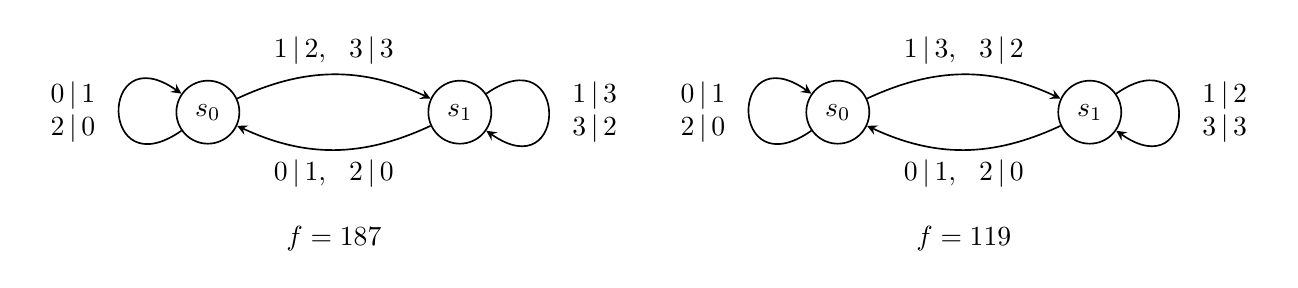
\begin{tikzpicture}[>=stealth,semithick,state/.style={circle,draw,minimum size=8mm,inner sep=0pt}]
\begin{scope}
\node[state] (a0) at (0,0) {$s_0$};
\node[state] (a1) at (3.2,0) {$s_1$};
\draw[->] (a0) to[out=215,in=145,looseness=7] node[left] {$\begin{array}{c}0\,|\,1\\2\,|\,0\end{array}$} (a0);
\draw[->] (a1) to[out=35,in=-35,looseness=7] node[right] {$\begin{array}{c}1\,|\,3\\3\,|\,2\end{array}$} (a1);
\draw[->] (a0) to[bend left=25] node[above] {$1\,|\,2,\ \ 3\,|\,3$} (a1);
\draw[->] (a1) to[bend left=25] node[below] {$0\,|\,1,\ \ 2\,|\,0$} (a0);
\node at (1.6,-1.6) {$f=187$};
\end{scope}
\begin{scope}[xshift=8cm]
\node[state] (b0) at (0,0) {$s_0$};
\node[state] (b1) at (3.2,0) {$s_1$};
\draw[->] (b0) to[out=215,in=145,looseness=7] node[left] {$\begin{array}{c}0\,|\,1\\2\,|\,0\end{array}$} (b0);
\draw[->] (b1) to[out=35,in=-35,looseness=7] node[right] {$\begin{array}{c}1\,|\,2\\3\,|\,3\end{array}$} (b1);
\draw[->] (b0) to[bend left=25] node[above] {$1\,|\,3,\ \ 3\,|\,2$} (b1);
\draw[->] (b1) to[bend left=25] node[below] {$0\,|\,1,\ \ 2\,|\,0$} (b0);
\node at (1.6,-1.6) {$f=119$};
\end{scope}
\end{tikzpicture}
\caption{The Mealy automata defining $s_0$ and $s_1$. An arrow from $s_\nu$ labelled $x\,|\,z$ means that in the state $s_\nu$ the letter $x$ is replaced by $z=\phi_\nu(x)$ (Table~\ref{hr:tab:phi}); the arrow ends at $s_{y(x)}$, the state in which the next letter is read. The letters are the cells $2x+y$, so the arrows into $s_0$ carry the inputs $0,2$ and those into $s_1$ the inputs $1,3$.}
\label{hr:fig:mealy}
\end{figure}

Since the edges of $\Lambda^0_M$ are the two permutations $s_0,s_1$ of the finite level $M+1$, and the inverse of a permutation of a finite set is a positive power of it, $\Lambda^0_M$ is strongly connected if and only if $G$ acts transitively on level $M+1$. Likewise, by Definition~\ref{hr:def:graphs}, a vertex $(\omega,z)$ of $W_M$ is the ordered pair of distinct \emph{siblings} $\bar\omega=u\,\omega_0$ and $u\,z$ of level $M+1$, with common parent $u=\omega_M\cdots\omega_1$ of level $M$, and an edge applies the same generator to both. Hence:

\begin{lemma}\label{hr:lem:Wtree}
$W_M$ is strongly connected if and only if $G$ acts transitively on ordered pairs of distinct siblings of level $M+1$. This holds if $G$ is transitive on level $M$ and, for one vertex $u$ of level $M$, the level-$1$ image of $\{t|_u:t\in G,\ t(u)=u\}$ is $2$-transitive on $\A$.
\end{lemma}

\begin{proof}
The first statement is the remark above. For the second, given ordered sibling pairs $(vx,vz)$ and $(v'x',v'z')$, move $v$ and $v'$ to $u$ by elements of $G$, and then $(x,z)$ to $(x',z')$ by an element of the stabilizer of $u$, which acts on the children of $u$ through its sections at $u$.
\end{proof}

Let $H=\langle s_0^2,s_1\rangle\le G$, and let $x_*=1$ for $f=187$ and $x_*=3$ for $f=119$. Words in $s_0^{\pm1},s_1^{\pm1}$ are composed from right to left.

\begin{lemma}[finite check: section identities]\label{hr:lem:sections}
The following elements of $H$ fix the letter $x_*$ and have the stated sections at $x_*$:
\begin{center}
\begin{tabular}{lll}
\toprule
$f$ & element & section at $x_*$\\
\midrule
$187$, $x_*=1$ & $t_1=s_1s_0^{-2}s_1^2$ & $s_1$\\
& $t_2=s_0^2s_1s_0^{-2}s_1$ & $s_0^2$\\
\midrule
$119$, $x_*=3$ & $t_1=s_1$ & $s_1$\\
& $t_2=s_0^{-2}s_1^3s_0^2$ & $s_0^2s_1$\\
\bottomrule
\end{tabular}
\end{center}
\end{lemma}

\begin{proof}
All four elements are words in $s_0^{\pm2}$ and $s_1^{\pm1}$, so they lie in $H$. By the rules for sections, $s_\nu|_x=s_{y(x)}$, and $s_\nu^{-1}|_x=(s_{y(x')})^{-1}$ with $x'=\phi_\nu^{-1}(x)$. For $f=119$ and $t_1=s_1$: $\phi_1(3)=3$ and $s_1|_3=s_{y(3)}=s_1$. For the other three elements, Table~\ref{hr:tab:sections} follows the letter $x_*$ through the word, from the rightmost generator to the leftmost. Each row gives the generator applied, the letter before and after it (read off from Table~\ref{hr:tab:phi}), and the section of that generator at the letter before it. In each case the last letter is $x_*$. By the product rule, the section of the word at $x_*$ is the product of the sections in the table, taken from the last row on the left to the first row on the right; the last line of each block gives this product and its reduction.
\end{proof}

\begin{table}[ht]
\centering
\small
\begin{tabular}{lcl}
\toprule
\multicolumn{3}{l}{$187$:\quad $t_1=s_1s_0^{-2}s_1^2$}\\
\midrule
step & letter & section\\
\midrule
$s_1$ & $1\mapsto3$ & $s_1$\\
$s_1$ & $3\mapsto2$ & $s_1$\\
$s_0^{-1}$ & $2\mapsto1$ & $s_1^{-1}$\\
$s_0^{-1}$ & $1\mapsto0$ & $s_0^{-1}$\\
$s_1$ & $0\mapsto1$ & $s_0$\\
& & \\
& & \\
\midrule
\multicolumn{3}{l}{$s_0\,s_0^{-1}\,s_1^{-1}\,s_1\,s_1=s_1$}\\
\bottomrule
\end{tabular}
\quad
\begin{tabular}{lcl}
\toprule
\multicolumn{3}{l}{$187$:\quad $t_2=s_0^2s_1s_0^{-2}s_1$}\\
\midrule
step & letter & section\\
\midrule
$s_1$ & $1\mapsto3$ & $s_1$\\
$s_0^{-1}$ & $3\mapsto3$ & $s_1^{-1}$\\
$s_0^{-1}$ & $3\mapsto3$ & $s_1^{-1}$\\
$s_1$ & $3\mapsto2$ & $s_1$\\
$s_0$ & $2\mapsto0$ & $s_0$\\
$s_0$ & $0\mapsto1$ & $s_0$\\
& & \\
\midrule
\multicolumn{3}{l}{$s_0\,s_0\,s_1\,s_1^{-1}\,s_1^{-1}\,s_1=s_0^2$}\\
\bottomrule
\end{tabular}
\quad
\begin{tabular}{lcl}
\toprule
\multicolumn{3}{l}{$119$:\quad $t_2=s_0^{-2}s_1^3s_0^2$}\\
\midrule
step & letter & section\\
\midrule
$s_0$ & $3\mapsto2$ & $s_1$\\
$s_0$ & $2\mapsto0$ & $s_0$\\
$s_1$ & $0\mapsto1$ & $s_0$\\
$s_1$ & $1\mapsto2$ & $s_1$\\
$s_1$ & $2\mapsto0$ & $s_0$\\
$s_0^{-1}$ & $0\mapsto2$ & $s_0^{-1}$\\
$s_0^{-1}$ & $2\mapsto3$ & $s_1^{-1}$\\
\midrule
\multicolumn{3}{l}{$s_1^{-1}s_0^{-1}\,s_0\,s_1\,s_0\,s_0\,s_1=s_0^2s_1$}\\
\bottomrule
\end{tabular}
\caption{Proof of Lemma~\ref{hr:lem:sections}. The generators of each word are applied from right to left, starting at the letter $x_*$ ($x_*=1$ for $187$, $x_*=3$ for $119$). A step $s_\nu$ maps the letter $x$ to $\phi_\nu(x)$ with section $s_{y(x)}$; a step $s_\nu^{-1}$ maps $x$ to $x'=\phi_\nu^{-1}(x)$ with section $s_{y(x')}^{-1}$.}
\label{hr:tab:sections}
\end{table}

\begin{lemma}[finite check: level-$1$ groups]\label{hr:lem:level1}
The level-$1$ image of $H$ is $\langle\phi_0^2,\phi_1\rangle$, which is $\Sym(\A)\cong S_4$ for $187$ and the alternating group $A_4$ for $119$. Both are transitive and $2$-transitive on $\A$.
\end{lemma}

\begin{proof}
The level-$1$ images of $s_0^2$ and $s_1$ are $\phi_0^2$ and $\phi_1$; they are listed in Table~\ref{hr:tab:level1}. For $187$, $\phi_0^2$ is a $3$-cycle and $\phi_1$ a $4$-cycle, so the order of the group they generate is divisible by $12$, and the group contains an odd permutation; so it is $S_4$. For $119$, $\phi_0^2$ and $\phi_1$ are even. Conjugating $\phi_0^2=(0\,3)(1\,2)$ by $\phi_1$ gives $(1\,3)(0\,2)$, and the product of the two is $(0\,1)(2\,3)$, so the group contains the Klein four-group and a $3$-cycle; its order is divisible by $12$, and it is $A_4$. Both $S_4$ and $A_4$ are $2$-transitive on four points: they are transitive, and the stabilizer of a point contains a $3$-cycle, which permutes the other three points cyclically.
\end{proof}

\begin{table}[ht]
\centering
\begin{tabular}{llllll}
\toprule
$f$ & $\phi_0^2$ & $\phi_1$ & orders & signs & $\langle\phi_0^2,\phi_1\rangle$\\
\midrule
$187$ & $(0\,2\,1)$ & $(0\,1\,3\,2)$ & $3$, $4$ & even, odd & $S_4$\\
$119$ & $(0\,3)(1\,2)$ & $(0\,1\,2)$ & $2$, $3$ & even, even & $A_4$\\
\bottomrule
\end{tabular}
\caption{Proof of Lemma~\ref{hr:lem:level1}: the level-$1$ images of the generators $s_0^2$, $s_1$ of $H$, from Table~\ref{hr:tab:phi}.}
\label{hr:tab:level1}
\end{table}

\begin{proposition}\label{hr:prop:tree}
For $f\in\{119,187\}$:
\begin{enumerate}
\item $H$ is self-replicating at $x_*$: for every $t\in H$ there is $t'\in H$ with $t'(x_*)=x_*$ and $t'|_{x_*}=t$; consequently, for every $m\ge0$ and $t\in H$ there is $t'\in H$ with $t'(x_*^m)=x_*^m$ and $t'|_{x_*^m}=t$;
\item $H$, and hence $G$, acts transitively on every level, so $\Lambda^0_M$ is strongly connected for every $M$;
\item $W_M$ is strongly connected for every $M\ge0$.
\end{enumerate}
\end{proposition}

\begin{proof}
(1) On the stabilizer of $x_*$ in $H$, the map $t\mapsto t|_{x_*}$ is a homomorphism, by the product rule for sections. By Lemma~\ref{hr:lem:sections} its image contains $s_1$ and $s_0^2$ (for $119$, $s_0^2=(s_0^2s_1)s_1^{-1}$), hence all of $H$. For $m\ge1$ argue by induction: given $t$, choose $t'\in H$ fixing $x_*$ with $t'|_{x_*}=t$, and $t''\in H$ fixing $x_*^{m}$ with $t''|_{x_*^m}=t'$; then $t''$ fixes $x_*^{m+1}$ and $t''|_{x_*^{m+1}}=t'|_{x_*}=t$. (2) By induction on the level $n$. For $n=1$ this is Lemma~\ref{hr:lem:level1}. Given words $xv$ and $x'v'$ of level $n+1$, choose $t\in H$ with $t(x)=x_*$ and $t'\in H$ with $t'(x')=x_*$, so that the words become $x_*w$ and $x_*w'$; by (1) and the induction hypothesis some element of $H$ fixing $x_*$ has a section mapping $w$ to $w'$. (3) By (2), $G$ is transitive on level $M$. By (1), the sections at $u=x_*^M$ of the elements of $H$ fixing $u$ form all of $H$, whose level-$1$ image is $2$-transitive by Lemma~\ref{hr:lem:level1}. Lemma~\ref{hr:lem:Wtree} applies.
\end{proof}

In the terminology of \cite{Nekrashevych2005}, (1) and (2) say that $H$ is self-replicating and level-transitive. For $119$ the level-$1$ image of $G$ is $S_4$, since $\phi_0$ is a $4$-cycle, while that of $H$ is $A_4$; by Lemma~\ref{hr:lem:level1} the smaller group suffices.

\subsection{The kernel of the offset}\label{hr:sec:kernel}

By Proposition~\ref{hr:prop:tree}(3) and Corollary~\ref{hr:cor:reduce}, $\Aut(X_F)=\langle\sh\rangle\times\ker e$, and every $h\in\ker e$ reads only cells to its right: $h(c)_i=K(c_{[i,i+A]})$ with $A=A(h)$ and $K$ bijective in its first argument. We show $\ker e=\langle F\rangle$. Throughout, $h$, $h_1$, $h_2$ denote elements of $\ker e$ with local rules $K$, $K_1$, $K_2$, and $F^{\pm1}\in\ker e$ by Corollary~\ref{hr:cor:reduce}(1).

\paragraph{Tops.} Let $A=A(h)\ge1$. For $\epsilon=(\epsilon_0,\dots,\epsilon_{A-1})\in\A^A$ let $\vartheta_\epsilon\colon\A\to\A$, $\vartheta_\epsilon(z)=K(\epsilon_0,\dots,\epsilon_{A-1},z)$, be the dependence of $K$ on its last argument when the first $A$ arguments are $\epsilon$. Since $A$ is minimal, some $\vartheta_\epsilon$ is not constant.

\begin{lemma}[diagonal top]\label{hr:lem:top}
Let $A(h)\ge1$. For every $\epsilon\in\A^A$ there are maps $\alpha_\epsilon,\beta_\epsilon\colon\{0,1\}\to\{0,1\}$ with $\vartheta_\epsilon(z)=\bigl(\alpha_\epsilon(x(z)),\,\beta_\epsilon(y(z))\bigr)$.
\end{lemma}

\begin{proof}
Let $c$ have $c_{[1,A]}=\epsilon$, that is $c_{1+j}=\epsilon_j$, and $c_{A+1}=z$; the cell $c_0$ is chosen below. By \eqref{hr:eq:half},
\[
(Fh)(c)_0=\phi_{y(h(c)_1)}\bigl(h(c)_0\bigr)=\phi_{y(\vartheta_\epsilon(z))}\bigl(K(c_0,\epsilon)\bigr).
\]
On the other side, $(hF)(c)_0=K(F(c)_{[0,A]})$, and by (a) the cells $F(c)_j$ with $j<A$ do not involve $z$, while $F(c)_A=\phi_{y(z)}(c_A)$ involves $z$ only through $y(z)$. Since $K$ is bijective in its first argument, we may choose $c_0$ with $y(K(c_0,\epsilon))=1$. Then $\nu\mapsto\phi_\nu(K(c_0,\epsilon))$ is injective by (c), and $hF=Fh$ shows that $y(\vartheta_\epsilon(z))$ is a function of $y(z)$. For the $x$-bit use $hF^{-1}=F^{-1}h$: $(F^{-1}h)(c)_0=\psi_{x(\vartheta_\epsilon(z))}(K(c_0,\epsilon))$, while $(hF^{-1})(c)_0$ involves $z$ only through $x(z)$ by (a); choosing $c_0$ with $x(K(c_0,\epsilon))=1$ and using (c) shows that $x(\vartheta_\epsilon(z))$ is a function of $x(z)$.
\end{proof}

Put $\mathcal X_h=\{\epsilon:\alpha_\epsilon\text{ is not constant}\}$ and $\mathcal Y_h=\{\epsilon:\beta_\epsilon\text{ is not constant}\}$. By minimality of $A$, $\mathcal X_h\cup\mathcal Y_h\ne\emptyset$. Call $h$ of \emph{$y$-type} if $\mathcal Y_h\ne\emptyset=\mathcal X_h$, of \emph{$x$-type} if $\mathcal X_h\ne\emptyset=\mathcal Y_h$, and of \emph{both types} if both are nonempty. A nonconstant map $\{0,1\}\to\{0,1\}$ is a bijection. By \eqref{hr:eq:half}, $F$ has anticipation $1$ and $\vartheta_\epsilon(z)=\phi_{y(z)}(\epsilon_0)$, whose $x$-bit $y(\epsilon_0)$ is constant; so $F$ is of $y$-type, with $\mathcal Y_F=\{\epsilon_0:y(\epsilon_0)=1\}$ by (c). Likewise $F^{-1}$ is of $x$-type with anticipation $1$.

\begin{lemma}\label{hr:lem:FF}
\begin{enumerate}
\item If $h$ is of $x$-type, then $A(hF)\le A(h)$, and if equality holds, $hF$ is of $y$-type.
\item If $h$ is of $y$-type, then $A(hF^{-1})\le A(h)$, and if equality holds, $hF^{-1}$ is of $x$-type.
\end{enumerate}
\end{lemma}

\begin{proof}
(1) Let $A=A(h)$. $(hF)(c)_0=K(F(c)_{[0,A]})$, and since $h$ is of $x$-type, $K$ reads its last argument $F(c)_A$ only through $x(F(c)_A)=y(c_A)$, by (b). The cells $F(c)_j$, $j<A$, read $c_{[0,A]}$, and $c_A$ only through $y(c_A)$ (in $F(c)_{A-1}=\phi_{y(c_A)}(c_{A-1})$). So $(hF)(c)_0$ depends only on $c_{[0,A]}$, and on $c_A$ only through $y(c_A)$. If $A(hF)=A$, its tops therefore do not depend on $x(z)$, so by Lemma~\ref{hr:lem:top} every $\alpha_\epsilon$ is constant, and $hF$ is of $y$-type. (2) is the mirror argument: $K$ reads $F^{-1}(d)_A$ only through $y(F^{-1}(d)_A)=x(d_A)$, and $F^{-1}(d)_{A-1}=\psi_{x(d_A)}(d_{A-1})$.
\end{proof}

\begin{lemma}\label{hr:lem:comp}
Let $A(h_1),A(h_2)\ge1$.
\begin{enumerate}
\item If $\mathcal Y_{h_1}$ and $\mathcal Y_{h_2}$ are nonempty, then $A(h_1h_2)=A(h_1)+A(h_2)$ and $\mathcal Y_{h_1h_2}\ne\emptyset$; if $h_1$ and $h_2$ are of $y$-type, so is $h_1h_2$.
\item The same holds with $\mathcal X$ in place of $\mathcal Y$ and $x$-type in place of $y$-type.
\end{enumerate}
\end{lemma}

\begin{proof}
Write $A_j=A(h_j)$ and $A=A_1+A_2$. $(h_1h_2)(c)_0=K_1(h_2(c)_{[0,A_1]})$ reads only $c_{[0,A]}$, and of the cells $h_2(c)_j$, $0\le j\le A_1$, only $h_2(c)_{A_1}=K_2(c_{[A_1,A]})$ involves $c_A$. Fix $c_{[0,A)}$ and let $z=c_A$ vary. Then $h_2(c)_{[0,A_1)}=\epsilon'$ is fixed, $h_2(c)_{A_1}=\vartheta^{(2)}_{\epsilon''}(z)$ with $\epsilon''=c_{[A_1,A)}$, and the top of $h_1h_2$ at $c_{[0,A)}$ is $\vartheta^{(1)}_{\epsilon'}\circ\vartheta^{(2)}_{\epsilon''}$, whose $x$-part is $\alpha^{(1)}_{\epsilon'}\circ\alpha^{(2)}_{\epsilon''}$ and whose $y$-part is $\beta^{(1)}_{\epsilon'}\circ\beta^{(2)}_{\epsilon''}$, by Lemma~\ref{hr:lem:top}. Choose $\epsilon''\in\mathcal Y_{h_2}$. As $c_{[0,A_1)}$ varies with $c_{[A_1,A)}=\epsilon''$ fixed, $h_2(c)_{[0,A_1)}$ takes every value in $\A^{A_1}$: solve for $c_{A_1-1},c_{A_1-2},\dots,c_0$ in turn, using that $K_2$ is bijective in its first argument. So we may choose $\epsilon'\in\mathcal Y_{h_1}$. Then the $y$-part of the top is a composite of two bijections, so $h_1h_2$ depends on $c_A$, $A(h_1h_2)=A$, and $\mathcal Y_{h_1h_2}\ne\emptyset$. If both are of $y$-type, every $\alpha^{(j)}$ is constant, so every $x$-part of a top of $h_1h_2$ is constant and $h_1h_2$ is of $y$-type. (2) is identical.
\end{proof}

By Lemma~\ref{hr:lem:comp} and induction, $F^b$ is of $y$-type with $A(F^b)=b$ and $F^{-b}$ is of $x$-type with $A(F^{-b})=b$, for $b\ge1$. In particular $F$ has infinite order.

\begin{lemma}[no both-type]\label{hr:lem:both}
No $h\in\ker e$ is of both types. Hence every $h\in\ker e$ with $A(h)\ge1$ is of $x$-type or of $y$-type.
\end{lemma}

\begin{proof}
Suppose $h$ is of both types, so $A(h)\ge1$. If $A(h^{-1})=0$, then $h^{-1}$ is a cellwise permutation commuting with $F$, so $h^{-1}=\mathrm{id}$ by Lemma~\ref{hr:lem:P}, contradicting $A(h)\ge1$. Otherwise $\mathcal X_{h^{-1}}$ or $\mathcal Y_{h^{-1}}$ is nonempty, and Lemma~\ref{hr:lem:comp}, applied to $h_1=h$ and $h_2=h^{-1}$ with $\mathcal X$ or $\mathcal Y$ accordingly, gives $A(\mathrm{id})=A(h)+A(h^{-1})\ge2$, whereas $A(\mathrm{id})=0$.
\end{proof}

\begin{lemma}[no half step]\label{hr:lem:half}
There is no $h\in\ker e$ of $y$-type with $A(h)=A\ge1$ such that $h'=hF^{-1}$ is of $x$-type with $A(h')=A$.
\end{lemma}

\begin{proof}
Suppose there is. By Lemma~\ref{hr:lem:comp}, $h^2$ is of $y$-type with $A(h^2)=2A$, and $h'^2=h^2F^{-2}$ is of $x$-type with $A(h'^2)=2A$. Let $\hat h=h^2F^{-1}=h'^2F$. Lemma~\ref{hr:lem:FF}(2) applied to $h^2$ gives $A(\hat h)\le2A$, with $\hat h$ of $x$-type in case of equality; Lemma~\ref{hr:lem:FF}(1) applied to $h'^2$ gives $\hat h$ of $y$-type in case of equality. A map is not of both $x$-type and $y$-type, so $A(\hat h)\le2A-1$. We consider the three possibilities left by Lemma~\ref{hr:lem:both}.
\begin{itemize}
\item $A(\hat h)=0$. Then $\hat h$ is a cellwise permutation commuting with $F$, so $\hat h=\mathrm{id}$ by Lemma~\ref{hr:lem:P}, and $h^2=F$. But $A(F)=1<2\le2A=A(h^2)$.
\item $\hat h$ is of $y$-type. By Lemma~\ref{hr:lem:FF}(2), $A(h'^2)=A(\hat hF^{-1})\le A(\hat h)<2A$, a contradiction.
\item $\hat h$ is of $x$-type. By Lemma~\ref{hr:lem:FF}(1), $A(h^2)=A(\hat hF)\le A(\hat h)<2A$, a contradiction.\qedhere
\end{itemize}
\end{proof}

\begin{theorem}\label{hr:thm:kernel}
For $f\in\{119,187\}$, $\ker e=\langle F\rangle$, and $A(F^b)=|b|$.
\end{theorem}

\begin{proof}
We show by strong induction on $A=A(h)$ that every $h\in\ker e$ is a power of $F$. If $A=0$, then $h=\mathrm{id}$ by Lemma~\ref{hr:lem:P}. Let $A\ge1$; by Lemma~\ref{hr:lem:both}, $h$ is of $y$-type or of $x$-type.

\emph{$h$ of $y$-type.} Let $h'=hF^{-1}\in\ker e$. By Lemma~\ref{hr:lem:FF}(2), $A(h')\le A$, and if $A(h')=A$ then $h'$ is of $x$-type, which Lemma~\ref{hr:lem:half} excludes. So $A(h')<A$, by induction $h'=F^{b'}$, and $h=F^{b'+1}$.

\emph{$h$ of $x$-type.} Let $h''=hF\in\ker e$. By Lemma~\ref{hr:lem:FF}(1), $A(h'')\le A$, and if $A(h'')=A$ then $h''$ is of $y$-type with $h''F^{-1}=h$ of $x$-type and the same anticipation, which Lemma~\ref{hr:lem:half}, applied to $h''$, excludes. So $A(h'')<A$, $h''=F^{b''}$ by induction, and $h=F^{b''-1}$.

The formula $A(F^b)=|b|$ is the statement following Lemma~\ref{hr:lem:comp}.
\end{proof}

\begin{proof}[Proof of Theorem~\ref{hr:thm:main}]
By the conjugacies of Section~\ref{hr:sec:setting} it suffices to take $f\in\{119,187\}$. By Proposition~\ref{hr:prop:tree}(3), $W_M$ is strongly connected for every $M$, so Corollary~\ref{hr:cor:reduce} gives $\Aut(X_F)=\langle\sh\rangle\times\ker e$, and $\ker e=\langle F\rangle$ by Theorem~\ref{hr:thm:kernel}. If $\sh^aF^b=\mathrm{id}$, then $a=-e(\sh^aF^b)=0$ and $F^b=\mathrm{id}$, so $b=0$ since $A(F^b)=|b|$. Lemma~\ref{lem:spacetime} translates this into a statement about the automorphism group of the spacetime subshift.
\end{proof}

\subsection{One-sided automorphisms}\label{hr:sec:onesided}

The elements of $\ker e$ and their inverses read only cells to their right. Such maps are the automorphisms of the one-sided full shift, and Theorem~\ref{hr:thm:kernel} can be stated in these terms.

\begin{definition}\label{hr:def:onesided}
A block map $h$ of $\A^{\Z}$ is \emph{right-sided} if there are $A\ge0$ and $K\colon\A^{A+1}\to\A$ with $h(c)_i=K(c_i,\dots,c_{i+A})$ for all $c$ and $i$. A \emph{one-sided automorphism} of $\A^{\Z}$ is an invertible block map $h$ such that both $h$ and $h^{-1}$ are right-sided.
\end{definition}

A composite of right-sided block maps is right-sided, so the one-sided automorphisms form a subgroup of $\Aut(\A^{\Z})$. The shift $\sh$ is right-sided, but $\sh^{-1}$ is not, so $\sh$ is not a one-sided automorphism. Let $\mathbb N=\{0,1,2,\dots\}$, let $\sh_+$ be the shift on $\A^{\mathbb N}$, $\sh_+(c)_i=c_{i+1}$, and let $\Aut(\A^{\mathbb N})$ be the group of homeomorphisms of $\A^{\mathbb N}$ commuting with $\sh_+$; the automorphism groups of one-sided shifts of finite type are studied in \cite{BFK1990}. A right-sided block map $h$ with local rule $K$ defines a continuous map $h_+\colon\A^{\mathbb N}\to\A^{\mathbb N}$, $h_+(c)_i=K(c_i,\dots,c_{i+A})$, which commutes with $\sh_+$ and satisfies
\begin{equation}\label{hr:eq:restrict}
h_+\bigl(c|_{\mathbb N}\bigr)=h(c)|_{\mathbb N}\qquad(c\in\A^{\Z}).
\end{equation}

\begin{lemma}\label{hr:lem:onesided}
\begin{enumerate}
\item If $h$ and $h'$ are right-sided block maps, then $(hh')_+=h_+h'_+$, and $h_+=h'_+$ implies $h=h'$.
\item The map $h\mapsto h_+$ is an isomorphism from the group of one-sided automorphisms of $\A^{\Z}$ onto $\Aut(\A^{\mathbb N})$.
\item If $h$ is a one-sided automorphism and $h(c)_i=K(c_i,\dots,c_{i+A})$, then $K$ is a bijection in its first argument when the others are fixed.
\end{enumerate}
\end{lemma}

\begin{proof}
(1) Every element of $\A^{\mathbb N}$ is $c|_{\mathbb N}$ for some $c\in\A^{\Z}$, and by \eqref{hr:eq:restrict}, applied to $h'$, to $h$ and to $hh'$,
\[
h_+\bigl(h'_+(c|_{\mathbb N})\bigr)=h_+\bigl(h'(c)|_{\mathbb N}\bigr)=h(h'(c))|_{\mathbb N}=(hh')_+\bigl(c|_{\mathbb N}\bigr).
\]
If $h_+=h'_+$, then for every $c\in\A^{\Z}$ and $i\in\Z$, since $h$ and $h'$ commute with $\sh$,
\[
h(c)_i=h(\sh^ic)_0=h_+\bigl((\sh^ic)|_{\mathbb N}\bigr)_0=h'_+\bigl((\sh^ic)|_{\mathbb N}\bigr)_0=h'(c)_i.
\]

(2) Let $h$ be a one-sided automorphism. By (1), $h_+(h^{-1})_+=(h^{-1})_+h_+=\mathrm{id}_+$, and $\mathrm{id}_+$ is the identity of $\A^{\mathbb N}$. So $h_+$ is a continuous bijection of the compact space $\A^{\mathbb N}$ commuting with $\sh_+$, that is, $h_+\in\Aut(\A^{\mathbb N})$, and $h\mapsto h_+$ is an injective homomorphism by (1). To see that it is surjective, let $\chi\in\Aut(\A^{\mathbb N})$. The map $c\mapsto\chi(c)_0$ is continuous on the compact space $\A^{\mathbb N}$, so it depends only on $c_0,\dots,c_A$ for some $A$, say $\chi(c)_0=K(c_0,\dots,c_A)$; then $\chi(c)_i=\chi(\sh_+^ic)_0=K(c_i,\dots,c_{i+A})$. In the same way $\chi^{-1}(c)_i=K'(c_i,\dots,c_{i+A'})$. Let $h$ and $h'$ be the right-sided block maps of $\A^{\Z}$ with local rules $K$ and $K'$, so that $h_+=\chi$ and $h'_+=\chi^{-1}$. By (1), $(hh')_+=(h'h)_+=\mathrm{id}_+$, and hence $hh'=h'h=\mathrm{id}$. So $h$ is a one-sided automorphism with $h_+=\chi$.

(3) Let $c$ and $c'$ differ only at the site $i$, and suppose that $h(c)_i=h(c')_i$. For $j>i$ the cells $h(c)_j$ and $h(c')_j$ are read from sites $\ge j>i$, where $c=c'$. So $hc$ and $hc'$ agree at every site $\ge i$, and since $h^{-1}$ is right-sided, $c_i=h^{-1}(hc)_i=h^{-1}(hc')_i=c'_i$, a contradiction. Hence $K$ is injective, so bijective, in its first argument.
\end{proof}

By \eqref{hr:eq:half}, $F$ and $F^{-1}$ are right-sided, for every rule of the form $f(a,b,c)=g(b,c)$. So $F$ is a one-sided automorphism, and $F_+$, given by $F_+(c)_i=\phi_{y(c_{i+1})}(c_i)$ for $i\ge0$, is an automorphism of the one-sided full shift on four letters.

\begin{corollary}\label{hr:cor:onesided}
Let $f\in\{119,187\}$ and $F=F_f$.
\begin{enumerate}
\item The one-sided automorphisms of $\A^{\Z}$ that commute with $F$ are exactly the elements of $\ker e$, that is, the powers of $F$.
\item $F_+$ has infinite order, and its centralizer in $\Aut(\A^{\mathbb N})$ is $\langle F_+\rangle\cong\Z$.
\end{enumerate}
\end{corollary}

\begin{proof}
(1) The elements of $\ker e$ are one-sided automorphisms by Corollary~\ref{hr:cor:reduce}(2), they commute with $F$, and $\ker e=\langle F\rangle$ by Theorem~\ref{hr:thm:kernel}. Conversely, let $h$ be a one-sided automorphism commuting with $F$. Then $h\in\Aut(X_F)$, and $e(h)$ is defined by Propositions~\ref{hr:prop:tree}(3) and~\ref{hr:prop:offset}. Let $Q=(c,c')$ be a pair with right edge $p$. For $i>p$ the cells $h(c)_i$ and $h(c')_i$ are read from sites $\ge i>p$, where $c=c'$, so $\lambda(hQ)\le p$. Hence $e(h)\le0$. The same applies to $h^{-1}$, so $-e(h)=e(h^{-1})\le0$ by Corollary~\ref{hr:cor:reduce}(1). So $e(h)=0$.

(2) By Lemma~\ref{hr:lem:onesided}(2), $F_+^b=(F^b)_+$ for $b\in\Z$, and $F_+^b=\mathrm{id}$ only if $F^b=\mathrm{id}$, that is, only if $b=0$, since $A(F^b)=|b|$ by Theorem~\ref{hr:thm:kernel}. Let $\chi\in\Aut(\A^{\mathbb N})$ commute with $F_+$. By Lemma~\ref{hr:lem:onesided}(2), $\chi=h_+$ for a one-sided automorphism $h$, and $(hF)_+=\chi F_+=F_+\chi=(Fh)_+$, so $hF=Fh$ by Lemma~\ref{hr:lem:onesided}(1). By (1), $h=F^b$ for some $b$, and $\chi=F_+^b$.
\end{proof}

Since $\kappa$ is a cellwise map, conjugation by $\kappa_+$ carries Corollary~\ref{hr:cor:onesided} over to the rules $238$ and $221$. For the four reflected rules $63$, $252$, $243$ and $207$ it holds with $\A^{\mathbb N}$ replaced by $\A^{-\mathbb N}$ and right-sided maps by left-sided ones.

\begin{remark}[what the kernel argument uses]\label{hr:rem:general}
For the rules of Theorem~\ref{hr:thm:main}, Section~\ref{hr:sec:kernel} uses the following about $\ker e$ and nothing else: it is a group containing $F$, all of whose elements commute with $F$; each of its elements is right-sided, with a local rule that is bijective in its first argument; the facts (a) and (b); from (c), only that $\nu\mapsto\phi_\nu(z)$ is injective for the cells $z$ with $y(z)=1$ and $\nu\mapsto\psi_\nu(z)$ for the cells with $x(z)=1$; and Lemma~\ref{hr:lem:P}. No window graph enters. The group of one-sided automorphisms commuting with $F$ has these properties by Lemma~\ref{hr:lem:onesided}, so Corollary~\ref{hr:cor:onesided}(1) can also be proved without the window graphs, by applying Section~\ref{hr:sec:kernel} to that group. The condition that $h^{-1}$ is right-sided cannot be dropped there: $\sh$ is right-sided and commutes with $F$, and it is not a power of $F$. We make no claim for other rules that ignore their left argument. When a nontrivial cellwise permutation commutes with $F$, as $\kappa$ does for rule $102=b\oplus c$, the proofs of Lemmas~\ref{hr:lem:both} and~\ref{hr:lem:half} do not apply.
\end{remark}

\begin{remark}[automorphisms of small radius]\label{hr:rem:census}
Let $f\in\{119,187\}$. By Theorem~\ref{hr:thm:kernel} and Corollary~\ref{hr:cor:reduce}(2), $F^b(c)_i$ is a function of the cells $c_i,\dots,c_{i+|b|}$ that is bijective in $c_i$ and, for $b\ne0$, not independent of $c_{i+|b|}$. So $\sh^aF^b(c)_i$ depends on both ends of the interval $[i+a,\,i+a+|b|]$ and on no cell outside it, and the least radius of $\sh^aF^b$ is $\max(|a|,|a+|b||)$, which can be smaller than $|a|+|b|$. The pairs $(a,b)$ with $[a,a+|b|]\subset[-R,R]$ are those with $-R\le a\le R$ and $|b|\le R-a$, and there are $\sum_{a=-R}^{R}(2(R-a)+1)=(2R+1)^2$ of them. So $X_F$ has exactly $(2R+1)^2$ automorphisms of radius at most $R$; by the conjugacies of Section~\ref{hr:sec:setting} the same count holds for all eight rules of Theorem~\ref{hr:thm:main} (for $63$, which reads $(a,b)$, the interval is $[a-|b|,a]$). For $R=1,2,3$ this gives $9$, $25$ and $49$ automorphisms, and these are exactly the invertible maps in the exhaustive enumeration of the block maps of radius at most $3$ commuting with $F$ in \cite{PaperD}. This enumeration and the other computations that confirm Theorem~\ref{hr:thm:main} are described in Appendix~\ref{app:confirm}; none of them is used in a proof.
\end{remark}


\appendix
\section{Computations}\label{app:comp}

This appendix specifies the finite computations of the paper. Every result marked as computer-assisted in the text is the output of a terminating exact search over a finite set. Section~\ref{app:method} describes the enumeration of commuting block maps, Section~\ref{app:proofs} the computations on which computer-assisted propositions rely, Section~\ref{app:stated} the computations whose results are stated in remarks, and Section~\ref{app:confirm} computations that confirm results proved by hand. The programs accompany the paper as supplementary material, in its directory \texttt{code/}; the file \texttt{README.md} there states, for each program, what it computes and its expected output.

\subsection{Enumeration of commuting block maps}\label{app:method}

\emph{Commutation as a finite constraint.} Let $h$ be a block map of radius $R$ with local rule $h_{\mathrm{loc}}$, and $F=F_f$ with $f$ elementary. Both $h\circ F$ and $F\circ h$ are block maps of radius $R+1$, so they are equal if and only if their local rules agree on every word $w\in\A^{2R+3}$. Write $n=2R+1$ and, for $w=(w_0,\dots,w_{2R+2})$, let $v_1,v_2,v_3$ be the three subwords of length $n$ starting at positions $0,1,2$, and let $v_F$ be the word of length $n$ obtained by applying the local rule of $F$ to $w$. Then
\[
(h\circ F)(w)=h_{\mathrm{loc}}(v_F),\qquad (F\circ h)(w)=\Bigl(h_{\mathrm{loc}}(v_2)_y,\ h_{\mathrm{loc}}(v_2)_x\oplus f\bigl(h_{\mathrm{loc}}(v_1)_y,h_{\mathrm{loc}}(v_2)_y,h_{\mathrm{loc}}(v_3)_y\bigr)\Bigr),
\]
where the subscripts $x,y$ denote the two output bits. Writing $X_v,Y_v$ for the two unknown bits of the table entry $h_{\mathrm{loc}}(v)$, each word $w$ contributes the two constraints
\begin{equation}\label{app:eq:constraints}
X_{v_F}=Y_{v_2},\qquad Y_{v_F}\oplus X_{v_2}=f(Y_{v_1},Y_{v_2},Y_{v_3}).
\end{equation}
The first is two binary clauses; the second is a constraint on at most five variables, encoded by its truth table in at most sixteen clauses. Altogether there are $2\cdot4^{2R+1}$ variables and at most $18\cdot4^{2R+3}$ clauses. For an automaton of radius $r$ of the form \eqref{gen:eq:F} the same encoding is used with words of length $2R+2r+1$ and the $2r+1$ subwords of length $n$ that $f$ reads.

\emph{Enumeration and verification.} All solutions are enumerated by repeated solving with blocking clauses, using PySAT \cite{PySAT} with CaDiCaL \cite{CaDiCaL} or MiniSat \cite{MiniSat}. Every table returned by the solver is re-checked, independently of the clauses, by evaluating $h\circ F$ and $F\circ h$ on all words. Each solution is then matched against the maps $\sh^aF^b$ of radius at most $R$, which are built directly by composing local rules, and against the constant maps. The enumeration asserts that every $\sh^aF^b$ of radius at most $R$ occurs among the solutions, which checks the encoding against the maps known in advance to commute.

\emph{Invertibility.} A block map is an automorphism of $\A^{\Z}$ if and only if it is injective. Injectivity of a block map of radius $R$ is decided exactly by the pair graph: its vertices are the pairs $(u,v)$ of words of length $2R$, with an edge $(u,v)\to(u',v')$ labelled $(a,b)\in\A^2$ whenever $u'$ and $v'$ are $ua$ and $vb$ with their first letters removed, and $h_{\mathrm{loc}}(ua)=h_{\mathrm{loc}}(vb)$. Then $h$ fails to be injective if and only if a bi-infinite path passes through an off-diagonal vertex, which is decided by iteratively deleting vertices without a predecessor or without a successor. Where only the invertible commuting maps are wanted, balance is added to the clauses: a surjective block map of radius $R$ is balanced \cite{Hedlund1969}, each output symbol occurring exactly $4^{2R}$ times in its table, so the balanced commuting maps are enumerated and each is submitted to the pair-graph test. The supplementary material contains \texttt{sat/centralizer.py} for the elementary rules, \texttt{sat/cent\_r.py} for the automata \eqref{gen:eq:F} of radius $r$, and \texttt{sat/invertible\_sat.py} for the enumeration with balance.

\subsection{Computations used in computer-assisted propositions}\label{app:proofs}

\emph{The certificate $(\mathrm T_P)$.}\label{app:general} For given $r$, $g$ and $P$, the sets $\mathrm{Im}_m$ of Section~\ref{gen:sec:tower} are computed by iterating the successor relation on the $2^{2rP}$ column states until they stabilise at $S_\infty$, and $(\mathrm T_P)$ is then tested. Increasing $P$ gives a semi-decision procedure for a sufficient condition; we do not claim that \textup{($\Lambda$)} implies $(\mathrm T_P)$ for some $P$.

\emph{Proposition~\ref{gen:prop:r2TP}.} For each of the $65\,536$ functions $g$ of four variables, $(\mathrm T_P)$ is tested for $P=1,2,3,4$ in turn, up to the least $P$ for which it holds. The supplementary material contains two independent programs for this, which represent the column states differently (\texttt{scan\_r2.py} with \texttt{scan\_r2b.py}, and \texttt{tp\_direct.py}), and a third (\texttt{compare.py}) that compares their tables of least $P$ for every $g$; the tables are identical. The program \texttt{scan\_r2.py} also builds $\Lambda_2$ and $\Lambda_3$ from the cell rule for the functions with no $(\mathrm T_P)$, $P\le3$: for the $44$ functions with least $P=4$ the graphs $\Lambda_2$ and $\Lambda_3$ are strongly connected, and for $g=\xi_3$ and $g=1\oplus\xi_3$ the graph $\Lambda_3$ is not. For $g=\xi_3$ the graphs $\Lambda_M$, $2\le M\le5$, are built in the same way and are not strongly connected. The program \texttt{xcheck.py} compares the two $(\mathrm T_P)$ routines on $153$ functions and counts the functions that satisfy \textup{(N)} and \textup{(D)}.

\emph{Tables~\ref{gen:tab:r2}, \ref{gen:tab:r2ten} and~\ref{gen:tab:r3}, and Propositions~\ref{gen:prop:r2} and~\ref{gen:prop:r3}.} $J(g)$ and self-duality are computed from the truth table. $(\mathrm T_P)$ is tested for $P\le4$ at radius $2$ and $P\le3$ at radius $3$. Condition $(\mathrm I)_q$ is tested by enumerating, for each $n$, the points of least spatial period $n$, computing the stabiliser of each $\Z^2$-orbit, and counting the orbits with each stabiliser; this gives $k(\mathcal L)$ exactly (Lemma~\ref{gen:lem:stab}). The witness listed is the first in the order of increasing $n$, then increasing index $nb$, then increasing $s$; the enumeration goes up to $n=5$. Each of these quantities is computed by two independent programs, with identical results; the supplementary material contains \texttt{examples.py} and \texttt{checks3.py}. In addition, $\Lambda_M$ built from the cell rule is strongly connected for $M\le3$ for every rule of Tables~\ref{gen:tab:r2} and~\ref{gen:tab:r2ten}, and for $M\le2$ for every rule of Table~\ref{gen:tab:r3}. The column ``strip'' of Table~\ref{gen:tab:r2} is a SAT encoding of \eqref{gen:eq:star}, as a system of constraints on the truth table of $\gamma$, whose enumeration stops after $20$ solutions (\texttt{sat/strip.py}); the column ``extra'' is the enumeration of Section~\ref{app:method} (\texttt{sat/cent\_r.py}). The statements about rules $90$ and $150$ in Section~\ref{gen:sec:examples} are computed in the same way.

\subsection{Computer-assisted statements in remarks}\label{app:stated}

\emph{Affine rules} (Remark~\ref{pm:rem:linear}). $\Lambda_M$ and the eventual image of $\Gamma_{w,0}$ are built directly from the local rule and tested for strong connectivity. For rule $90$ the graph $\Lambda_M$ is not strongly connected for $1\le M\le8$; this is the range quoted in Remark~\ref{pm:rem:linear} and in Section~\ref{gen:sec:examples}.

\subsection{Confirmations of results proved by hand}\label{app:confirm}

The following computations confirm results that the paper proves by hand. None of them is used in a proof.

\emph{Rule $30$ at radius at most $4$} (Theorem~\ref{thm:rigidity30}). The enumeration of Section~\ref{app:method} for $f=30$ and $R=1,2,3,4$ gives exactly $2R^2+2R+3$ tables, that is $7$, $15$, $27$ and $43$: the $2R^2+2R+1$ tables of the maps $\sh^aF_{30}^b$ with $|a|+|b|\le R$, which are pairwise distinct and invertible, and the two constant maps onto $(0,0)^{\Z}$ and $(1,1)^{\Z}$. So $\Cent_4(F_{30})$ consists of the elements of $\langle\sh,F_{30}\rangle$ of radius at most $4$ and these two constants, in agreement with Theorem~\ref{thm:rigidity30}; this also determines the non-invertible commuting block maps of radius at most $4$, which the theorem does not address. The enumeration is part of \cite{PaperD}.

\emph{The elementary permutive rules} (Theorem~\ref{pm:thm:main}). For $f=45,75,135$ and $R=1$, and for $f=45,135$ and $R=2$, the enumeration gives only the maps $\sh^aF^b$ and constant maps. For the eight non-affine left-permutive rules, $\Lambda_M$ built from the cell rule is strongly connected for $M\le5$.

\emph{Rules that read two neighbours} (Section~\ref{sec:halfradius}). The three finite checks, Lemmas~\ref{hr:lem:P}, \ref{hr:lem:sections} and~\ref{hr:lem:level1}, are confirmed by direct computation (\texttt{halfradius/hr\_checks.py}): the section identities by free reduction of the section words and by evaluating both sides on all words of length $7$. The window graph $W_M$, built from the cell rule, is strongly connected for $M\le6$, and the level-$1$ image of $\{t|_{x_*^M}:t\in G,\ t(x_*^M)=x_*^M\}$ is exactly $A_4$ for $119$ when $1\le M\le10$ (and $S_4$ for $M=0$), and $S_4$ for $187$ when $0\le M\le10$. An exhaustive SAT enumeration (\texttt{halfradius/kernel\_sat.py}) of the right-sided block maps of anticipation at most $6$ that commute with $F$ and are bijective in their first argument, as every right-sided automorphism with right-sided inverse is (Lemma~\ref{hr:lem:onesided}(3)), gives exactly the powers $F^b$ with $|b|\le6$, for both $119$ and $187$. For rule $102$ the same enumeration gives non-invertible right-sided block maps commuting with $F$. The enumeration of \cite{PaperD} gives, for the classes of $63$ and $187$, exactly the $(2R+1)^2$ automorphisms $\sh^aF^b$ of radius at most $R$ for $R\le3$ (Remark~\ref{hr:rem:census}).



\medskip
\noindent\textbf{Use of AI tools.} Large language models (Anthropic's Claude models) were used extensively in this work: to propose and develop proofs, to design, write and run the computer searches and their independent re-implementations, to check proofs and computations, and to draft the manuscript. The models are not authors. The author has reviewed the content and takes full responsibility for it. All code and computational output accompany the paper (Appendix~\ref{app:comp}).

\begin{thebibliography}{99}

\bibitem{BRY2018} M.~Baake, J.~A.~G.~Roberts and R.~Yassawi, Reversing and extended symmetries of shift spaces, \emph{Discrete Contin. Dyn. Syst.} \textbf{38} (2018), 835--866.

\bibitem{CaDiCaL} A.~Biere, K.~Fazekas, M.~Fleury and M.~Heisinger, CaDiCaL, Kissat, Paracooba, Plingeling and Treengeling entering the SAT Competition 2020, in \emph{Proc. SAT Competition 2020}, Univ. Helsinki, 2020, 51--53.

\bibitem{BFK1990} M.~Boyle, J.~Franks and B.~Kitchens, Automorphisms of one-sided subshifts of finite type, \emph{Ergodic Theory Dynam. Systems} \textbf{10} (1990), 421--449.

\bibitem{BoyleLind1997} M.~Boyle and D.~Lind, Expansive subdynamics, \emph{Trans. Amer. Math. Soc.} \textbf{349} (1997), 55--102.

\bibitem{BLR1988} M.~Boyle, D.~Lind and D.~Rudolph, The automorphism group of a shift of finite type, \emph{Trans. Amer. Math. Soc.} \textbf{306} (1988), 71--114.

\bibitem{CHR1979} E.~M.~Coven, G.~A.~Hedlund and F.~Rhodes, The commuting block maps problem, \emph{Trans. Amer. Math. Soc.} \textbf{249} (1979), 113--138.

\bibitem{CFK2019} V.~Cyr, J.~Franks and B.~Kra, The spacetime of a shift endomorphism, \emph{Trans. Amer. Math. Soc.} \textbf{371} (2019), 461--488.

\bibitem{CK2015} V.~Cyr and B.~Kra, The automorphism group of a shift of linear growth: beyond transitivity, \emph{Forum Math. Sigma} \textbf{3} (2015), e5.

\bibitem{PaperA} M.~Dayah, Reversible rule 110 has no hidden symmetries: six families of second-order cellular automata settled by edge moves, in preparation.

\bibitem{PaperBsupp} M.~Dayah, The two-copy window graph of a permutive second-order cellular automaton, supplement to this paper.

\bibitem{PaperC} M.~Dayah, Every finite group from a wall: large automorphism groups of second-order cellular automata, in preparation.

\bibitem{PaperD} M.~Dayah, The 88 second-order elementary cellular automata: a classification by automorphism group, in preparation.

\bibitem{DDMP2016} S.~Donoso, F.~Durand, A.~Maass and S.~Petite, On automorphism groups of low complexity subshifts, \emph{Ergodic Theory Dynam. Systems} \textbf{36} (2016), 64--95.

\bibitem{MiniSat} N.~E\'en and N.~S\"orensson, An extensible SAT-solver, in \emph{Theory and Applications of Satisfiability Testing (SAT 2003)}, Lecture Notes in Comput. Sci. 2919, Springer, 2004, 502--518.

\bibitem{Hedlund1969} G.~A.~Hedlund, Endomorphisms and automorphisms of the shift dynamical system, \emph{Math. Systems Theory} \textbf{3} (1969), 320--375.

\bibitem{Hochman2010} M.~Hochman, On the automorphism groups of multidimensional shifts of finite type, \emph{Ergodic Theory Dynam. Systems} \textbf{30} (2010), 809--840.

\bibitem{PySAT} A.~Ignatiev, A.~Morgado and J.~Marques-Silva, PySAT: a Python toolkit for prototyping with SAT oracles, in \emph{Theory and Applications of Satisfiability Testing (SAT 2018)}, Lecture Notes in Comput. Sci. 10929, Springer, 2018, 428--437.

\bibitem{KimRoush1990} K.~H.~Kim and F.~W.~Roush, On the automorphism groups of subshifts, \emph{Pure Math. Appl. Ser. B} \textbf{1} (1990), no.~4, 203--230.

\bibitem{Kopra2022} J.~Kopra, Glider automata on all transitive sofic shifts, \emph{Ergodic Theory Dynam. Systems} \textbf{42} (2022), 3716--3744.

\bibitem{Ledrappier1978} F.~Ledrappier, Un champ markovien peut \^etre d'entropie nulle et m\'elangeant, \emph{C. R. Acad. Sci. Paris S\'er. A-B} \textbf{287} (1978), A561--A563.

\bibitem{MooreBoykett1997} C.~Moore and T.~Boykett, Commuting cellular automata, \emph{Complex Systems} \textbf{11} (1997), 55--64.

\bibitem{Nekrashevych2005} V.~Nekrashevych, \emph{Self-similar groups}, Mathematical Surveys and Monographs 117, American Mathematical Society, Providence, RI, 2005.

\bibitem{Ryan1972} J.~P.~Ryan, The shift and commutativity, \emph{Math. Systems Theory} \textbf{6} (1972), 82--85.

\bibitem{Salo2019Ryan} V.~Salo, Transitive action on finite points of a full shift and a finitary Ryan's theorem, \emph{Ergodic Theory Dynam. Systems} \textbf{39} (2019), 1637--1667.

\bibitem{SaloTorma2013} V.~Salo and I.~T\"orm\"a, Commutators of bipermutive and affine cellular automata, in \emph{Cellular Automata and Discrete Complex Systems (AUTOMATA 2013)}, Lecture Notes in Comput. Sci. 8155, Springer, 2013, 155--170.

\bibitem{Takesue1987} S.~Takesue, Reversible cellular automata and statistical mechanics, \emph{Phys. Rev. Lett.} \textbf{59} (1987), 2499--2502.

\bibitem{Takesue1989} S.~Takesue, Ergodic properties and thermodynamic behavior of elementary reversible cellular automata. I. Basic properties, \emph{J. Stat. Phys.} \textbf{56} (1989), 371--402.

\bibitem{TM1990} T.~Toffoli and N.~Margolus, Invertible cellular automata: a review, \emph{Phys. D} \textbf{45} (1990), 229--253.

\bibitem{Ward1994} T.~Ward, Automorphisms of $\mathbb{Z}^d$-subshifts of finite type, \emph{Indag. Math. (N.S.)} \textbf{5} (1994), 495--504.

\bibitem{Wolfram2002} S.~Wolfram, \emph{A New Kind of Science}, Wolfram Media, Champaign, IL, 2002.

\end{thebibliography}

\end{document}
